\documentclass[a4paper,11pt]{article}
\usepackage[utf8]{inputenc}
\usepackage[T1]{fontenc}
\usepackage[german]{babel}
\usepackage{amsmath,amssymb,amsfonts}
\usepackage{bm}
\usepackage{geometry}
\usepackage{microtype}
\usepackage{booktabs}
\usepackage{tabularx}
\usepackage{array}
\usepackage{listings}
\usepackage{graphicx}
\usepackage{tikz}
\usetikzlibrary{arrows.meta,calc,positioning}
\usepackage{xcolor}
\usepackage{xurl}
\usepackage[round,authoryear]{natbib}
\usepackage{hyperref}

\geometry{margin=2.5cm}

\hypersetup{
    colorlinks=true,
    linkcolor=blue,
    citecolor=blue,
    urlcolor=blue
}

% Mathe-Makros in PDF-Lesezeichen (hyperref) neutralisieren
\pdfstringdefDisableCommands{%
  \def\bm#1{#1}%
  \def\tfrac#1#2{#1/#2}%
  \def\tilde#1{#1}%
}

% Farben des UIBK-Beamer-Themes, damit die Abbildungen mit der zugehoerigen
% Praesentation (meetings/hilti_presentation_2.0) uebereinstimmen.
\definecolor{uibkblue}{cmyk}{1,0.6,0,0.65}
\definecolor{uibkbluel}{rgb}{0.89,0.94,1.00}
\definecolor{uibkorange}{cmyk}{0,.5,1,0}
\definecolor{uibkorangel}{rgb}{1.00,0.90,0.76}
\definecolor{uibkgray}{cmyk}{0,0,0,0.9}

\definecolor{codegreen}{rgb}{0,0.6,0}
\definecolor{codegray}{rgb}{0.5,0.5,0.5}
\definecolor{codepurple}{rgb}{0.58,0,0.82}
\definecolor{backcolour}{rgb}{0.96,0.96,0.94}

\lstdefinestyle{mystyle}{
    backgroundcolor=\color{backcolour},
    commentstyle=\color{codegreen},
    keywordstyle=\color{magenta},
    numberstyle=\tiny\color{codegray},
    stringstyle=\color{codepurple},
    basicstyle=\ttfamily\footnotesize,
    breakatwhitespace=false,
    breaklines=true,
    captionpos=b,
    keepspaces=true,
    numbers=left,
    numbersep=5pt,
    showspaces=false,
    showstringspaces=false,
    showtabs=false,
    tabsize=2
}
\lstset{style=mystyle}

\newcommand{\Ntilde}{\tilde{N}}
\newcommand{\code}[1]{\texttt{\small #1}}
\newcommand{\file}[1]{\texttt{\small #1}}

% Saubere Ränder: keine microtype-Protrusion (Bindestriche/Klammern/Schrägstriche
% ragen sonst optisch in den Rand); Notfall-Dehnung gegen überstehende Zeilen.
\microtypesetup{protrusion=false}
\emergencystretch=3em
\hyphenation{Con-straint}

% Große Abschnitte (\section) immer auf einer neuen Seite beginnen.
\let\stdsection\section
\renewcommand{\section}{\clearpage\stdsection}

\title{\textbf{Reibungsfreier Mortar-Kontakt in EdelweissFE}\\
\large Theorie, Herleitung und Implementierung des Normalkontakts\\
\normalsize (Branch \code{0\_mortarcontact}, beschriebener Codestand: Commit \code{e2b57ac} vom 11.08.2026)}
\author{\textbf{Manuel Hradsky}\\
\small Arbeitsbereich f\"ur Festigkeitslehre und Baustatik\\
\small Universit\"at Innsbruck}
\date{\today}

\begin{document}

\maketitle

\begin{abstract}
Beschrieben wird ein reibungsfreier Mortar-Normalkontakt für nichtkonforme Netze, wie er im
Finite-Elemente-Framework \code{EdelweissFE} implementiert ist. Die Nichtdurchdringungsbedingung
wird nicht punktweise, sondern im integralen Mittel über die Kontaktfläche durchgesetzt: die
Kontakttraktion wird durch \emph{duale} Lagrange-Multiplikatoren \citep{wohlmuth2000} diskretisiert,
deren Biorthogonalität zu den Slave-Formfunktionen die Kontaktbedingungen knotenweise entkoppelt und
die Slave--Slave-Koppelmatrix diagonalisiert. Die Koppelmatrizen $\bm D$ und $\bm M$ und der aus
ihnen gebildete gewichtete Spalt entstehen aus einer \emph{segmentbasierten} Integration: die
Überlappung von Slave- und Masterfacette wird in einer Hilfsebene durch Polygon-Clipping
\citep{sutherland1974} bestimmt und mit einer Quadraturregel vom Genauigkeitsgrad~5
\citep{dunavant1985} über die entstehenden Teilflächen ausgewertet. Quadratische Facetten werden
dafür in linear interpolierte Sub-Zellen zerlegt \citep{puso2008}; ihre dualen Knotengewichte
bleiben durch eine Basistransformation der Formfunktionen positiv \citep{popp2012}. Unterstützt
werden Linien- und Flächenelemente erster und zweiter Ordnung (\code{CONLINE2/3},
\code{CONQUAD4/8/9}, \code{CONTRI3/6}) sowie teilweise überdeckte Elemente mit konsistenter
Randbehandlung \citep{cichosz}. Die diskreten Signorini-Bedingungen werden als eine einzige
nichtglatte Komplementaritätsfunktion \citep[Gl.~(55)]{gitterle} formuliert und mit einer
semiglatten Primal-Dual-Active-Set-Strategie gelöst \citep{hueber2005}, die den Kontaktzustand in
jeder Newton-Iteration neu bestimmt. Dargestellt werden die Herleitung der einzelnen Bausteine, ihre
Umsetzung im Quelltext, die Verifikation an Patch-Tests und analytischen Lösungen sowie die
Voraussetzungen, unter denen die Formulierung gilt. Die Kontakt-Patch-Tests werden in zwei und drei
Dimensionen, für konforme wie nichtkonforme Netze und für lineare wie quadratische Elemente bei
geraden Facettenkanten in Maschinengenauigkeit bestanden; für gekrümmte Kanten, teilweise
überdeckte Facetten und entartete Überlappungen sind die Grenzen der Formulierung quantifiziert.
\end{abstract}

\clearpage
\tableofcontents
\clearpage
\listoffigures
\clearpage

% =====================================================================
\section*{Symbolverzeichnis}
\addcontentsline{toc}{section}{Symbolverzeichnis}

Die Bezeichner folgen der Literatur. Wo der Quelltext davon abweicht, ist die dortige Schreibweise
in der zweiten Spalte angegeben. Die lokalen Hilfsgrößen der dualen Basiskonstruktion ($\bm D_e$,
$\bm M_e$, $\bm M_t$, $\bm A_e$) sind streng von den globalen Koppelmatrizen ($\bm D$, $\bm M$) zu
unterscheiden.

\medskip
\noindent\emph{Indexkonvention.} Durchgehend bezeichnet $j$ einen Slave-Knoten in seiner Rolle als
\emph{Multiplikator}knoten, $k$ einen Slave-Knoten in seiner Rolle als \emph{Verschiebungs}knoten
und $l$ einen Master-Verschiebungsknoten. Der Quelltext benutzt dafür \code{I}, \code{K} und
\code{J}.

\medskip
\noindent\emph{Vorzeichen.} Der instanziierte Multiplikator $\lambda_j$ folgt der Konvention der
Kontaktliteratur: er ist die \emph{negative} Slave-Traktion und damit bei Druck
\textbf{nichtnegativ}. Für den Regelfall $\tilde D_{jj}>0$ ist $\lambda_j$ unmittelbar der
Kontaktdruck. Begründung und Herleitung stehen in Abschnitt~\ref{sec:vorzeichenkonvention}, die
Erweiterung auf negative Knotengewichte in Abschnitt~\ref{sec:sgnd}.

\begin{center}
\small
\begin{tabularx}{\linewidth}{llXl}
\toprule
Symbol & im Code & Bedeutung & Stelle \\
\midrule
\multicolumn{4}{l}{\emph{Geometrie und Kinematik}}\\
$\gamma_c$ & --- & Kontaktfläche; Index $(1)$ Slave, $(2)$ Master & \S\ref{sec:kontinuierlich} \\
$g_n$ & --- & punktweiser Normalspalt, $>0$ bei geöffnetem Kontakt & \eqref{eq:gap} \\
$\bm n_j$ & \code{normals} & flächengewichtete Knotennormale des Slave-Knotens $j$ & \eqref{eq:facetnormal} \\
$\bm n_c,\bm p_0$ & \code{normal}, \code{p0} & Normale und Stützpunkt der Hilfsebene einer Sub-Zelle; \emph{nicht} $\bm n_j$ & \S\ref{sec:hilfsebene} \\
$P_h$ & --- & diskrete Kontaktabbildung (Projektion Slave $\to$ Master); nie explizit gebildet & \eqref{eq:DM}, \S\ref{sec:hilfsebene} \\
$\bm\xi$ & \code{local\_coords} & Naturkoordinaten eines Elements & \S\ref{sec:rueckabbildung} \\
\midrule
\multicolumn{4}{l}{\emph{Formfunktionen und duale Basis}}\\
$N_k$ & \code{N\_s}, \code{N\_m} & Standard-Formfunktionen von Slave bzw.\ Master & --- \\
$\tilde N_j$ & \code{N\_tilde} & basistransformierte Formfunktionen, $\tilde{\bm N}=\bm T_e\bm N$ & \S\ref{sec:basistrafo} \\
$\Phi_j$ & --- & duale (biorthogonale) Formfunktionen des Multiplikatorraums & \eqref{eq:biorth} \\
$\bm T_e$ & \code{T\_e} & elementlokale Basistransformation mit Parameter $\alpha$ & \S\ref{sec:basistrafo} \\
$\bm A_e$ & \code{A\_e} & Koeffizienten $\Phi_j=A_{jk}N_k$ der dualen Basis & \eqref{eq:Ae} \\
$\bm D_e,\bm M_e$ & \code{D\_e}, \code{M\_e} & \emph{lokale} Hilfs-Massenmatrizen zur Konstruktion von $\bm A_e$ & \eqref{eq:Ae} \\
$\bm M_t,\bm D_t$ & \code{M\_t}, \code{D\_t} & dieselben Größen, über das tatsächliche Überlappungsgebiet gebildet & \S\ref{sec:sliver} \\
\midrule
\multicolumn{4}{l}{\emph{Koppelmatrizen und Spalt}}\\
$\bm D$ & \code{D} & \emph{globale} Slave--Slave-Koppelmatrix & \eqref{eq:DM} \\
$\bm M$ & \textbf{\code{C}} & \emph{globale} Slave--Master-Koppelmatrix & \eqref{eq:DM} \\
$\tilde{\bm D}$ & --- & $\bm D=\tilde{\bm D}\,\bm T^{-\top}$; diagonal bezüglich $\tilde{\bm N}$ & \eqref{eq:DTfaktor} \\
$J_c$ & \code{area\_jac} & Jacobi-Determinante einer \emph{ebenen} Integrationszelle & \eqref{eq:cellmeasure} \\
$\tilde D_{jj}$ & \code{D\_rowsum} & Knotengewicht $\int_{\gamma_c^{\text{ovl}}}\tilde N_j$, vorzeichenbehaftet & \eqref{eq:weightisprimal} \\
$\tilde g_j$ & \code{g\_I\_weak} & gewichteter (schwacher) Normalspalt am Slave-Knoten $j$ & \eqref{eq:wgap_pos} \\
$g_{\text{sep},j}$ & \code{g\_sep} & $\tilde g_j/\tilde D_{jj}$; physikalische Knotenöffnung (Länge) & \eqref{eq:gsep} \\
$A_j$ & --- & Knotengewicht über die \emph{ganze} Facette, $\int_{\text{ele}}\tilde N_j$ & \eqref{eq:pforce} \\
$\bm P$ & --- & Projektionsoperator $\bm D^{-1}\bm M$ (nicht aktiviert) & \S\ref{sec:dual} \\
\midrule
\multicolumn{4}{l}{\emph{Kontaktbedingung und Lösung}}\\
$\bm z_j$ & --- & Traktionsvektor am Slave-Knoten $j$ (allgemeine Vektorform) & \S\ref{sec:koppelmatrizen} \\
$\lambda_j$ & \code{lambda\_I} & skalarer Normalmultiplikator $-\bm z_j\!\cdot\!\bm n_j$; bei Druck $\ge0$ & \eqref{eq:lambdaconv} \\
$p_{n,j}$ & \code{p\_n} & physikalischer Kontaktdruck $\lambda_j\,\mathrm{sgn}(\tilde D_{jj})\ge0$ & \eqref{eq:pn} \\
$f_{n,j}$ & --- & Knotenkontaktkraft entlang $\bm n_j$, $-\lambda_j\tilde D_{jj}$ & \eqref{eq:nodalforce} \\
$p_{F,j}$ & --- & auf den ganzen Knotenträger bezogener Druck, $-f_{n,j}/A_j$ & \eqref{eq:pforce} \\
$c_n$ & \code{cn} & Komplementaritätsparameter der NCP, rein algorithmisch & \eqref{eq:ncp} \\
$s_{n,j}$ & \code{s\_n} & Aktivierungsindikator; aktiv $\iff s_{n,j}>0$ & \eqref{eq:indicator_code} \\
$C_{n,j}$ & --- & NCP-Funktion der Signorini-Bedingungen & \eqref{eq:ncp} \\
\bottomrule
\end{tabularx}
\end{center}

% =====================================================================
\section{Einleitung und Problemstellung}
\label{sec:einleitung}

Zwei deformierbare Körper -- im Zielanwendungsfall ein Stahlanker (Master) in einem Betonblock
(Slave) -- sollen an ihrer gemeinsamen Kontaktfläche $\gamma_c$ Kräfte übertragen, ohne sich zu
durchdringen. Die Finite-Elemente-Netze der beiden Körper sind \emph{nichtkonform}: ihre Knoten
treffen an der Kontaktfläche nicht aufeinander. Ein klassischer Knoten-auf-Knoten-Kontakt
(\emph{node-to-node}) setzt die Nichtdurchdringung punktweise an paarenden Knoten durch und ist
damit auf nichtkonforme Netze nicht anwendbar: es gibt keine natürliche Knotenpaarung, und ein
naiver Knoten-auf-Segment-Kontakt (\emph{node-to-segment}) verletzt den Kontakt-Patch-Test, weil er
einen konstanten Druck nicht exakt überträgt~\citep{wriggers}.

Die \textbf{Mortar-Methode} setzt die Kontaktbedingung stattdessen \emph{schwach} durch: nicht
punktweise, sondern im integralen Mittel über die Kontaktfläche, gewichtet mit den Formfunktionen
der Slave-Seite. Der zugehörige Lagrange-Multiplikator $\bm\lambda$ ist physikalisch die
Kontakttraktion (im reibungsfreien Fall der Kontaktdruck) und lebt auf der Slave-Fläche. Werden für
$\bm\lambda$ \emph{duale} Formfunktionen im Sinne von \citet{wohlmuth2000} gewählt, so
entkoppeln die Kontaktbedingungen knotenweise (Abschnitte~\ref{sec:koppelmatrizen}
und~\ref{sec:dual}), und die Methode besteht den Kontakt-Patch-Test bei optimaler
Konvergenzordnung. Die Mortar-Methode ist heute der Standardzugang für Kontakt zwischen
nichtkonformen Netzen bei großen Deformationen~\citep{puso2004,popp2010,farah}.

\begin{figure}[htbp]
\centering
\begin{tikzpicture}[scale=0.72,>=Latex]
  % unterer Koerper: Beton (Slave), grobes Netz
  \fill[uibkbluel,opacity=0.45] (0,0) rectangle (5,1.9);
  \draw[uibkblue,thick] (0,0) rectangle (5,1.9);
  \foreach \x in {1,2,3,4} \draw[uibkblue!55] (\x,0)--(\x,1.9);
  \draw[uibkblue!55] (0,0.95)--(5,0.95);
  % oberer Koerper: Stahl (Master), feineres, versetztes Netz
  \fill[uibkorangel,opacity=0.5] (0.4,2.0) rectangle (4.6,3.5);
  \draw[uibkorange,thick] (0.4,2.0) rectangle (4.6,3.5);
  \foreach \x in {1.0,1.7,2.4,3.1,3.8} \draw[uibkorange!60] (\x,2.0)--(\x,3.5);
  \draw[uibkorange!60] (0.4,2.75)--(4.6,2.75);
  % Kontaktflaeche + Traktion
  \draw[very thick] (0,1.95)--(5,1.95);
  \foreach \x in {0.9,1.9,2.9,3.9} \draw[->,thick,uibkgray] (\x,2.45)--(\x,2.02);
  \node[uibkblue,font=\scriptsize] at (0.85,0.35){Beton};
  \node[uibkorange,font=\scriptsize] at (3.9,3.15){Stahl};
  \node[font=\scriptsize] at (5.4,1.7){$\gamma_c$};
  \node[font=\scriptsize] at (2.4,2.68){$\bm\lambda$};
  \node[font=\scriptsize] at (1.0,-0.45){Slave $(1)$};
  \node[font=\scriptsize] at (4.0,3.95){Master $(2)$};
\end{tikzpicture}
\caption[Kontaktproblem mit nichtkonformen Netzen]{Ausgangssituation: zwei Körper, deren Netze an
der Kontaktfläche $\gamma_c$ nicht aufeinandertreffen. Die Kontakttraktion $\bm\lambda$ wird auf der
Slave-Seite diskretisiert. Eine Knotenpaarung existiert nicht, sodass die Nichtdurchdringung nicht
punktweise, sondern im integralen Mittel durchgesetzt wird.}
\label{fig:kontaktproblem}
\end{figure}

Dieses Dokument beschreibt die konkrete reibungsfreie Umsetzung in \code{EdelweissFE}. Die Darstellung
folgt der Verarbeitungs-Pipeline: von der Geometrie (Nachbarsuche, Projektion, Clipping,
Quadratur) über die diskreten Koppelmatrizen und den gewichteten Spalt bis zur Lösung der
Kontaktbedingung als semiglattes Komplementaritätsproblem.

% =====================================================================
\section{Kontinuierliche Formulierung}
\label{sec:kontinuierlich}

\subsection{Kinematik und Spalt}
Der Slave-Körper trägt den Index~$(1)$, der Master-Körper den Index~$(2)$. Zu einem Slave-Punkt
$\bm x^{(1)}\in\gamma_c$ wird über die Kontaktnormale $\bm n$ der nächste Master-Punkt
$\hat{\bm x}^{(2)}$ (die \emph{Projektion}) bestimmt. Der Normalspalt ist
\begin{equation}
g_n = -\,\bm n\cdot\big(\bm x^{(1)} - \hat{\bm x}^{(2)}\big),
\label{eq:gap}
\end{equation}
mit der Vorzeichenkonvention $g_n>0$ bei geöffnetem Kontakt (Trennung) und $g_n<0$ bei
Durchdringung~\citep{wriggers,farah}.

\subsection{Hertz--Signorini--Moreau / KKT-Bedingungen}
Der reibungsfreie Normalkontakt fordert Nichtdurchdringung, nichtklebende (nur drückende)
Kontakttraktion und Komplementarität. Mit dem Kontaktdruck $p=\lambda\ge0$ (Normalkomponente der
Traktion) lauten die Karush--Kuhn--Tucker-Bedingungen (Hertz--Signorini--Moreau)
\begin{equation}
g_n \ge 0, \qquad p \ge 0, \qquad p\, g_n = 0 \qquad \text{auf } \gamma_c .
\label{eq:kkt}
\end{equation}
Entweder ist der Spalt offen ($g_n>0$) und der Druck null, oder es besteht Kontakt ($g_n=0$) mit
$p\ge0$~\citep[Kap.~4]{wriggers}.

\subsection{Schwache Form und Multiplikatorraum}
\label{sec:schwacheform}
Die Kontaktbedingung wird über einen Lagrange-Multiplikator $\bm\lambda$ (die Kontakttraktion auf
der Slave-Fläche) in das Prinzip der virtuellen Arbeit eingebracht. Der zusätzliche
Kontaktbeitrag zur virtuellen Arbeit ist
\begin{equation}
\delta W_c = \int_{\gamma_c} \bm\lambda\cdot\big(\delta\bm u^{(1)} - \delta\bm u^{(2)}\!\circ P\big)\,
\mathrm d\gamma ,
\label{eq:dWc}
\end{equation}
wobei $P:\gamma_c^{(1)}\!\to\!\gamma_c^{(2)}$ die Kontaktabbildung ist, die jedem Slave-Punkt seinen
Master-Gegenpunkt zuordnet -- beide Integrale laufen damit über die \emph{Slave}-Fläche.

\paragraph{Gemischte Formulierung.} Mit den Räumen
\begin{equation}
\bm V := \bm V^{(1)}\times\bm V^{(2)},\qquad
M := \big\{\mu\in H^{-1/2}(\gamma_c)\big\},\qquad
M^+ := \{\mu\in M:\ \mu\ge0\}
\end{equation}
lautet das Kontaktproblem: gesucht sind $(\bm u,\lambda)\in\bm V\times M^+$ mit
\begin{align}
\delta W_{\text{int}}(\bm u,\delta\bm u) - \delta W_{\text{ext}}(\delta\bm u)
+ \int_{\gamma_c}\lambda\,\bm n\cdot\big(\delta\bm u^{(1)}-\delta\bm u^{(2)}\!\circ P\big)\mathrm d\gamma
&= 0 &&\forall\,\delta\bm u\in\bm V, \label{eq:mixed1}\\
\int_{\gamma_c} (\mu-\lambda)\,g_n(\bm u)\,\mathrm d\gamma &\ \ge\ 0 &&\forall\,\mu\in M^+ .
\label{eq:mixed2}
\end{align}
Die Variationsungleichung \eqref{eq:mixed2} ist die schwache Fassung von \eqref{eq:kkt}: sie
erzwingt $g_n\ge0$ im Mittel und, zusammen mit $\lambda\in M^+$, die Komplementarität
(\citealp[Kap.~4]{wriggers}; \citealp[Abschn.~2.2]{popp2012}).

\paragraph{Warum ein \emph{dualer} diskreter Multiplikatorraum.} Ein gemischtes Problem ist nur
stabil, wenn der diskrete Multiplikatorraum $M_h$ die inf-sup- (LBB-)Bedingung
\begin{equation}
\inf_{\mu_h\in M_h}\ \sup_{\bm v_h\in\bm V_h}\
\frac{\int_{\gamma_c}\mu_h\,\bm n\cdot(\bm v_h^{(1)}-\bm v_h^{(2)}\!\circ P_h)\,\mathrm d\gamma}
{\|\mu_h\|_{M}\,\|\bm v_h\|_{\bm V}} \ \ge\ \beta \ >\ 0
\label{eq:infsup}
\end{equation}
mit einer von der Netzweite $h$ \emph{unabhängigen} Konstante $\beta$ erfüllt.
\citet{wohlmuth2000} zeigt, dass der zu den Slave-Formfunktionen \emph{biorthogonale} (duale) Raum
dies leistet -- ohne Verlust an Optimalität gegenüber dem Standard-Mortar-Raum, und mit dem
zusätzlichen Vorteil lokal getragener Basisfunktionen, die die spätere knotenweise Entkopplung
erst ermöglichen. Genau dieser Raum wird hier verwendet (Abschnitt~\ref{sec:dual}).

\medskip
\noindent\textbf{Annahme, die dabei gemacht wird.} Wohlmuths Aussage gilt für den auf dem
\emph{Slave-Netz} definierten dualen Raum, dessen Koeffizienten aus Integralen über die
\emph{vollen} Slave-Elemente stammen. Die vorliegende Implementierung baut die dualen
Koeffizienten stattdessen über dem \emph{tatsächlichen Überlappungsgebiet} auf (konsistente
Randbehandlung nach \citet{cichosz}, Abschnitt~\ref{sec:dual}); die Biorthogonalität gilt dann dort,
wo wirklich integriert wird, aber der resultierende Raum ist -- an teilweise überdeckten
Slave-Elementen -- nicht mehr der Standard-Dualraum, und er hängt über das Überlappungsgebiet
von der Lösung ab. Ein Beweis, dass \eqref{eq:infsup} für diese Konstruktion mit
$h$-unabhängigem $\beta$ erhalten bleibt, liegt weder in \citet{cichosz} noch hier vor; er wird
\emph{angenommen}. Praktisch gestützt wird die Annahme durch die exakt erhaltene
Zeilensummen-Identität \eqref{eq:rowsum} bei Teilüberdeckung und durch die bestandenen
Patch-Tests am Kontaktrand (Abschnitt~\ref{sec:verif}); ein Stabilitätsnachweis ist das nicht.
Der zugehörige Ausfallmodus ist bekannt und wird in Abschnitt~\ref{sec:lambdadeutung}
quantifiziert: bei verschwindender Überdeckung wächst $\lambda_j$ wie $\tilde D_{jj}^{-1}$ über
jede Grenze, während die Knotenkraft beschränkt bleibt.

\medskip
\noindent Die Diskretisierung von \eqref{eq:gap} und \eqref{eq:mixed1}--\eqref{eq:mixed2} führt auf
die gewichteten Größen der folgenden Abschnitte: die Koppelmatrizen $\bm D,\bm M$, den gewichteten
Spalt $\tilde g_j$ und die knotenweise NCP-Bedingung.

% =====================================================================
\section{Diskretisierung und Programmarchitektur}
\label{sec:architektur}

\subsection{Kontaktelemente als geometrische Rand-Overlays}
\code{EdelweissFE} besitzt keine eingebauten Kontaktelemente. Der Mortar-Kontakt definiert sie daher
selbst als rein \emph{geometrische} Rand-Overlay-Elemente (kein Materialkern): sie tragen die
Verschiebungs-Freiheitsgrade der zugehörigen Volumenoberfläche und liefern Formfunktionen $N_j$,
duale Funktionen $\Phi_j$ und Quadraturpunkte. Erzeugt werden sie aus den Seitenflächen (Sidesets)
der Volumenelemente (z.\,B.\ CONQUAD8 auf der Oberfläche eines hex20).

\begin{center}
\small
\begin{tabular}{lcccc}
\toprule
Typ & Knoten & Geometrie & Ordnung & Verifikationstiefe \\
\midrule
CONLINE2 & 2 & 2D-Kante   & linear       & Bausteine + Löser \\
CONLINE3 & 3 & 2D-Kante   & quadratisch  & Bausteine + Löser \\
CONQUAD4 & 4 & 3D-Fläche  & linear       & Bausteine + Löser \\
CONQUAD8 & 8 & 3D-Fläche  & quadratisch  & Bausteine + Löser \\
CONQUAD9 & 9 & 3D-Fläche  & quadratisch  & \textbf{nur Bausteine} \\
CONTRI3  & 3 & 3D-Dreieck & linear       & \textbf{nur Bausteine} \\
CONTRI6  & 6 & 3D-Dreieck & quadratisch  & \textbf{nur Bausteine} \\
\bottomrule
\end{tabular}
\end{center}

\noindent\textbf{Zur letzten Spalte.} Die Verifikation (Abschnitt~\ref{sec:verif}) erfolgt auf
zwei Ebenen: \emph{Bausteine} meint Knotennormalen, Koppelmatrizen, Biorthogonalität und
Segmentierung, jeweils gegen analytisch bekannte Werte; \emph{Löser} meint einen vollständigen
Kontakt-Patch-Test, also den Nachweis, dass ein konstanter Druckzustand über ein nichtkonformes
Interface exakt übertragen wird.

Für \code{CONQUAD9}, \code{CONTRI3} und \code{CONTRI6} liegt \textbf{kein} Löser-Patch-Test vor.
Ihre Bausteine sind geprüft -- Normalen und Biorthogonalität für alle drei, die
Sub-Cell-Segmentierung zusätzlich für \code{CONQUAD9} und \code{CONTRI6} --, das
Zusammenspiel mit dem Newton-Verfahren und der Active-Set-Iteration dagegen nicht. Für
\code{CONTRI3} fehlt darüber hinaus ein eigener Segmentierungstest. Wer diese Typen einsetzt,
sollte das wissen; für \code{CONQUAD9} kommt die in Abschnitt~\ref{sec:quad9} beschriebene
Einschränkung bei Teilüberdeckung hinzu.

\subsection{Verarbeitungs-Pipeline}
Die Berechnung folgt einer festen Pipeline; ihr folgt auch die Reihenfolge der
Theorieabschnitte:
\begin{enumerate}\itemsep2pt
  \item \textbf{Nachbarsuche} (BVH) $\to$ Kandidatenpaare (Abschnitt~\ref{sec:geometrie}).
  \item \textbf{Projektion + Clipping + Triangulierung} $\to$ Integrationszellen
        (Abschnitt~\ref{sec:geometrie}), für quadratische Facetten nach linearer Sub-Cell-Zerlegung
        (Abschnitt~\ref{sec:subcells}).
  \item \textbf{Segmentquadratur} (Grad~5) $\to$ Koppelmatrizen $\bm D,\bm M$
        (Abschnitte~\ref{sec:quadratur}, \ref{sec:koppelmatrizen}).
  \item \textbf{Gewichteter Spalt} $\tilde g_j$ und \textbf{NCP} $\to$ Active Set
        (Abschnitte~\ref{sec:koppelmatrizen}, \ref{sec:ncp}).
  \item \textbf{Assemblierung + Newton} $\to$ Lösung (Abschnitt~\ref{sec:loesung}).
\end{enumerate}

\begin{figure}[htbp]
\centering
\begin{tikzpicture}[>=Latex,
  box/.style={draw=uibkblue,fill=uibkbluel!45,rounded corners=2pt,align=center,
              minimum height=1.0cm,text width=2.2cm,font=\scriptsize\bfseries},
  last/.style={draw=uibkorange,fill=uibkorangel!60,rounded corners=2pt,align=center,
              minimum height=1.0cm,text width=2.2cm,font=\scriptsize\bfseries}]
  \node[box](n1) at (0,0) {Eigene Kontakt-elemente};
  \node[box](n2) at (3.0,0) {Nachbar-suche (BVH)};
  \node[box](n3) at (6.0,0) {Projektion + Clipping};
  \node[box](n4) at (0,-2) {Quadratur (Dreiecke)};
  \node[box](n5) at (3.0,-2) {Koppel-matrizen $\bm D,\bm M$};
  \node[last](n6) at (6.0,-2) {Kontakt-bedingung (NCP)};
  \draw[->,uibkgray,very thick](n1)--(n2);
  \draw[->,uibkgray,very thick](n2)--(n3);
  \draw[->,uibkgray,very thick](n3)--(n4);
  \draw[->,uibkgray,very thick](n4)--(n5);
  \draw[->,uibkgray,very thick](n5)--(n6);
\end{tikzpicture}
\caption[Verarbeitungs-Pipeline des Mortar-Kontakts]{Verarbeitungs-Pipeline. Die Reihenfolge der
Theorieabschnitte folgt diesem Ablauf.}
\label{fig:pipeline}
\end{figure}

\subsection{Modulzuordnung}
\begin{center}
\small
\begin{tabularx}{\linewidth}{lX}
\toprule
Datei & Rolle \\
\midrule
\file{constraints/mortarcontact.py} & Segmentierung, $\bm D,\bm M$-Assemblierung, gewichteter Spalt, NCP/Active-Set, K/PExt-Assemblierung \\
\file{constraints/mortar\_geom\_utils.py} & Ebenenprojektion, Sutherland--Hodgman-Clipping, Triangulierung, 1D-Clip \\
\file{elements/contactelement/element.py} & Formfunktionen, Quadraturpunkte, Basistransformation $\bm T_e$, lokale $\bm M_e/\bm D_e/\bm A_e$ \\
\bottomrule
\end{tabularx}
\end{center}

\noindent\emph{Zu den Quelltextverweisen.} Sie erfolgen durchgehend über \textbf{Funktions- und
Konstantennamen}, nicht über Zeilennummern -- letztere verschieben sich bei jeder Umstellung und
zeigen dann stillschweigend auf die falsche Stelle. Der hier beschriebene Codestand ist Commit
\code{e2b57ac} auf Branch \code{0\_mortarcontact}.

% =====================================================================
\section{Geometrische Verarbeitung: Nachbarsuche, Projektion, Clipping}
\label{sec:geometrie}

Bei nichtkonformen Netzen ist a priori unbekannt, welche Master-Facette welche Slave-Facette
überlappt. Die geometrische Verarbeitung bestimmt diese Überlappungen und zerlegt sie in
Integrationszellen.

\subsection{Nachbarsuche mit Bounding-Volume-Hierarchie}
Eine naive Prüfung aller Slave--Master-Paare kostet $\mathcal O(N^2)$. Stattdessen werden die
achsparallelen Hüllboxen (AABB) der Master-Facetten in einer \emph{Bounding-Volume-Hierarchie}
organisiert -- einem binären Baum mit Median-Split entlang der längsten Achse und Blattgröße~$\le2$
\citep{ericson2004}. Pro Slave-Facette liefert eine Baumabfrage nur wenige
\emph{Kandidaten}; der Aufwand sinkt auf $\sim\mathcal O(N\log N)$. Die AABB erhalten einen
Sicherheitsrand $\max(0.15\cdot\text{Ausdehnung},\,0.1)$; nur für die Kandidaten wird anschließend
die exakte geometrische Verschneidung durchgeführt.

\begin{figure}[htbp]
\centering
\begin{tikzpicture}[scale=0.9,>=Latex]
  \foreach \x/\y in {0/0,1.3/0.2,2.6/0.1,0.2/1.3,1.5/1.5,2.8/1.4}{
    \draw[uibkorange,thick] (\x,\y)--(\x+1,\y+0.15)--(\x+0.85,\y+1)--(\x-0.1,\y+0.9)--cycle;
    \draw[uibkgray,densely dashed] (\x-0.1,\y) rectangle (\x+1,\y+1.05);
  }
  \draw[uibkblue,very thick,fill=uibkbluel,opacity=0.6] (1.2,0.6) rectangle (2.2,1.6);
  \draw[uibkblue,densely dashed] (1.05,0.45) rectangle (2.35,1.75);
  \node[uibkblue,font=\scriptsize] at (1.7,1.1){Slave};
  \node[uibkorange,font=\scriptsize] at (4.45,2.05){Master};
\end{tikzpicture}
\caption[Nachbarsuche mit achsparallelen Hüllboxen]{Nachbarsuche. Jede Master-Facette erhält eine
achsparallele Hüllbox (grau gestrichelt), die in einem binären Baum organisiert wird. Die
Abfragebox der Slave-Facette (blau gestrichelt) liefert die Kandidaten; nur für diese wird
anschließend die exakte Verschneidung durchgeführt.}
\label{fig:bvh}
\end{figure}

\subsection{Hilfsebene und Projektion}
\label{sec:hilfsebene}
Für ein Kandidatenpaar wird an der Slave-Sub-Zelle eine \emph{Hilfsebene} definiert. Beide
Polygone -- Slave und Master -- werden in diese Ebene projiziert und dort in ebenen Koordinaten
dargestellt (\file{mortar\_geom\_utils.py}, \code{get\_tangent\_basis}, \code{to\_plane\_coords}).

\paragraph{Welche Normale die Hilfsebene aufspannt.} Nicht die Knotennormale. Stützpunkt ist der
Schwerpunkt der Sub-Zelle und Normale ihre \emph{eigene} Facettennormale nach
\eqref{eq:facetnormal},
\begin{equation}
\bm p_0 = \frac{1}{n_{\text{sub}}}\sum_{a\in\text{Sub-Zelle}}\bm x_a,
\qquad
\bm n_c = \frac{\bm n_f(\text{Sub-Zelle})}{\|\bm n_f(\text{Sub-Zelle})\|}
\qquad (\code{facet\_normal}) .
\label{eq:auxplane}
\end{equation}
Die Formulierung benutzt damit \textbf{zwei verschiedene Normalendefinitionen}: $\bm n_c$ je
Sub-Zelle für die \emph{Segmentierung} und die flächengemittelte Knotennormale $\bm n_j$
(Abschnitt~\ref{sec:normalen}) für die \emph{Kinematik}, also für den gewichteten Spalt und die
Kraftrichtung. Das ist kein Versehen und in der Literatur üblich -- die Wahl der Hilfsebene ist
ein eigener Freiheitsgrad der segmentbasierten Integration, den \citet[Anh.~A.1.2--A.1.3]{farah}
gesondert diskutiert --, es ist aber eine Inkonsistenz, die man kennen muss: an stark gekrümmten
Interfaces weichen $\bm n_c$ und $\bm n_j$ voneinander ab, sodass Integrationsgebiet und
Spaltmessung nicht exakt dieselbe Richtung zugrunde legen. Für die Zeilensummen-Identität
\eqref{eq:rowsum} und damit für den Patch-Test ist das folgenlos, weil $\bm D$ und $\bm M$ über
dasselbe Gebiet integriert werden; in die \emph{Genauigkeit} der Projektion geht es ein.

\paragraph{Die Kontaktabbildung $P_h$ wird nie explizit gebildet.} In \eqref{eq:DM} steht sie als
Symbol; im Code ist sie die Hintereinanderausführung von Projektion in die Hilfsebene und inverser
isoparametrischer Abbildung des Master-Elements (Abschnitt~\ref{sec:rueckabbildung}). $P_h$ ist
damit die Projektion \emph{entlang $\bm n_c$}, nicht entlang eines stetigen Normalenfeldes, wie sie
\citet{poppgeewall2009} für die Punktprojektion verwenden.

\medskip
\noindent Diese Ebene dient nur der Schnittbildung; die Krümmung der Facetten geht später über die
Newton-Rückabbildung an den Gauß-Punkten ein (Abschnitt~\ref{sec:quadratur}).

\subsection{Sutherland--Hodgman-Clipping und Triangulierung}
In der Ebene wird das Master-Polygon gegen das Slave-Polygon geschnitten. Dafür dient der
\emph{Sutherland--Hodgman-Algorithmus}~\citep{sutherland1974}: das zu schneidende Polygon wird
sukzessive an jeder Kante des Clip-Polygons gekappt (\emph{reentrant polygon clipping}). Der
Algorithmus stellt an seine beiden Argumente ungleiche Anforderungen -- das zu schneidende Polygon
darf beliebig sein, das Clip-Fenster muss konvex sein. Als Clip-Fenster dient daher die
Slave-Facette bzw.\ Sub-Cell, nicht umgekehrt. Für lineare Facetten ist ihre Konvexität durch die
Elementform gegeben; für die Sub-Cells quadratischer Facetten ist sie eine Bedingung an die
Netzverzerrung, die in Abschnitt~\ref{sec:subcells} hergeleitet und quantifiziert wird. Das
Ergebnis ist das konvexe Überlappungspolygon $\text{Slave}\cap\text{Master}$
(\code{sutherland\_hodgman\_clip}).

Da die Segmentquadratur (Abschnitt~\ref{sec:quadratur}) auf Dreiecken definiert ist, wird das
Überlappungspolygon abschließend \emph{fächerartig} von einer Ecke aus trianguliert
(\code{triangulate\_polygon}): ein $n$-Eck ergibt $n-2$ Integrationsdreiecke. Diese liegen genau
dann sämtlich innerhalb des Polygons, wenn dieses konvex ist -- was der Schnitt zweier
\emph{konvexer} Polygone stets ist. Die Fächer-Zerlegung stellt damit eine Anforderung an
\emph{beide} Argumente des Clippings, das Clipping selbst dagegen nur an das Clip-Fenster;
Abschnitt~\ref{sec:subcells} trennt die beiden Bedingungen und beziffert, was ihre Verletzung
jeweils kostet. Im 2D-Fall reduziert sich das Ganze auf einen 1D-Intervallschnitt
(\code{clip\_1d\_segments}). Das Vorgehen entspricht MOOSEs \code{AutomaticMortarGeneration}.

\paragraph{Umlaufsinn: eine stillschweigend erfüllte Voraussetzung.}
Der Halbebenentest des Algorithmus (\code{inside}) entscheidet über das Vorzeichen des
Kreuzprodukts und setzt damit ein \emph{positiv} (gegen den Uhrzeigersinn) umlaufendes Clip-Fenster
voraus; bei umgekehrtem Umlaufsinn lieferte er das Komplement statt des Schnitts. Diese Bedingung
ist hier automatisch erfüllt, und zwar als Folge von \eqref{eq:auxplane}: die Hilfsebene wird aus
der Slave-Sub-Zelle \emph{selbst} gewonnen, und die Tangentenbasis wird als
$\bm t_1\perp\bm n_c$, $\bm t_2=\bm n_c\times\bm t_1$ konstruiert, sodass $(\bm t_1,\bm t_2,\bm
n_c)$ ein Rechtssystem bildet. In den so definierten ebenen Koordinaten läuft die Sub-Zelle stets
positiv um. Für das Master-Polygon gilt das nicht -- es liegt der Slave-Fläche gegenüber und
erscheint daher im Allgemeinen \emph{negativ} umlaufend --, was aber unschädlich ist: der
Umlaufsinn des zu schneidenden Polygons geht nirgends in eine Vorzeichenentscheidung ein, und die
Fächer-Triangulierung bildet die Zellfläche als \emph{Betrag} \eqref{eq:cellmeasure}. Der
Aufbau ist damit gegen die einzige Orientierungsfalle des Verfahrens von sich aus immun; eine
Prüfung des Umlaufsinns findet folgerichtig nur für die \emph{Eingabe}-Facetten statt
(Abschnitt~\ref{sec:implnotes}), nicht in der Segmentierung.

\begin{figure}[htbp]
\centering
\begin{tikzpicture}[>=Latex,line join=round,font=\scriptsize,scale=1.02]
  \begin{scope}
    \begin{scope}\clip (0,0) rectangle (2.6,1.8);
      \fill[uibkgray,opacity=0.55] (0.9,0.55)--(3.2,1.0)--(2.7,2.5)--(0.45,2.0)--cycle;
    \end{scope}
    \draw[uibkblue,thick] (0,0) rectangle (2.6,1.8);
    \draw[uibkorange,thick] (0.9,0.55)--(3.2,1.0)--(2.7,2.5)--(0.45,2.0)--cycle;
    \node[uibkblue] at (0.5,0.28){Slave};
    \node[uibkorange] at (2.55,2.25){Master};
    \node[align=center] at (1.3,-0.75){projiziert,\\ überlappend};
  \end{scope}
  \draw[->,ultra thick,uibkgray] (3.5,0.9)--(4.4,0.9);
  \begin{scope}[shift={(5.1,0)}]
    \begin{scope}\clip (0,0) rectangle (2.6,1.8);
      \clip (0.9,0.55)--(3.2,1.0)--(2.7,2.5)--(0.45,2.0)--cycle;
      \fill[uibkgray,opacity=0.55] (-1,-1) rectangle (4,4);
    \end{scope}
    \draw[uibkblue,thin,densely dotted] (0,0) rectangle (2.6,1.8);
    \draw[uibkorange,thin,densely dotted] (0.9,0.55)--(3.2,1.0)--(2.7,2.5)--(0.45,2.0)--cycle;
    \node[align=center] at (1.3,-0.75){geclippt,\\ Slave\,$\cap$\,Master};
  \end{scope}
  \draw[->,ultra thick,uibkgray] (8.6,0.9)--(9.5,0.9);
  \begin{scope}[shift={(10.2,0)}]
    \coordinate (V0) at (0.90,0.55);
    \coordinate (V1) at (2.60,0.883);
    \coordinate (V2) at (2.60,1.80);
    \coordinate (V3) at (0.512,1.80);
    \fill[uibkgray,opacity=0.30] (V0)--(V1)--(V2)--(V3)--cycle;
    \draw[uibkgray,very thick] (V0)--(V1)--(V2)--(V3)--cycle;
    \draw[uibkorange,thick] (V0)--(V2);
    \node[align=center] at (1.3,-0.75){trianguliert\\ (Integrationsdreiecke)};
  \end{scope}
\end{tikzpicture}
\caption[Projektion, Clipping und Triangulierung]{Verschneidung eines Kandidatenpaars in der
Hilfsebene: links die beiden projizierten Polygone, in der Mitte ihr Durchschnitt nach dem
Sutherland--Hodgman-Clipping, rechts dessen Fächer-Zerlegung in Integrationsdreiecke. Die
dargestellten Flächen sind exakte Schnitte der gezeichneten Polygone. Auf jedem Dreieck steht
anschließend die Quadraturregel aus Abbildung~\ref{fig:dunavant}; ihre Gauß-Punkte werden in die
Naturkoordinaten beider Elemente zurückabgebildet, sodass die Krümmung der Facetten ausschließlich
über die Formfunktionsauswertung eingeht, nie über die geraden Clip-Kanten.}
\label{fig:clipping}
\end{figure}

% =====================================================================
\section{Segmentbasierte Quadratur}
\label{sec:quadratur}

Nach dem Clipping (Abschnitt~\ref{sec:geometrie}) liegt die Überlappung eines Slave--Master-Paars
als Menge ebener Integrationsdreiecke (3D) bzw.\ Teilstrecken (2D) vor. Auf diesen wird integriert.
Der Abschnitt begründet die Wahl der Quadratur in drei Schritten: die Notwendigkeit einer
\emph{segment}basierten statt einer elementbasierten Integration, die daraus folgende Anhebung des
effektiven Integrationsgrades über das nominelle Formfunktionsprodukt hinaus, und die Herkunft der
im 3D-Fall verwendeten 7-Punkt-Regel vom Genauigkeitsgrad~5.

\subsection{Notwendigkeit der segmentbasierten Integration}
Die Mortar-Matrizen $\bm D,\bm M$ (Abschnitt~\ref{sec:koppelmatrizen}) enthalten unter dem Integral
ein Produkt aus Größen \emph{beider} Seiten -- der dualen bzw.\ Standard-Formfunktionen der
Slave-Seite und den auf die Slave-Fläche zurückprojizierten Formfunktionen der Master-Seite. Bei
nichtkonformen Netzen besitzt dieser Integrand \emph{Knicke} (schwache Diskontinuitäten) im Inneren
einer Slave-Facette: nämlich überall dort, wo eine Master-Elementkante die Slave-Facette kreuzt.
\citet{farah2015} formulieren das explizit:
\begin{quote}
\small ``the integrand represents a non-smooth function which cannot be evaluated exactly by using
standard Gauss rules. This non-smoothness stems from the locally supported Lagrange polynomials on
master and slave side having kinks at the respective element nodes and edges.''
\hfill \citep[S.~214]{farah2015}
\end{quote}
Eine Standard-Gauß-Regel, die über die ganze Facette gelegt wird (\emph{element}based), ``sieht''
diese Knicke nicht und ist deshalb hochgradig empfindlich gegenüber Gauß-Punkt-Zahl und
Netz-Verhältnis~\citep[S.~217]{farah2015}. Der Ausweg ist die \emph{segment}basierte Integration:
die Überlappung wird in glatte, knickfreie Zellen mit konstantem Jacobian zerlegt (hier: Dreiecke),
auf denen der Integrand wieder polynomial-glatt ist und Gauß-Quadratur ihre volle Ordnung
entfaltet~\citep[Abschn.~3.1]{farah2015}. Genau das leistet die Clipping--Triangulierungs-Pipeline aus
Abschnitt~\ref{sec:geometrie}.

\subsection{Anhebung des Integrationsgrades}
Innerhalb einer knickfreien Integrationszelle bleibt ein Resteffekt: die Rückabbildung eines
Gauß-Punkts von der Hilfsebene in die \emph{Natur}koordinaten von Slave und Master ist
\emph{nichtlinear} (bei gekrümmten/verzerrten Facetten und generell durch die Projektion). Dadurch
ist der Integrand -- als Funktion der Zell-Koordinaten -- kein Polynom vom Grad des reinen
Formfunktionsprodukts, sondern effektiv höhergradig. \citet{farah2015} geben deshalb die
Faustregel und die konkrete Empfehlung an (der Satz findet sich wortgleich in \citealt[Anh.~A.1.1]{farah}):
\begin{quote}
\small ``the highest polynomial degree that can be computed exactly by the integration rule should
be chosen somewhat higher than the product of shape functions on slave and master side would
indicate. This is due to the nonlinearity of the projections between auxiliary plane and actual
contact surfaces. Based on our experiences, we suggest to use seven Gauss points per triangular
integration cell, which are able to exactly calculate a polynomial degree of 5.''
\hfill (\citealp[S.~217]{farah2015}; identisch \citealp[Anh.~A.1.1, S.~209--210]{farah})
\end{quote}
Die Wahl ``7 Punkte / Grad~5'' ist also eine \emph{empirisch abgesicherte} Empfehlung: sie liegt im
gesättigten Genauigkeitsbereich, höhere Punktzahlen ändern die Lösung praktisch nicht mehr
(\citealp[Kap.~6]{farah}). Im Code ist genau das umgesetzt (Konstanten \code{TRI\_GAUSS\_PTS} und
\code{TRI\_GAUSS\_W}), mit demselben Begründungskommentar und Verweis auf
\citet[Anh.~A.1.1]{farah}.

\subsection{Die 7-Punkt-Regel vom Grad 5 (Dunavant, 1985)}
Die symmetrische 7-Punkt-Regel mit Genauigkeitsgrad~5 auf dem Referenzdreieck stammt aus
\citet{dunavant1985}. Er approximiert (Gl.~(4), S.~1129)
\begin{equation}
\int_A f(\alpha,\beta,\gamma)\,\mathrm dA \;=\; A\sum_{i=1}^{n_g} w_i\, f(\alpha_i,\beta_i,\gamma_i),
\qquad \alpha+\beta+\gamma=1,
\end{equation}
in baryzentrischen Koordinaten und bestimmt die $(w_i,\alpha_i,\beta_i,\gamma_i)$ aus den
Momentenbedingungen $\int_A \alpha^i\beta^j\,\mathrm dA = 2A\,i!\,j!/(i+j+2)!$ (Gl.~(13), S.~1132).
Die Punkte werden in \emph{Symmetrieorbits} gruppiert: ein Schwerpunktpunkt ($n_0$), Dreiergruppen
auf den Seitenhalbierenden ($n_1$, je 3~Punkte) und allgemeine Sechsergruppen ($n_2$), mit
Gesamtzahl $n_g = n_0 + 3n_1 + 6n_2$ (Gl.~(34), S.~1135). Für Grad $p=5$ liefert Dunavant
$n_0=1,\;n_1=2,\;n_2=0$, also
\begin{equation}
n_g = 1 + 3\cdot 2 = 7 \quad\text{(Dunavant, 1985, Tab.~III/IV, S.~1135--1137)}.
\end{equation}
Das ist effizienter als die Gauß-Produktregel, die für Grad~5 neun Punkte bräuchte
($7<9$). Die konkreten Werte \citep[Anh.~II, S.~1140]{dunavant1985} sind:
\begin{center}
\small
\begin{tabular}{lcccc}
\toprule
Orbit & Gewicht $w_i$ (pro Punkt) & $\alpha$ & $\beta,\gamma$ & \#Punkte \\
\midrule
Schwerpunkt & $0.225000000000$ & $0.333333333333$ & $0.333333333333$ & 1 \\
$n_1$-Orbit 1 & $0.132394152789$ & $0.059715871790$ & $0.470142064105$ & 3 \\
$n_1$-Orbit 2 & $0.125939180545$ & $0.797426985353$ & $0.101286507323$ & 3 \\
\bottomrule
\end{tabular}
\end{center}
Die Dreiergruppen entstehen durch zyklische Permutation von $(\alpha,\beta,\gamma)$; die
Gewichtssumme ist $0.225 + 3\cdot0.132394\ldots + 3\cdot0.125939\ldots = 1.000$. Zwei Eigenschaften
machen gerade diese Regel für den Kontakt attraktiv: \textbf{alle sieben Punkte liegen im Inneren}
des Dreiecks ($\alpha,\beta,\gamma\in(0,1)$) und \textbf{alle Gewichte sind positiv}. Beides ist
bei Dunavant nicht selbstverständlich: die Grad-3-Regel hat ein negatives Gewicht ($-0.5625$;
\citealp[S.~1140]{dunavant1985}) und ist damit numerisch ungünstig. Sie ist aber auch nicht die
einzige Regel mit den beiden Eigenschaften -- die Grad-4-Regel (sechs Punkte, Gewichte
$0.223382$ und $0.109952$) erfüllt sie ebenfalls. Ausschlaggebend für die Wahl ist deshalb nicht
die Positivität allein, sondern der von \citet{farah2015} empfohlene \emph{Genauigkeitsgrad}~5
(vorheriger Abschnitt); Grad~5 ist die niedrigste Dunavant-Regel, die diesen Grad erreicht und
dabei beide Eigenschaften behält. Dieselbe Regel steht im Code als \code{TRI\_GAUSS\_PTS} und
\code{TRI\_GAUSS\_W}; die Gauß-Punkte sind identisch, die Gewichte dort
($9/80,\ (155\mp\sqrt{15})/2400$, Summe~$\tfrac12$ statt~$1$) sind bereits mit der
Referenzdreiecksfläche~$\tfrac12$ verrechnet, sodass das Produkt $w\cdot J_c$ und damit die Regel
unverändert bleibt.

\begin{figure}[htbp]
\centering
\begin{tikzpicture}[scale=3.0,font=\scriptsize]
  \coordinate(A)at(0,0);\coordinate(B)at(1,0);\coordinate(C)at(0.5,0.866);
  \fill[uibkbluel,opacity=0.55](A)--(B)--(C)--cycle;
  \draw[uibkblue,thick](A)--(B)--(C)--cycle;
  \foreach \px/\py in {0.5/0.289, 0.5/0.691, 0.849/0.087, 0.151/0.087,
                       0.5/0.052, 0.295/0.407, 0.705/0.407}
    \fill[uibkorange] (\px,\py) circle (1.3pt);
\end{tikzpicture}
\caption[7-Punkt-Regel vom Genauigkeitsgrad 5 auf dem Referenzdreieck]{Die 7-Punkt-Regel vom
Genauigkeitsgrad~5 auf dem Referenzdreieck \citep{dunavant1985}: ein Schwerpunktpunkt und zwei
Dreiergruppen auf den Seitenhalbierenden. Alle Punkte liegen im Inneren und alle Gewichte sind
positiv -- die beiden Eigenschaften, die diese Regel für die Segmentquadratur auszeichnen.}
\label{fig:dunavant}
\end{figure}

\subsection{Der zweidimensionale Fall}
Im 2D-Fall wird pro geclipptem Liniensegment eine 3-Punkt-Gauß--Legendre-Regel auf $[-1,1]$ mit
Punkten $\xi\in\{0,\pm\sqrt{0.6}\}$ und Gewichten $\{5/9,8/9,5/9\}$ eingesetzt (Konstanten
\code{LINE\_GAUSS\_PTS}, \code{LINE\_GAUSS\_W}). Sie ist exakt bis Polynomgrad $2n-1=5$ (Nullstellen des
Legendre-Polynoms $P_3$) -- daher der Kommentar ``degree~5'' im Code, konsistent mit der Grad-5-Wahl
im 3D-Fall. \emph{Bemerkung:} \citet{farah} verwendet im 2D-Kontext empirisch \emph{fünf}
Gauß-Punkte pro Segment, nicht drei. Beide Wahlen folgen derselben Logik (Grad über das
Formfunktionsprodukt anheben wegen nichtlinearer Projektion); der Code priorisiert hier die
einheitliche \emph{Grad}-5-Aussage über 2D und 3D. Für die im 2D auftretenden Integranden ist Grad~5
in der Praxis ausreichend (bestätigt durch die 2D-Patch-Tests, Abschnitt~\ref{sec:verif}).

\subsection{Auswertung an den Gauß-Punkten}
An jedem Gauß-Punkt wird der Ebenenpunkt per \emph{Newton-Iteration} in die Naturkoordinaten von
Slave \emph{und} Master zurückabgebildet, sodass dort $N_s$ und $N_m$ (und die dualen $\Phi$)
ausgewertet werden können; das gewichtete Produkt geht mit $w\cdot J_c$ in die Summation über alle
Zellen ein und liefert $\bm D$ und $\bm M$ (\code{compute\_mortar\_coupling\_matrices}, Pass~1 und~2;
Summenform nach \citealt[Alg.~1, S.~215]{farah2015}):
\begin{equation}
D_{jk} = \sum_{c=1}^{n_{\text{cell}}}\sum_{g=1}^{n_g} w_g\,
\Phi_j(\bm\xi_g^{(1)})\,N_k^{(1)}(\bm\xi_g^{(1)})\,J_c,
\qquad
M_{jl} = \sum_{c}\sum_{g} w_g\,
\Phi_j(\bm\xi_g^{(1)})\,N_l^{(2)}(\bm\xi_g^{(2)})\,J_c .
\label{eq:DMquad}
\end{equation}

\paragraph{Was $J_c$ ist -- und was es nicht ist.}
$J_c$ ist die Jacobi-Determinante des \emph{ebenen} Integrationsdreiecks in der Hilfsebene, also das
doppelte seiner Fläche,
\begin{equation}
J_c = \big|(\bm v_1-\bm v_0)\times(\bm v_2-\bm v_0)\big|
    = \big|(v_{1x}-v_{0x})(v_{2y}-v_{0y})-(v_{2x}-v_{0x})(v_{1y}-v_{0y})\big|
\qquad (\code{area\_jac}),
\label{eq:cellmeasure}
\end{equation}
mit $\bm v_0,\bm v_1,\bm v_2$ den Ecken des Dreiecks in ebenen Koordinaten. In das Integrationsmaß
geht damit \textbf{ausschließlich} die Fläche der ebenen Zelle ein; die Flächenmetrik der
gekrümmten Slave-Facette -- also $\|\partial\bm x/\partial\xi\times\partial\bm x/\partial\eta\|$ --
wird an keiner Stelle ausgewertet. Formal steht in \eqref{eq:DM} $\int_{\gamma_{c,h}^{(1)}}\!\cdots\,
\mathrm d\gamma$; berechnet wird
$\int_{\Pi(\gamma_{c,h}^{(1)})}\!\cdots\,\mathrm dA$ über die Projektion $\Pi$ in die Hilfsebene.
Der Betrag in \eqref{eq:cellmeasure} ist dabei das, was den Umlaufsinn des Schnittpolygons
irrelevant macht (Abschnitt~\ref{sec:geometrie}) -- und zugleich das, was bei einem nicht-konvexen
Master-Polygon die Fläche \emph{zu groß} werden lässt (Abschnitt~\ref{sec:subcells}, Fall~(b)).

Das ist genau die Näherung, die \citet{puso2008} im Zitat von Abschnitt~\ref{sec:subcells} als
Preis der linearen Sub-Zellen benennen, hier in ihrer quantitativen Form. Zwei Folgerungen sind
festzuhalten:
\begin{itemize}\itemsep2pt
  \item Für \emph{ebene} Facetten ist die Näherung exakt: Sub-Zelle und Hilfsebene fallen zusammen,
        $\mathrm dA=\mathrm d\gamma$. Deshalb sind die Patch-Tests mit geraden Kanten
        maschinengenau (Abschnitt~\ref{sec:verif}).
  \item Für gekrümmte Facetten ist das \emph{gemeinsame} Maß dennoch konsistent: $\bm D$ und
        $\bm M$ werden über dieselben Zellen mit demselben $J_c$ summiert, sodass die
        Zeilensummen-Identität \eqref{eq:rowsum} und mit ihr die Impulserhaltung exakt erhalten
        bleiben. Genähert ist die \emph{absolute} Größe der Gewichte, nicht ihre Bilanz.
\end{itemize}

% =====================================================================
\section{Koppelmatrizen $\bm D,\bm M$ und gewichteter Spalt}
\label{sec:koppelmatrizen}

Dieser Abschnitt leitet die diskreten Mortar-Koppelmatrizen und den gewichteten Spalt her, die am
Ende der Segmentquadratur stehen.

\medskip
\noindent\emph{Notationskonvention.} In der Literatur trägt die Slave--Master-Koppelmatrix das
Symbol $\bm M$. Im Quelltext heißt dieselbe Matrix \code{C}, da der Bezeichner \code{M} dort für die
lokale Biorthogonalitäts-Massenmatrix $\bm M_t$ aus \eqref{eq:Ae} reserviert ist. Dieses Dokument
folgt der Literatur und schreibt durchgehend $\bm D$ (Slave--Slave) und $\bm M$ (Slave--Master); an
den Codestellen wird auf den Bezeichner \code{C} hingewiesen.

\subsection{Entstehung von $\bm D$ und $\bm M$}
In den folgenden Ausdrücken bezeichnet $\Phi_j$ die \emph{duale} Formfunktion des
Multiplikatorraums am Slave-Knoten $j$. Ihre definierende Eigenschaft -- die Biorthogonalität zu
den Slave-Formfunktionen $N_k^{(1)}$ -- und ihre elementlokale Konstruktion werden in
Abschnitt~\ref{sec:dual} behandelt; für die Herleitung dieses Abschnitts genügt, dass $\Phi_j$ auf
der Slave-Fläche lebt und dort den Multiplikator interpoliert. Die Wahl gerade dieses Raums ist
erst für die Struktur von $\bm D$ wesentlich, nicht für seine Definition.

Man diskretisiert die Kontakttraktion mit dem dualen Multiplikatorfeld
$\bm\lambda_h = \sum_j \Phi_j\,\bm z_j$ (allgemeine Vektorform; instanziiert wird davon nur die
Normalkomponente $\bm z_j\!\cdot\!\bm n_j=\lambda_j$, also ein skalarer Freiheitsgrad je
Slave-Knoten und nicht $\dim$; die Tangentialkomponenten würden erst mit Coulomb-Reibung physikalisch
aktiv) und die Geometrie beider Seiten mit den jeweiligen
Standard-Formfunktionen $N^{(1)},N^{(2)}$.

\paragraph{Herleitung.} Eingesetzt werden in die Kontakt-Virtuelle-Arbeit \eqref{eq:dWc} die drei
Diskretisierungen
\begin{equation}
\bm\lambda_h=\sum_j \Phi_j\,\bm z_j,
\qquad
\delta\bm u_h^{(1)}=\sum_k N_k^{(1)}\,\delta\bm d_k,
\qquad
\delta\bm u_h^{(2)}\!\circ P_h=\sum_l \big(N_l^{(2)}\!\circ P_h\big)\,\delta\bm d_l ,
\label{eq:discr}
\end{equation}
wobei die dritte Zeile bereits die auf die Slave-Fläche \emph{zurückgezogene} Master-Interpolation
ist -- das ist der Grund, weshalb beide entstehenden Integrale über $\gamma_{c,h}^{(1)}$ laufen.
Damit wird
\begin{align}
\delta W_{c,h}
&= \int_{\gamma_{c,h}^{(1)}}\Big(\sum_j \Phi_j\bm z_j\Big)\cdot
   \Big(\sum_k N_k^{(1)}\delta\bm d_k - \sum_l \big(N_l^{(2)}\!\circ P_h\big)\delta\bm d_l\Big)\mathrm d\gamma
   \notag\\[2pt]
&= \sum_j\sum_k \underbrace{\Big(\int_{\gamma_{c,h}^{(1)}} \Phi_j N_k^{(1)}\,\mathrm d\gamma\Big)}_{=:\,D_{jk}}
   \bm z_j\!\cdot\!\delta\bm d_k
   \;-\;
   \sum_j\sum_l \underbrace{\Big(\int_{\gamma_{c,h}^{(1)}} \Phi_j \big(N_l^{(2)}\!\circ P_h\big)\mathrm d\gamma\Big)}_{=:\,M_{jl}}
   \bm z_j\!\cdot\!\delta\bm d_l .
\label{eq:dWc_diskret}
\end{align}
Vertauscht wurden dabei nur endliche Summen mit dem Integral; die Knotenwerte $\bm z_j$,
$\delta\bm d_k$, $\delta\bm d_l$ sind konstant und wandern vor das Integral. Übrig bleiben genau
zwei Matrizen -- die \emph{Mortar-Matrizen}
(\citealp[Gl.~(3.34)--(3.36)]{farah}; \citealp[Gl.~(3.5)--(3.6)]{popp2012}; \citealp[Gl.~(35)/(36)]{poppgeewall2009}):
\begin{equation}
\bm D[j,k] = D_{jk}\,\bm I \;=\; \int_{\gamma_{c,h}^{(1)}} \Phi_j\,N_k^{(1)}\,\mathrm d\gamma\;\bm I,
\qquad
\bm M[j,l] = M_{jl}\,\bm I \;=\; \int_{\gamma_{c,h}^{(1)}} \Phi_j\,\big(N_l^{(2)}\!\circ P_h\big)\,\mathrm d\gamma\;\bm I .
\label{eq:DM}
\end{equation}
Dabei ist $j$ ein Slave-Multiplikatorknoten, $k$ ein Slave-Verschiebungsknoten $(1)$, $l$ ein
Master-Verschiebungsknoten $(2)$, $\bm I\in\mathbb R^{\dim\times\dim}$ die Einheitsmatrix, und
$P_h:\gamma_{c,h}^{(1)}\!\to\!\gamma_{c,h}^{(2)}$ die diskrete Kontaktabbildung (die Projektion). Beide
Integrale laufen über die \emph{Slave}-Fläche. $\bm D$ (Slave--Slave) ist quadratisch, $\bm M$
(Slave--Master) im Allgemeinen rechteckig~\citep[S.~B427]{popp2012}. Aus \eqref{eq:dWc_diskret}
liest man unmittelbar die algebraische Kontaktkraft ab,
\begin{equation}
\bm f_c = [\,\bm 0\;\;-\bm M\;\;\bm D\,]^{\!\top}\bm z
\label{eq:fc}
\end{equation}
\citep[Gl.~(3.38)]{farah}: der Slave-Knoten $k$ erhält $\sum_j D_{jk}\bm z_j$, der Master-Knoten
$l$ erhält $-\sum_j M_{jl}\bm z_j$. Im Code werden $\bm D,\bm M$ in
\code{compute\_mortar\_coupling\_matrices} assembliert (die Slave--Master-Matrix heißt dort
\code{C}; vgl.\ Notationskonvention) und die beiden Kraftbeiträge in \code{applyConstraint} auf
\code{PExt} gelegt.

\subsection{Vorzeichenkonvention des Multiplikators}
\label{sec:vorzeichenkonvention}
Bevor die Kontaktbedingung formuliert wird, ist das Vorzeichen von $\lambda_j$ festzulegen. Der
Code folgt hier der \textbf{Konvention der Kontaktliteratur}
(\citealp{poppgeewall2009}; \citealp{gitterle}; \citealp{popp2012}; \citealp{farah}): der
Multiplikator ist die \emph{negative} Slave-Traktion und damit bei Druck nichtnegativ,
\begin{equation}
\lambda_j := -\,\bm z_j\!\cdot\!\bm n_j \;\ge\; 0 \quad\text{bei Druck}
\qquad (\code{lambda\_I}).
\label{eq:lambdaconv}
\end{equation}
Aus \eqref{eq:fc} folgt damit die auf den Slave-Knoten wirkende Kontaktkraft zu
$-\lambda_j\,\bm D[j,k]\,\bm n_j$: sie zeigt \emph{entgegen} $\bm n_j$, also in den Slave-Körper
hinein, und das ist genau Druck. In Normalenrichtung summiert ergibt das die Knotenkraft
$f_{n,j}=-\lambda_j\tilde D_{jj}$ (Abschnitt~\ref{sec:sgnd}, \eqref{eq:nodalforce}), sodass
\begin{equation}
\text{Druck}\quad\Longleftrightarrow\quad \lambda_j\,\tilde D_{jj} > 0
\quad\overset{\tilde D_{jj}>0}{\Longleftrightarrow}\quad \lambda_j>0 .
\label{eq:signconv}
\end{equation}

\noindent Für den Regelfall $\tilde D_{jj}>0$ \textbf{ist $\lambda_j$ damit unmittelbar der
Kontaktdruck} und kann als solcher gelesen werden; ein Patch-Test mit aufgebrachtem Druck $p$
liefert $\lambda_j=+p$. Die Verallgemeinerung auf die negativen Knotengewichte, die ein teilweise
überdecktes CONQUAD9 erzeugen kann, ist
\begin{equation}
p_{n,j} \;=\; \lambda_j\,\mathrm{sgn}(\tilde D_{jj}) \;\ge\; 0 \quad\text{bei Druck};
\label{eq:pn_def}
\end{equation}
warum der Faktor $\mathrm{sgn}(\tilde D_{jj})$ dort nötig ist und beim Spalt gerade \emph{nicht},
steht in Abschnitt~\ref{sec:sgnd}.

\paragraph{Warum diese Konvention.}
Sie ist in der Literatur einheitlich, und das aus vier Gründen, die alle in dieselbe Richtung
zeigen:
\begin{enumerate}\itemsep2pt
  \item \textbf{Es ist die KKT-Konvention für Ungleichungsnebenbedingungen.} Der Kontakt ist eine
        Minimierung unter der Nebenbedingung $g_n\ge0$, und der Multiplikator einer solchen
        Bedingung ist definitionsgemäß nichtnegativ. Nur mit $\lambda_j\ge0$ ist $\lambda$
        \emph{der} KKT-Multiplikator der Bedingung, wie sie dasteht; darauf ist die
        Multiplikatormenge $M^+$ der gemischten Formulierung \eqref{eq:mixed2} aufgebaut.
  \item \textbf{Die NCP ist eine Projektion auf den nichtnegativen Kegel.} Gleichung
        \eqref{eq:ncp} ist die Fixpunktform
        $\lambda_{j}=P_{[0,\infty)}\big(\lambda_{j}-c_n\tilde g_j\big)$, also die Standardform
        eines Komplementaritätsproblems der konvexen Analysis. Semismoothness der
        $\max$-Funktion, ihre verallgemeinerte Ableitung und die Konvergenzaussage von
        \citet{hik2002} sind für diesen Kegel formuliert; mit umgekehrtem Vorzeichen träten
        $P_{(-\infty,0]}$ und ein $\min$ an ihre Stelle. Das Vorzeichen stammt insofern nicht aus
        der Kontaktmechanik, sondern aus der Komplementaritätstheorie.
  \item \textbf{Reibung.} Der Coulomb-Kegel $\|\bm\lambda_{\tau,j}\|\le\mathcal F\lambda_{j}$ hat
        die \emph{positive} Normalkomponente als Achse. In \eqref{eq:ncptau} steht der Ausdruck
        $\lambda_{j}-c_n\tilde g_j$ zudem \emph{innerhalb} geschachtelter $\max$-Funktionen, wo
        sein Vorzeichen über den Zweig entscheidet und nicht über eine Skalierung. Nur in dieser
        Konvention lassen sich die Reibformeln der Literatur ohne Vorzeichenchirurgie übernehmen
        (Abschnitt~\ref{sec:ausblick:reibung}).
  \item \textbf{Sprachgebrauch.} Ein Druck ist eine positive Größe.
\end{enumerate}

\noindent Die Alternative -- $\lambda_j$ unmittelbar als \emph{Traktion} zu instanziieren, die in
der Kontinuumsmechanik bei Druck negativ ist -- wäre algebraisch gleichwertig: das
Sattelpunktsystem bliebe symmetrisch, sofern man das Vorzeichen der Multiplikatorzeile mitdreht,
und die Behandlung negativer Knotengewichte (Abschnitt~\ref{sec:sgnd}) bliebe unberührt, da sie an
$\mathrm{sgn}(\tilde D_{jj})$ hängt. Sie hätte aber gegen alle vier Punkte oben gestanden.

\paragraph{Konsequenz für Ergebnisausgabe und Nachlaufrechnung.}
Da $\lambda_j$ an voll überdeckten Knoten der Kontaktdruck selbst ist, kann es ohne Umrechnung
ausgegeben werden -- mit \emph{einer} Einschränkung, die schwerer wiegt als jedes Vorzeichen: am
Rand der Kontaktzone schrumpft $\tilde D_{jj}$, und $\lambda_j$ wächst wie $\tilde D_{jj}^{-1}$
über jede Grenze, während die Knotenkraft beschränkt bleibt (Abschnitt~\ref{sec:lambdadeutung},
dort gemessen: $\lambda_j=58$, $173$ und $8{,}2\cdot10^4$ bei Knotenkräften der Ordnung eins).
Gerade dort schaut man in der Regel hin. Für eine flächendeckende Auswertung sind daher die
Knotenkraft \eqref{eq:nodalforce} und der auf den ganzen Knotenträger bezogene Druck
\eqref{eq:pforce} die belastbaren Größen.

Für die Benennung eines ausgegebenen Feldes bleibt zu beachten, dass $\lambda_j$ \emph{nicht} das
Vorzeichen der Cauchy-Spannung trägt, die im übrigen Modell mit ``Zug positiv'' ausgegeben wird:
\begin{itemize}\itemsep2pt
  \item Ein Feld, das \emph{Kontaktdruck} heißt, ist $p_{F,j}$ nach \eqref{eq:pforce} bzw.\ direkt
        $\lambda_j$ -- bei Druck \textbf{positiv}, so wie das Wort es nahelegt.
  \item Ein Feld, das \emph{Traktion} oder \emph{Kontaktspannung} heißt und neben $\sigma$ gelegt
        werden soll, ist $-p_{F,j}$ -- bei Druck \textbf{negativ}, so wie die Spannungsausgabe.
\end{itemize}

\noindent Ein solcher Exportpfad existiert derzeit nicht: der Ensight-Ausgabemanager schreibt
\code{fieldOutput}s auf El- und Knotensets, während die Multiplikatoren zusätzliche
Skalarvariablen des Constraints sind (Abschnitt~\ref{sec:loesung}). Die Auswertung der
\file{Control\_Tests} schreibt sie über \code{write\_lambda\_vtk} als Punktwolke heraus.

\paragraph{Speicherform.}
Beide Matrizen werden \emph{schwach besetzt} gehalten (CSR). Das ist keine Implementierungslaune,
sondern der Zweck der dualen Basis: \citet[Abschn.~4.2]{popp2012} halten fest, dass duale
Lagrange-Multiplikatoren auf der Slave-Seite knotenweise Verschiebungs-Basisfunktionen liefern
\emph{``which have only local support''}, algebraisch sichtbar daran, dass $\bm D$ zur Diagonalmatrix
wird; Abschnitt~5 derselben Arbeit ergänzt, dass die Biorthogonalität $\bm D^{-1}$ \emph{``either to
a diagonal matrix \ldots\ or to at least a sparse matrix''} reduziert. Dichte Speicherung kostete
$\mathcal O(n_{\text{slave}}^2)$ für ein strukturell dünn besetztes Objekt.

Zu beachten ist dabei, dass $\bm D$ für \emph{quadratische} Elemente gerade \emph{nicht} diagonal
ist: die Biorthogonalität gilt bezüglich der transformierten Basis $\tilde{\bm N}$
(Abschnitt~\ref{sec:basistrafo}), und ein Lumping würde die exakte Übertragung eines konstanten
Drucks zerstören. Die Assemblierung summiert daher die vollen Elementblöcke; nachgemessen an
\file{hertz\_hex20\_medium} (CONQUAD8, \file{Control\_Tests/08\_hertz}) entfallen $326$ der $599$
Einträge von $\bm D$, also $54{,}4\,\%$, auf Nebendiagonalen, mit
$\max|D_{jk}|/\max|D_{jj}| = \tfrac13$. Dass dieser Wert mit dem Transformationsparameter
$\alpha=\tfrac13$ zusammenfällt, ist hier als \emph{Messwert} festgehalten und nicht als
hergeleitete Identität: aus \eqref{eq:DTfaktor} folgt zwar $D_{jk}=\tilde D_{jj}(\bm
T_e^{-1})_{kj}$ und damit eine unmittelbare Abhängigkeit von $\alpha$, die Einträge von
$\bm T_e^{-1}$ sind aber $-\alpha/(1-2\alpha)$ und $(1-2\alpha)^{-1}$, für $\alpha=\tfrac13$ also
$-1$ und $3$ -- das beobachtete Verhältnis $\tfrac13$ folgt daraus erst zusammen mit den
tatsächlichen Knotengewichten des Modells.

Die im Code verwendete Größe $\tilde D_{jj}$ ist konsistent dazu die \emph{Zeilensumme}
$\sum_k \bm D[j,k]$ und nicht das Diagonalelement; beide unterscheiden sich auf diesem Modell um den
Faktor $1{,}6$. Dass die Zeilensumme die richtige Größe ist, folgt aus der Partition of Unity: mit
$\sum_k N_k^{(1)}=1$ ist
\begin{equation}
\sum_k D_{jk} = \int_{\gamma_c^{\text{ovl}}} \Phi_j \sum_k N_k^{(1)}\,\mathrm d\gamma
= \int_{\gamma_c^{\text{ovl}}} \Phi_j\,\mathrm d\gamma \;=\; \tilde D_{jj},
\label{eq:rowsum_is_weight}
\end{equation}
wobei die letzte Gleichheit die Biorthogonalität zusammen mit $\sum_k\tilde N_k=1$ benutzt
(ausgeführt in \eqref{eq:weightisprimal}).

\subsection{Gewichteter (schwacher) Normalspalt}
Die diskrete schwache Nichtdurchdringung wird pro Slave-Knoten $j$ zu einem \emph{gewichteten Spalt}
\citep[Gl.~(3.40)]{farah}
\begin{equation}
\tilde g_{n,j} = \int_{\gamma_{c,h}^{(1)}} \Phi_j\, g_{n,h}\,\mathrm d\gamma .
\label{eq:wgap_int}
\end{equation}
\paragraph{Herleitung der Positionsform.} Eingesetzt wird \eqref{eq:gap} mit den diskreten
Geometrien $\bm x_h^{(1)}=\sum_k N_k^{(1)}\bm x_k^{(1)}$ und
$\hat{\bm x}_h^{(2)}=\sum_l (N_l^{(2)}\!\circ P_h)\,\bm x_l^{(2)}$:
\begin{align}
\tilde g_{j}
&= -\int_{\gamma_{c,h}^{(1)}} \Phi_j\;\bm n\cdot\Big(\sum_k N_k^{(1)}\bm x_k^{(1)}
   - \sum_l \big(N_l^{(2)}\!\circ P_h\big)\bm x_l^{(2)}\Big)\,\mathrm d\gamma \notag\\[2pt]
&\approx -\,\bm n_j\cdot\Big(\sum_k \Big(\int \Phi_j N_k^{(1)}\mathrm d\gamma\Big)\bm x_k^{(1)}
   - \sum_l \Big(\int \Phi_j \big(N_l^{(2)}\!\circ P_h\big)\mathrm d\gamma\Big)\bm x_l^{(2)}\Big) ,
\label{eq:wgap_herleitung}
\end{align}
und mit den Definitionen \eqref{eq:DM} folgt die Positionsform
(\citealp[Gl.~(36) und~(50)]{gitterle}; \citealp[Gl.~(50)]{poppgeewall2009}):
\begin{equation}
\tilde g_{j} \;=\; \bm n_j\!\cdot\!\Big(\sum_l \bm M[j,l]\,\bm x_l^{(2)}
- \sum_k \bm D[j,k]\,\bm x_k^{(1)}\Big).
\label{eq:wgap_pos}
\end{equation}
Der Übergang von der ersten zur zweiten Zeile ist kein Umsortieren, sondern eine \emph{Näherung}:
das punktweise Normalenfeld $\bm n(\bm x)$ unter dem Integral wird durch die \emph{konstante}
Knotennormale $\bm n_j$ des Multiplikatorknotens ersetzt und vor das Integral gezogen. Erst dadurch
entstehen überhaupt die Koppelmatrizen als von der Normalen unabhängige Größen. Dieser Schritt ist
Standard -- die diskreten gewichteten Spalte der Referenzformulierungen tragen dieselbe
Knotennormale (\citealp[Gl.~(50)]{poppgeewall2009}; \citealp[Gl.~(3.40)]{farah}) --, und er ist
exakt für ebene Facetten, an denen $\bm n$ ohnehin konstant ist. Er ist zugleich der Grund, warum
die Eindeutigkeit von $\bm n_j$ eine Voraussetzung der Formulierung ist und nicht bloß eine
Implementierungsfrage (Abschnitt~\ref{sec:normalen}).

\medskip
\noindent Genau diese \emph{allgemeine} Form -- mit der vollen Zeilensumme über alle
Slave-Knoten~$k$ -- steht im Code (\code{applyConstraint}, Größe \code{g\_I\_weak}; Bezeichner
\code{C} für $\bm M$).
Die Reihenfolge Master~$-$~Slave ist dabei nicht beliebig: sie ist die diskrete Entsprechung
von \eqref{eq:gap}, also $\tilde g_j>0$ bei geöffnetem Kontakt. Das ist die Vorzeichen\-konvention,
auf die sich der gesamte Active-Set-Test stützt (Abschnitt~\ref{sec:ncp}).

\medskip
\noindent\textbf{Wann sich die Summe auf einen Term reduziert.} Ist $\bm D$ diagonal, so
vereinfacht sich \eqref{eq:wgap_pos} zu
\begin{equation}
\tilde g_{j} \;=\; \bm n_j\!\cdot\!\Big(\sum_l \bm M[j,l]\,\bm x_l^{(2)}
- \bm D[j,j]\,\bm x_j^{(1)}\Big)
\qquad\text{(nur falls } \bm D \text{ diagonal)} .
\label{eq:wgap_pos_diag}
\end{equation}
Das ist bei dualer Basis auf \emph{linearen} Elementen der Fall ($\bm T_e=\bm I$,
Abschnitt~\ref{sec:dual}). Für \emph{quadratische} Elemente ist $\bm D$ wegen der
Basistransformation $\bm T_e$ gerade \emph{nicht} diagonal (Abschnitt~\ref{sec:basistrafo}):
biorthogonal ist dort $\tilde{\bm D}$ bezüglich $\tilde{\bm N}$, während
$\bm D=\tilde{\bm D}\bm T_e^{-\top}$ \eqref{eq:DTfaktor} Nebendiagonalterme innerhalb eines
Elements besitzt. Der Code
implementiert deshalb durchgehend \eqref{eq:wgap_pos} und nicht \eqref{eq:wgap_pos_diag} --
er summiert über alle Einträge der Zeile~$j$ mit $|D_{jk}|>10^{-14}$.

\medskip
\noindent\textbf{Warum schwach/nodal statt punktweise?} Der gewichtete Spalt ist ein volumetrisches
(integrales) Maß, das dennoch als knotenweises Näherungsmaß verwendet wird
(\citealp{farah}: \emph{``The discrete weighted gap $\tilde g_{n,j}$ represents a volumetric measure
\ldots\ Nevertheless, it is utilized as node-wise measure''}). Der tiefere Grund für die schwache
Auswertung liegt in der Ungleichungsnatur der Nichtdurchdringung in Kombination mit
Formfunktionen höherer Ordnung: eine punktweise (starke) Durchsetzung ist damit nicht konsistent
behandelbar~\citep[S.~B429]{popp2012}. Die knotenweisen HSM-Bedingungen lauten dann
$\tilde g_{n,j}\ge0,\; \lambda_j\ge0,\; \lambda_j\tilde g_{n,j}=0$
(\citealp[Gl.~(3.7)]{popp2012}; \citealp[Gl.~(3.41)]{farah}) -- die diskrete Fassung von \eqref{eq:kkt}.

\subsection{Zeilensummen-Identität und Impulserhaltung}
Eine zentrale Konsistenzeigenschaft ist die Zeilensummen-Identität
\begin{equation}
\sum_k \bm D[j,k] \;=\; \sum_l \bm M[j,l] \qquad \forall\, j
\label{eq:rowsum}
\end{equation}
\citep[Gl.~(4.99)]{farah}. Sie folgt aus der Erhaltung des linearen Impulses
$\bm f_\lambda^{(1)}-\bm f_\lambda^{(2)}=\bm 0$: mit der Partition-of-Unity der Formfunktionen
$\sum_k N_k^{(1)}=\sum_l N_l^{(2)}=1$ \citep[Gl.~(4.97)]{farah} reduziert sich die Differenz der
Zeilensummen auf $\int\Phi_j\,\mathrm d\gamma - \int\Phi_j\,\mathrm d\gamma = 0$, was
\emph{immer} erfüllt ist, sofern $\bm D$ und $\bm M$ über \emph{dasselbe} diskrete Gebiet integriert
werden (\citealp[Gl.~(4.100)--(4.101)]{farah}; identisch \citealt{popp2010} und \citealt{puso2004}). Physikalisch
sichert \eqref{eq:rowsum} die Translationsinvarianz des Spalts (eine starre Translation beider Körper
erzeugt keinen künstlichen Gap) und ist Voraussetzung für das Bestehen des Kontakt-Patch-Tests. Genau
deshalb müssen $\bm D$ und $\bm M$ im Code über \emph{dieselben} Integrationszellen summiert werden
(die konsistente Randbehandlung, Abschnitt~\ref{sec:subcells}, stellt das auch für partiell
überdeckte Elemente sicher).

% =====================================================================
\section{Duale Lagrange-Multiplikatoren und Biorthogonalität}
\label{sec:dual}

\subsection{Definition und Motivation}
Die dualen Formfunktionen $\Phi_j$ sind durch die \emph{Biorthogonalität} zu den
Slave-Formfunktionen definiert (\citealp[Gl.~(3.5)]{wohlmuth2000}; \citealp[Gl.~(4.1)]{popp2012};
\citealp[Gl.~(30)]{poppgeewall2009}; \citealp[Gl.~(3.46)]{farah}):
\begin{equation}
\int_{\gamma_{c,h}^{(1)}} \Phi_j\, N_k^{(1)}\,\mathrm d\gamma
\;=\; \delta_{jk}\int_{\gamma_{c,h}^{(1)}} N_k^{(1)}\,\mathrm d\gamma .
\label{eq:biorth}
\end{equation}
\citet{wohlmuth2000} führte diese dualen Räume ein, um bei gleicher \emph{Optimalität}
(inf-sup/LBB-Stabilität mit $h$-unabhängiger Konstante, optimale a-priori-Fehlerabschätzung der
Ordnung $\mathcal O(h)$ in der Energienorm) lokal getragene Multiplikator-Basisfunktionen zu erhalten:
\begin{quote}
\small ``this Lagrange multiplier space is replaced by a dual space without losing the optimality of
the method \ldots\ all the basis functions of the new method are supported in a few elements. The
mortar map can be represented by a diagonal matrix; in the standard mortar method a linear system of
equations must be solved.'' \hfill \citep[Abstract]{wohlmuth2000}
\end{quote}

\subsection{Diagonalisierung von $\bm D$}
Setzt man \eqref{eq:biorth} in die Definition~\eqref{eq:DM} von $\bm D$ ein, verschwinden alle
Außerdiagonalterme:
\begin{equation}
D_{jk} = \int \Phi_j N_k^{(1)}\,\mathrm d\gamma = \delta_{jk}\int N_k^{(1)}\,\mathrm d\gamma,
\qquad\Longrightarrow\qquad \bm D = \operatorname{diag}\!\Big(\textstyle\int N_k^{(1)}\,\mathrm d\gamma\Big).
\end{equation}
Die gesamte algebraische Struktur nimmt damit die Gestalt eines Knoten-auf-Segment-Kontakts an, und
$\bm D$ ist trivial invertierbar (\citealp[Abschn.~3.4.1.2, S.~33]{farah}: \emph{``the algebraic form of the slave
side mortar matrix D \ldots\ becomes a diagonal matrix''}). Auf diese Diagonalität stützt sich der
Projektionsoperator $\bm P = \bm D^{-1}\bm M$ \citep[Gl.~(3.65)]{farah} -- die algebraische Grundlage
jeder späteren Kondensation. \emph{Anmerkung:} Diese statische Kondensation ist auf Branch
\code{0\_mortarcontact} bewusst \emph{nicht} aktiviert (Sattelpunkt-Formulierung); die Diagonalität
von $\tilde{\bm D}$ wird hier nur für die Normierung im NCP-Indikator (Abschnitt~\ref{sec:ncp}) genutzt.

\subsection{Elementlokale Konstruktion}
Bei Elementen mit nicht-konstanter Jacobi-Determinante werden die $\Phi_j$ als Linearkombination
der Standard-Formfunktionen dargestellt, $\Phi_j = c_{jk}N_k$, mit der Koeffizientenmatrix
(\citealp[Gl.~(3.53)--(3.56)]{farah})
\begin{equation}
\bm A_e \;=\; \bm D_e\,\bm M_e^{-1},
\qquad
(\bm D_e)_{jk} = \delta_{jk}\!\int_e N_k\,J\,\mathrm de,
\qquad
(\bm M_e)_{jk} = \int_e N_j N_k\,J\,\mathrm de .
\label{eq:Ae}
\end{equation}
Hier sind $\bm D_e,\bm M_e$ \emph{lokale Hilfs-Massenmatrizen} zur Konstruktion der dualen Basis --
nicht zu verwechseln mit den globalen Koppelmatrizen $\bm D,\bm M$ (Farah unterscheidet sie im
Symbolverzeichnis). Im Code ist \eqref{eq:Ae} zweifach umgesetzt: als Referenz-Fallback in
\code{element.computeLocalMassMatrices} (\code{A\_e = D\_e @ inv(M\_e) @ T\_e}) und -- bevorzugt --
zur Laufzeit über die \emph{echte} Segmentquadratur (\code{compute\_mortar\_coupling\_matrices},
Pass~2, Größen \code{M\_t}/\code{D\_t}), sodass die Biorthogonalität
auf dem tatsächlichen Integrationsgebiet erfüllt ist (konsistente Randbehandlung nach
\citet{cichosz}, Abschnitt~\ref{sec:subcells}). Der Zusatzfaktor $\bm T_e$ ist die
Basistransformation für quadratische Elemente (Abschnitt~\ref{sec:basistrafo}); für lineare Elemente
ist $\bm T_e=\bm I$.

% =====================================================================
\section{Duale Basis für quadratische Elemente: die Basistransformation $\bm T_e$}
\label{sec:basistrafo}

Für quadratische Kontaktelemente ist die direkte duale Basiskonstruktion aus
Abschnitt~\ref{sec:dual} nicht unmittelbar brauchbar. Dieser Abschnitt begründet dies, leitet die
Abhilfe -- eine Basistransformation -- her und diskutiert die Wahl des Transformationsparameters
$\alpha$ einschließlich der begründeten Abweichung von der Literaturempfehlung.

\subsection{Verlust der Integral-Positivität bei quadratischen Formfunktionen}
An die Multiplikator-Formfunktionen wird die \emph{Integral-Positivität} gestellt
(\citealp[Gl.~(4.2)]{popp2012}):
\begin{equation}
\int_{\text{ele}} \Phi_j\,\mathrm d\gamma \;>\; 0 .
\label{eq:intpos}
\end{equation}
Der Grund ist direkt algorithmisch: Ist \eqref{eq:intpos} verletzt, kann ein physikalisch offener
Spalt einen \emph{negativen} gewichteten Spalt ergeben (und umgekehrt); die Active-Set-Strategie
behandelt dann aktive Knoten als inaktiv und umgekehrt und konvergiert nicht
(\citealp{popp2012}: \emph{``the numerical algorithm will generate nonphysical gaps and penetrations \ldots\
a nonconverging active set strategy''}).

Genau das tritt bei quadratischen Formfunktionen auf. Das \emph{Eck}knoten-Integral ist nicht positiv
(\citealp[Gl.~(4.3)/(4.4)]{popp2012}):
\begin{equation}
\int_{\text{ele}} N_1^{\text{quad8}}\,\mathrm d\gamma < 0,
\qquad
\int_{\text{ele}} N_1^{\text{tri6}}\,\mathrm d\gamma = 0 .
\end{equation}
Ein anschauliches, numerisch greifbares Beispiel liefert \citet[Gl.~(29)]{puso2008}:
zwei ebene, \emph{nicht} durchdrungene Serendipity-Flächen im Abstand $l$ erzeugen am Eckknoten den
gewichteten Spalt $g_A = A\,l/3 > 0$ -- also eine \emph{vorgetäuschte} Durchdringung, allein wegen
der Nichtpositivität der quadratischen Funktion. (Ein wörtlicher Wert ``$-1/12$'' als negatives
\emph{Gewicht} kommt in der Literatur nicht vor; der im Code-Docstring genannte Zahlenwert bezieht
sich auf das negative Eckknoten-Integral im Sinne von \citet[Gl.~(4.3)]{popp2012}.)

\subsection{Basistransformation der Formfunktionen}
Statt der originalen Formfunktionen wird eine transformierte Basis verwendet
(\citealp[Gl.~(4.5)]{popp2012}):
\begin{equation}
\tilde{\bm N} = \bm T_e\,\bm N,
\end{equation}
deren $\bm T_e$ jede \emph{Kantenmittelknoten}-Zeile mit dem Anteil $\alpha$ auf die beiden
benachbarten Eckknoten umverteilt und $1-2\alpha$ auf sich behält; die Eckknotenzeilen bleiben die
Identität. Für CONQUAD8 lautet die Matrix (mit $\alpha=\tfrac13$) explizit
\begin{equation}
\bm T_e=\begin{bmatrix}
1&0&0&0&\tfrac13&0&0&\tfrac13\\
0&1&0&0&\tfrac13&\tfrac13&0&0\\
0&0&1&0&0&\tfrac13&\tfrac13&0\\
0&0&0&1&0&0&\tfrac13&\tfrac13\\
0&0&0&0&\tfrac13&0&0&0\\
0&0&0&0&0&\tfrac13&0&0\\
0&0&0&0&0&0&\tfrac13&0\\
0&0&0&0&0&0&0&\tfrac13
\end{bmatrix}
\qquad (\code{element.getBasisTransformation}).
\end{equation}
Die Transformation hat drei nachweisbare Eigenschaften (\citealp[S.~B431]{popp2012}): sie ist
\emph{symmetrisch} (jeder Kantenknoten trägt gleich viel zu seinen beiden Eck-Nachbarn bei), sie
erhält die \emph{Partition of Unity} ($\sum_j \tilde N_j = 1$), und sie ist durch
$\alpha < \tfrac12$ nach oben beschränkt, damit auch die Kantenknoten-Integrale positiv bleiben. Aus
der transformierten Basis werden dann -- wie bei linearen Elementen über \eqref{eq:Ae} -- die dualen
Funktionen gebildet.

Angewandt wird die Transformation auf CONQUAD8, CONTRI6 und CONLINE3; für CONQUAD4, CONTRI3,
CONLINE2 und das voll-Lagrange'sche CONQUAD9 (aus hex27) ist $\bm T_e=\bm I$
(\code{element.getBasisTransformation}, Zweig \code{else: return T\_e}).

\medskip
\noindent\textbf{Der Grund ist nicht bei allen dreien derselbe.} Nichtpositiv ist das
Eckknoten-Integral nur bei den beiden \emph{serendipity}-Typen:

\begin{center}
\small
\begin{tabularx}{\linewidth}{lcX}
\toprule
Typ & $\int_{\text{ele}} N_{\text{Ecke}}$ & Wozu die Transformation dort dient \\
\midrule
CONQUAD8 & $-\tfrac{1}{12}A$ & stellt die Integral-Positivität \eqref{eq:intpos} überhaupt erst her \\
CONTRI6  & $0$               & dito \\
CONLINE3 & $+\tfrac13$ (auf $[-1,1]$) & Integral-Positivität gilt bereits; gesichert wird die
   \emph{punktweise} Nichtnegativität \eqref{eq:pointwisepos} \\
CONQUAD9 & $+\tfrac19$ (Referenzquadrat) & keine Transformation, siehe Abschnitt~\ref{sec:quad9} \\
\bottomrule
\end{tabularx}
\end{center}

\noindent Bei CONLINE3 wäre die Transformation nach dem Kriterium \eqref{eq:intpos} also gar nicht
nötig: ohne sie sind die Knotengewichte $\tfrac16$ (Ecken) und $\tfrac23$ (Mittelknoten) je
Einheitslänge, alle positiv. Sie wird trotzdem angewandt, weil
$N_{\text{Ecke}}=\tfrac12\xi(\xi-1)$ im Element das Vorzeichen wechselt und in einer
\emph{segment}basierten Formulierung über Teilgebiete integriert wird
(Abschnitt~\ref{sec:alphachoice}); erst die Transformation macht die Basis punktweise
nichtnegativ und damit die Gewichte auch bei Teilüberdeckung positiv. Mit Transformation sind sie
$\tfrac{7}{18}$ bzw.\ $\tfrac29$ (nachgerechnet in \file{07\_patch\_test\_2d}). Genau diese
Absicherung fehlt beim CONQUAD9 -- der folgende Abschnitt begründet, warum, und benennt die Grenze
dieser Begründung.

\subsection{Wahl des Transformationsparameters $\alpha$}
\label{sec:alphachoice}
Die \emph{Struktur} der Transformation (symmetrische Kanten-zu-Ecken-Umverteilung, Erhaltung der
Partition of Unity, obere Schranke $\alpha<\tfrac12$) geht auf \citet{lamichhane2005}
zurück, die die duale Basis für Elemente höherer Ordnung durch eine
\emph{elementweise Umverteilung} von Kanten-Mittelknoten auf die Eckknoten konstruieren
(\citealp[Gl.~(3.10)/(3.12)]{lamichhane2005}); \citet{popp2012} verallgemeinern dies auf die
Finite-Deformation. Der \emph{Zahlenwert} von $\alpha$ ist damit noch nicht festgelegt; die Literatur
bietet mehrere begründete Kandidaten:
\begin{itemize}\itemsep2pt
  \item \emph{Integral-Positivität} \eqref{eq:intpos} verlangt im unverzerrten Fall $\alpha>0$
        (tri6) bzw.\ $\alpha>\tfrac18$ (quad8).
  \item Die zusätzliche exakte Reproduktion linearer Polynome ($P_1$) im dualen Raum ergibt
        (unverzerrt) $\alpha=\tfrac{1}{12}$ (tri6) bzw.\ $\alpha=\tfrac15$ (quad8). Genau diese Werte
        leiten \citet{lamichhane2005} aus Biorthogonalität und $P_1$-Reproduktion her: den Faktor
        $\tfrac{1}{12}$ für quadratische Tetraeder (Gl.~(3.10)) und $\tfrac15$ für die
        Serendipity-Hexaeder, deren Facette gerade das quad8-Element ist (Gl.~(3.12)).
  \item \citet{popp2012} empfehlen für quadratische \emph{Flächen}elemente
        $\alpha=\tfrac15$, das nach ihrer Analyse die Integral-Positivität für alle praktisch
        auftretenden Elementverzerrungen sichert (\citealp[S.~B431]{popp2012}).
  \item \citet{farah} wählt für tet10-\emph{Volumen}elemente $\alpha_q=\tfrac13$
        (\citealp[Gl.~(6.20), S.~164]{farah}), begründet durch die Schranke $\alpha_q<\tfrac12$,
        Integral-Positivität und numerische Erfahrung.
\end{itemize}
Die vorliegende Implementierung verwendet $\alpha=\tfrac13$ (\code{element.getBasisTransformation}, Variable \code{alpha}) und weicht damit
bewusst von Popps flächenspezifischer Empfehlung $\tfrac15$ ab. Diese Wahl ist nicht kosmetisch,
sondern durch eine Eigenschaft der \emph{segmentbasierten} Auswertung begründet, die im Folgenden
dargelegt wird.

\paragraph{Integral-Positivität genügt bei partieller Überdeckung nicht.}
Popps Garantie bezieht sich auf die Positivität des \emph{Voll-Element}-Integrals
$\int_{\text{ele}}\tilde N_j\,\mathrm d\gamma$. In der segmentbasierten Formulierung
(Abschnitt~\ref{sec:subcells}) werden die dualen Koeffizienten und die knotenweisen Gewichte
$\tilde D_{jj}$ jedoch über die \emph{tatsächliche Überlappungsfläche} $\gamma_c^{\text{ovl}}\subseteq
\text{ele}$ integriert (konsistente Randbehandlung nach \citet{cichosz}). Ist ein Slave-Element
nur \emph{teilweise} in Kontakt, so ist das relevante Gewicht
$\int_{\gamma_c^{\text{ovl}}}\tilde N_j\,\mathrm d\gamma$; dessen Positivität für \emph{beliebige}
Teilgebiete ist genau dann gesichert, wenn die transformierte Formfunktion nicht nur ein positives
Integral besitzt, sondern \emph{punktweise nichtnegativ} ist,
\begin{equation}
\tilde N_j(\boldsymbol\xi) \;\ge\; 0 \quad \forall\,\boldsymbol\xi\in\text{ele},
\label{eq:pointwisepos}
\end{equation}
eine strikt stärkere Forderung als \eqref{eq:intpos}. Für die serendipity-Eckfunktion existiert eine
Schwelle $\alpha^\ast$, oberhalb derer \eqref{eq:pointwisepos} gilt; sie liegt zwischen den beiden
Literaturwerten $\tfrac15$ und $\tfrac13$.

\paragraph{Numerischer Befund.}
Dies ist im Verifikationslauf direkt belegt (Abschnitt~\ref{sec:verif}, Tests~05 und~08):
\begin{itemize}\itemsep2pt
  \item \textbf{Test~05 (partielle Überdeckung, CONQUAD8):} Bei um $0.3$ verschobenem Master
        ($70\%$ Überdeckung) sind mit $\alpha=\tfrac13$ alle knotenweisen Gewichte strikt positiv;
        mit $\alpha=\tfrac15$ wird ein Eckknoten-Gewicht \emph{negativ} ($\approx-0.0049$) --
        $\tilde N_{\text{Ecke}}$ ist dort also nicht punktweise nichtnegativ.
  \item \textbf{Test~08 (verzerrter hex20-Patch-Test):} Der übertragene Kontaktdruck weicht mit
        $\alpha=\tfrac13$ punktuell um $14.3\%$ vom Sollwert ab (innerhalb der $20\%$-Toleranz für
        verzerrte Netze), mit $\alpha=\tfrac15$ dagegen um $21.8\%$ (außerhalb der Toleranz). Die
        übertragene \emph{Gesamtkraft} ist in beiden Fällen exakt.
\end{itemize}
Der Wert $\alpha=\tfrac13$ liegt mit größerem Abstand zur unteren Positivitätsschranke und macht die
transformierten Eckfunktionen -- im untersuchten Bereich -- punktweise nichtnegativ, sodass die
Gewichte auch bei Teilkontakt und Netzverzerrung positiv und die diskrete Signorini-Bedingung robust
bleiben. Der Preis ist der Verzicht auf die exakte Reproduktion linearer Polynome, die $\alpha=\tfrac15$
auf unverzerrten Elementen böte; für die Konsistenzordnung des Kontakts ist dies unkritisch, und die
unverzerrten Patch-Tests werden mit beiden Werten exakt bestanden.

\begin{quote}\small
\textbf{Bemerkung.} Da im Zielanwendungsfall (Ausziehversuch eines Ankers im Betonblock)
verzerrte Netze und über den Lastverlauf wechselnder Teilkontakt auftreten, ist die durch
$\alpha=\tfrac13$ gesicherte punktweise Nichtnegativität hier die ausschlaggebende Eigenschaft --
sie hat Vorrang vor der exakten Linearreproduktion von $\alpha=\tfrac15$. Dies deckt sich mit Farahs
Begründung ``numerische Erfahrung'' (\citealp[Gl.~(6.20)]{farah}).
\end{quote}

\subsection{Sonderfall CONQUAD9: Reichweite der Literaturbegründung}
\label{sec:quad9}

\paragraph{Was die Literatur sagt.} Für das biquadratische Lagrange-Element sind die
Voll-Element-Integrale \emph{aller} Formfunktionen strikt positiv -- auf dem Referenzquadrat
$\tfrac19$ am Eckknoten, $\tfrac49$ am Kantenmittelknoten und $\tfrac{16}9$ am Zentrumsknoten
(Summe $4$ = Referenzfläche). Die Integral-Positivität \eqref{eq:intpos} ist also erfüllt, und
\citet{popp2012} halten ausdrücklich fest:
\begin{quote}
\small ``For the sake of completeness, we mention that \textbf{no basis transformation is needed in
the case of quad9 surfaces}, because the corresponding shape functions $N_j$ already satisfy
(4.2).'' \hfill \citep[S.~B431]{popp2012}
\end{quote}
Nach diesem Kriterium ist für CONQUAD9 nichts zu tun -- und genau so ist es implementiert.

\paragraph{Geltungsbereich der Bedingung.} Die Bedingung \eqref{eq:intpos} bezieht
sich auf das Integral über das \emph{ganze} Element. In der segmentbasierten Formulierung dieses
Codes wird aber über die \emph{tatsächliche Überlappungsfläche} integriert (konsistente
Randbehandlung, Abschnitt~\ref{sec:alphachoice}); maßgeblich ist dann
$\int_{\gamma_c^{\text{ovl}}}\tilde N_j\,\mathrm d\gamma$ für ein beliebiges Teilgebiet. Dessen
Positivität folgt aus \eqref{eq:intpos} \emph{nicht} -- sie verlangt die strengere punktweise
Nichtnegativität \eqref{eq:pointwisepos}.

Die Q2-Formfunktionen erfüllen diese strengere Bedingung nicht: sie wechseln im Element das
Vorzeichen. Die Eckfunktion $N=\ell_0(\xi)\,\ell_0(\eta)$ erreicht ein Minimum von $-\tfrac18$
(bei $\xi=\tfrac12,\ \eta=-1$). Über das ganze Element hebt sich das gegen die positiven Anteile
mehr als auf -- über einen Ausschnitt aber nicht notwendig. Ist ein CONQUAD9-Slave-Element also nur
\emph{teilweise} überdeckt, so können einzelne Knotengewichte $\tilde D_{jj}$ \textbf{negativ}
werden. Gemessen (Test~05, Master um $0{,}3$ verschoben, entspricht $70\,\%$ Überdeckung):
$\tilde D_{jj}=-0{,}0109$ bei einem größten Gewicht von $0{,}35$; bei $50\,\%$ Überdeckung
$-0{,}0278$.

Für CONQUAD8 tritt das nicht auf: dort macht gerade die Transformation mit $\alpha=\tfrac13$ die
Basis punktweise nichtnegativ -- das war die Begründung in Abschnitt~\ref{sec:alphachoice}. Für
CONQUAD9 gibt es in diesem Code keine entsprechende Absicherung.

\paragraph{Präzisierung des Begriffs der vollen Überdeckung.} Maßgeblich ist die \emph{Vereinigung aller}
Überlappungssegmente einer Slave-Facette, nicht die Zuordnung zu einem einzelnen Master-Element.
Deckt diese Vereinigung die Facette vollständig, so ist $\int_{\gamma_c^{\text{ovl}}}\tilde N_j
= \int_{\text{ele}}\tilde N_j$ -- also das Voll-Element-Integral und damit positiv, \emph{gleich
wie viele Master-Facetten daran beteiligt sind und wie diese vernetzt sind}. Nachgemessen an einem
CONQUAD9-Slave auf dem Einheitsquadrat: bei einem deckungsgleichen Master, bei vier kleineren
($2\times2$), bei zwei Mastern mit Naht bei $x=0{,}37$, bei drei größeren und versetzten sowie bei
neun unregelmäßigen ergibt sich \emph{jedes Mal dasselbe} kleinste Gewicht $+0{,}0278$.
Nichtkonforme Netze sind für diese Frage also unerheblich.

Kritisch ist allein, dass ein Teil der Slave-Facette \emph{keinem} Master gegenübersteht -- also der
\textbf{Rand der Kontaktzone}, wo das Slave-Netz über das Master-Netz hinausragt. Dabei ist
Teilüberdeckung \emph{notwendig, aber nicht hinreichend}: es kommt darauf an, \emph{wo} die
unüberdeckte Fläche liegt. Wird die eigene Umgebung eines Knotens freigelegt, bleibt überwiegend die
negative Keule seiner Formfunktion übrig, und das Gewicht kippt; im obigen $70\,\%$-Fall traf es
genau die drei Knoten auf der freiliegenden Kante. Eine Lücke in der \emph{Elementmitte} entfernt
dagegen negative Anteile und vergrößert die Gewichte sogar -- bei $80\,\%$ Überdeckung mit einer
mittigen Lücke bleibt das kleinste Gewicht bei $+0{,}0276$.

\paragraph{Reichweite der konsistenten Randbehandlung.} Naheliegender Einwand: es ist doch
gerade eine konsistente Randbehandlung nach \citet{cichosz} implementiert
(Abschnitt~\ref{sec:dual}), die die dualen Koeffizienten auf dem tatsächlichen Überlappungsgebiet
aufbaut. Sie leistet auch genau das, wofür sie gedacht ist: die Biorthogonalität gilt dort, wo
wirklich integriert wird, und die Zeilensummen-Identität \eqref{eq:rowsum} bleibt bei
Teilüberdeckung exakt erhalten ($10^{-16}$ in allen geprüften Fällen) -- die Voraussetzung für
Impulserhaltung und für das Bestehen des Patch-Tests am Kontaktrand. Sie mildert das
Vorzeichenproblem sogar deutlich: im $70\,\%$-Fall ergibt sie $-0{,}0109$ gegenüber $-0{,}0389$ mit
den Referenzelement-Koeffizienten.

Beseitigen kann sie es aber prinzipiell nicht. Aus der Biorthogonalität \eqref{eq:biorth} auf dem
Überlappungsgebiet und der Partition of Unity $\sum_k\tilde N_k=1$ folgt nämlich zwingend
\begin{equation}
\tilde D_{jj} \;=\; \int_{\gamma_c^{\text{ovl}}}\Phi_j\,\mathrm d\gamma
\;=\; \int_{\gamma_c^{\text{ovl}}}\tilde N_j\,\mathrm d\gamma .
\label{eq:weightisprimal}
\end{equation}
Das Knotengewicht ist also das Integral der \emph{primalen} transformierten Formfunktion über den
überdeckten Bereich -- unabhängig davon, wie die dualen Koeffizienten konstruiert werden. Wechselt
$\tilde N_j$ im Element das Vorzeichen, kann dieser Wert negativ werden, und keine Wahl von
$\bm A_e$ ändert daran etwas. Es bleiben genau zwei Auswege: $\tilde N_j$ punktweise nichtnegativ
machen (das leistet die Basistransformation bei CONQUAD8) oder das Vorzeichen konsistent behandeln
(Abschnitt~\ref{sec:sgnd}). Für CONQUAD9 greift derzeit nur der zweite.

\paragraph{Konsequenz.} Ein negatives $\tilde D_{jj}$ dreht die Vorzeichenkonventionen des
Kontakts um. Der Code fängt das ab (Abschnitt~\ref{sec:sgnd}); die Vorzeichen von Druck, Spalt und
Kraftrichtung bleiben dadurch korrekt. Was sich nicht reparieren lässt, ist die \emph{Bedeutung}
des gewichteten Spalts an einem solchen Knoten: er ist dort ein Mittel mit teilweise negativen
Gewichten und kann positiv sein, während Teile der Facette durchdringen -- also genau die
``nonphysical gaps and penetrations'', vor denen \citet[Abschn.~4.3]{popp2012} warnen.

\medskip
\noindent\textbf{Empfehlung:} für quadratische Flächen \textbf{CONQUAD8} verwenden. CONQUAD9 ist
unbedenklich, solange jede Slave-Facette vollständig einem Master gegenübersteht -- unabhängig
davon, wie fein oder grob die Master-Seite dort vernetzt ist. Problematisch wird es dort, wo das
Slave-Netz über den Rand des Master-Netzes hinausragt; ragt der Kontaktbereich weit über die
erwartete Kontaktzone hinaus (wie es bei sich öffnendem Kontakt der Normalfall ist), ist CONQUAD8
die robustere Wahl.

\medskip
\noindent\textit{Möglicher Ausweg (nicht implementiert).} Die quad9-Facette ist ein
\emph{Tensorprodukt} zweier eindimensionaler quadratischer Ansätze, und für solche Räume weisen
\citet[S.~109]{lamichhane2005} den Weg: ``In case of piecewise tensor product polynomial
approximation on the slave domain, dual Lagrange multiplier bases can simply be made by taking
tensor products of such bases on one-dimensional interfaces.'' Bildet man die
CONLINE3-Transformation ($\alpha=\tfrac13$) tensoriell in beiden Richtungen, so erhält jeder
Eckknoten zusätzlich $\alpha$ von seinen beiden Kantennachbarn und $\alpha^2$ vom Zentrumsknoten.
Eine Erprobung dieser Variante ergab eine punktweise nichtnegative Basis und bei allen geprüften
Überdeckungen von $100\,\%$ bis $10\,\%$ ausschließlich positive Gewichte, bei erhaltener Partition
of Unity und Zeilensummen-Identität. Die konkrete Matrix für quad9 steht in keiner der
herangezogenen Quellen; die Konstruktion ist eine naheliegende Übertragung, keine Literaturangabe.
Umgesetzt ist sie bewusst nicht -- sie wäre eine Verhaltensänderung für CONQUAD9 mit eigenem
Validierungsaufwand, und der Anwendungsfall dieses Projekts nutzt CONQUAD4 und CONQUAD8.

\subsection{Auswirkung auf die Struktur von $\bm D$}
\label{sec:Dstruktur}
Mit der Transformation ist die globale Matrix $\bm D$ \emph{nicht} mehr diagonal.
\citet[Gl.~(4.12)]{popp2012} zeigen aber, dass sie sich exakt in zwei trivial invertierbare
Faktoren spaltet. In der hier verwendeten Konvention $\tilde{\bm N}=\bm T_e\bm N$ lautet die
Faktorisierung
\begin{equation}
\boxed{\ \bm D = \tilde{\bm D}\,\bm T_e^{-\top}\ },
\qquad \tilde D_{jk} = \int \Phi_j \tilde N_k\,\mathrm d\gamma = \delta_{jk}\!\int\tilde N_k\,\mathrm d\gamma
\ \text{diagonal},
\qquad \bm D^{-1} = \bm T_e^{\top}\,\tilde{\bm D}^{-1}.
\label{eq:DTfaktor}
\end{equation}

\paragraph{Herleitung -- und warum die Transposition hier keine Formalie ist.}
Aus $\tilde{\bm N}=\bm T_e\bm N$ folgt $\bm N=\bm T_e^{-1}\tilde{\bm N}$, komponentenweise
$N_k=\sum_m (\bm T_e^{-1})_{km}\tilde N_m$. Eingesetzt in \eqref{eq:DM}:
\begin{equation}
D_{jk} = \int \Phi_j N_k\,\mathrm d\gamma
= \sum_m (\bm T_e^{-1})_{km}\underbrace{\int \Phi_j \tilde N_m\,\mathrm d\gamma}_{=\,\tilde D_{jm}}
= \sum_m \tilde D_{jm}\,(\bm T_e^{-\top})_{mk}
\quad\Longleftrightarrow\quad
\bm D = \tilde{\bm D}\,\bm T_e^{-\top} .
\end{equation}
Der transponierte Faktor ist unvermeidlich, weil in $D_{jk}$ der \emph{zweite} Index über die
transformierte Basis läuft, während $\bm T_e$ auf den \emph{ersten} wirkt. Äquivalent und für die
Verifikation die brauchbarere Form:
\begin{equation}
\bm D\,\bm T_e^{\top} = \tilde{\bm D} \quad\text{ist diagonal}.
\label{eq:DTdiag}
\end{equation}
Genau in dieser Gestalt ist die Eigenschaft nachgewiesen: \file{04\_dual\_biorthogonality} bildet
$\bm D\bm T_e^{\!\top}$ aus der \emph{echten} Segmentquadratur und prüft Diagonalität sowie die
Übereinstimmung der Diagonale mit den Knotengewichten -- für volle wie für teilweise Überdeckung.
Mit dem nicht-transponierten Faktor wäre die Prüfung nicht bestanden; die Schreibweise
$\bm D=\tilde{\bm D}\bm T^{-1}$ ist nur dann richtig, wenn $\bm T$ umgekehrt zu \eqref{eq:DTfaktor}
als Abbildung $\bm N\mapsto\tilde{\bm N}$ von \emph{rechts} definiert wird.

\medskip
\noindent Alle Vorteile der dualen Basis bleiben damit erhalten, \emph{ohne} $\bm D$ zu ``lumpen''
(diagonal zu approximieren). Ein naives Lumping wäre hier falsch: es verletzte die
Zeilensummen-Identität \eqref{eq:rowsum} bzw.\ die Konsistenzbedingung $\tilde D_{kk}=\sum_j M_{kj}$
und damit den Patch-Test (dieser Konsistenz-Zusammenhang ist bei \citet[Abschn.~4.1]{cichosz}
belegt). Deshalb wird $\bm D$ im Code voll (nicht-gelumpt) assembliert
(\code{compute\_mortar\_coupling\_matrices}, Block \code{D\_blk}).

% =====================================================================
\section{Quadratische Facetten: lineare Sub-Cells}
\label{sec:subcells}

\subsection{Notwendigkeit der linearen Zerlegung}
Der Clipping-Algorithmus (Abschnitt~\ref{sec:geometrie}) schneidet Polygone in einer \emph{ebenen}
Hilfsfläche und ist nur für \emph{gerade} Kanten korrekt. Eine quadratische Facette (CONQUAD8/9,
CONTRI6) ist im Allgemeinen gekrümmt und hat quadratisch interpolierte Kanten.
\citet{puso2008} lösen das, indem die gekrümmte Facette in \emph{linear interpolierte} Sub-Segmente
zerlegt wird, auf die der Schnitt-Algorithmus unverändert anwendbar ist:
\begin{quote}
\small ``our approach to geometrically approximate these quadratic surfaces will be to subdivide them
into linearly interpolated contact sub-segments \ldots\ The algorithms described \ldots\ for
intersection of linearly defined element surfaces can then be applied almost without modification. In
so doing, we of course sacrifice any type of geometrically exact description of the quadratic
contacting surfaces in defining the integration algorithm.'' \hfill \citep[S.~560--561]{puso2008}
\end{quote}

\subsection{Die konkrete Zerlegung}
Die Zerlegung entspricht exakt \citet[Abb.~3]{puso2008}: das Serendipity-Element (quad8) wird in
\emph{vier lineare Eck-Dreiecke und ein zentrales Quadrilateral} zerlegt (Abb.~3(e)/(f)), quad9 in
vier Quads, tri6 in vier lineare Dreiecke (Abb.~3(c)/(d)). Im Code steht dies als Konstante
\code{SUB\_CELL\_MAP} (ausgelesen über \code{get\_sub\_cells}):
\begin{center}
\small
\begin{tabular}{ll}
\toprule
Elementtyp & Sub-Cells (lokale Knotenindizes) \\
\midrule
CONQUAD8 & $[0,4,7],\;[4,1,5],\;[5,2,6],\;[7,6,3]$ und Mittel-Quad $[4,5,6,7]$ \\
CONQUAD9 & $[0,4,8,7],\;[4,1,5,8],\;[8,5,2,6],\;[7,8,6,3]$ \\
CONTRI6  & $[0,3,5],\;[3,4,5],\;[3,1,4],\;[5,4,2]$ \\
CONLINE3 & $[0,2],\;[2,1]$ (2D-Analogon) \\
\bottomrule
\end{tabular}
\end{center}
Die Knoten $4$--$7$ (bzw.\ $3$--$5$) sind die Kantenmittelknoten; die Sub-Cells werden über sie
aufgespannt.

\begin{figure}[htbp]
\centering
\begin{tikzpicture}[scale=1.5,font=\scriptsize]
  \coordinate(n0)at(0,0);\coordinate(n1)at(2,0);\coordinate(n2)at(2,2);\coordinate(n3)at(0,2);
  \coordinate(n4)at(1,0);\coordinate(n5)at(2,1);\coordinate(n6)at(1,2);\coordinate(n7)at(0,1);
  \fill[uibkbluel,opacity=0.7] (n4)--(n5)--(n6)--(n7)--cycle;
  \fill[uibkorangel,opacity=0.7] (n0)--(n4)--(n7)--cycle;
  \fill[uibkorangel,opacity=0.7] (n4)--(n1)--(n5)--cycle;
  \fill[uibkorangel,opacity=0.7] (n5)--(n2)--(n6)--cycle;
  \fill[uibkorangel,opacity=0.7] (n7)--(n6)--(n3)--cycle;
  \draw[uibkgray,thin] (n4)--(n7) (n4)--(n5) (n5)--(n6) (n7)--(n6);
  \draw[thick] (n0)--(n1)--(n2)--(n3)--cycle;
  \foreach \n in {n0,n1,n2,n3} \fill[uibkblue] (\n) circle (1.4pt);
  \foreach \n in {n4,n5,n6,n7} \fill[uibkorange] (\n) circle (1.4pt);
  \node[below left] at (n0) {$0$};  \node[below right] at (n1) {$1$};
  \node[above right] at (n2) {$2$}; \node[above left] at (n3) {$3$};
  \node[below] at (n4) {$4$};       \node[right] at (n5) {$5$};
  \node[above] at (n6) {$6$};       \node[left] at (n7) {$7$};
\end{tikzpicture}
\caption[Lineare Sub-Cell-Zerlegung eines CONQUAD8]{Zerlegung eines CONQUAD8 in lineare Sub-Cells
nach \citet[Abb.~3]{puso2008}: vier Eck-Dreiecke (orange) und ein Mittel-Quad (blau). Eckknoten
blau, Kantenmittelknoten orange. Geclippt wird auf diesen Sub-Cells, sodass ausschließlich gerade
Kanten in die Schnittbildung eingehen. Konvex sein muss dabei nur das Mittel-Quad -- Dreiecke sind
es stets.}
\label{fig:subcells}
\end{figure}

\paragraph{Konvexitätsanforderung an die Sub-Cells.}
\emph{Beide} Sub-Zellen eines Segmentierungspaares müssen konvex sein -- aus zwei verschiedenen
Gründen, die auseinanderzuhalten sind, weil sie an unterschiedlichen Verfahrensschritten hängen
und in unterschiedliche Richtungen falsch liegen.

\medskip
\noindent\textbf{(a) Die Slave-Sub-Zelle, weil sie das Clip-Fenster ist.} Der Schnittalgorithmus
stellt an seine beiden Argumente ungleiche Anforderungen. Das zu schneidende Polygon darf beliebig
sein -- \citet[S.~33]{sutherland1974} halten fest, der Algorithmus sei ``applicable to any polygon,
convex or concave, planar or non-planar'' --, das \emph{Clip-Fenster} dagegen nicht: er schneidet
``against irregular \emph{convex} plane-faced volumes'' bzw.\ in zwei Dimensionen ``against
irregular \emph{convex} windows'' \citep[S.~32]{sutherland1974}. Der Grund ist der Aufbau des
Verfahrens als Folge von Halbebenenschnitten: jede Clip-Kante wird zur unbeschränkten
Trenngeraden, und nur für ein konvexes Fenster ist der Durchschnitt dieser Halbebenen das Fenster
selbst. Bei einer einspringenden (reflexen) Ecke entfernt die zugehörige Halbebene Gebiet, das zum
Polygon gehört. In der Segmentierung ist die Slave-Sub-Zelle das Clip-Fenster
(\code{sutherland\_hodgman\_clip(m\_sub\_2d, s\_sub\_2d)}). Die Verletzung äußert sich nicht als
Abbruch, sondern als \emph{Verlust} an Integrationsgebiet: für ein konstruiertes reflexes Viereck
fehlen zwei Drittel der Fläche (\file{02\_polygon\_clipping}).

\medskip
\noindent\textbf{(b) Die Master-Sub-Zelle, weil das Überlappungspolygon ihre Reflexecken erbt.}
Für das Clipping selbst ist die Konvexität des Subjects nach dem obigen Zitat nicht nötig -- wohl
aber für die anschließende Fächer-Triangulierung (Abschnitt~\ref{sec:geometrie}). Ist das
Master-Polygon nicht konvex, so ist es auch der Schnitt im Allgemeinen nicht, und
\code{triangulate\_polygon} fächert dann ab Ecke~0 über Gebiet hinweg, das außerhalb des Polygons
liegt. Da die Zell-Jacobi-Determinante als \emph{Betrag} je Dreieck eingeht, wird diese Fläche
nicht abgezogen, sondern addiert: die integrierte Fläche ist zu \emph{groß}. Nachgerechnet an
einem reflexen Viereck der wahren Fläche $0{,}125$ liefert die Fächer-Summe $0{,}375$, also
$+200\,\%$. Der Fehler ist damit gegenläufig zu (a) -- ein Grund mehr, beide Bedingungen getrennt
zu prüfen statt sie zu einer zusammenzufassen.

\medskip
\noindent Dreiecke sind stets konvex, sodass die Anforderung in beiden Fällen allein das
Mittel-Quad $[4,5,6,7]$ des CONQUAD8 und die vier Quads des CONQUAD9 betrifft. Beide Sub-Zellen
werden zur Laufzeit geprüft und gemeldet (Abschnitt~\ref{sec:implnotes}).

\paragraph{Zulässiger Verzerrungsbereich.}
Der Abstand zur Verletzung lässt sich für die Referenzgeometrie geschlossen angeben und ist in
\file{05\_quadratic\_segmentation} nachgerechnet. Für das CONQUAD8 auf dem Einheitsquadrat mit dem
unteren Kantenmittelknoten bei $(\tfrac12,t)$ und den übrigen Mittelknoten in Sehnenmitte lautet
das Kreuzprodukt an der zugehörigen Ecke des Mittel-Quads $\tfrac12-t$; das Quad ist also genau für
$t<\tfrac12$ konvex, der Mittelknoten müsste den \emph{Elementmittelpunkt} überschreiten. Für das
CONQUAD9 mit Zentralknoten bei $(s,s)$ ist die Sub-Zelle $[0,4,8,7]$ für $s>\tfrac14$ konvex, der
Zentralknoten müsste also bis auf ein Viertel der Kantenlänge an eine Ecke rücken. Innerhalb dieser
Schranken stimmt die integrierte mit der geometrischen Sub-Cell-Fläche bis auf $10^{-10}$ überein;
jenseits davon fehlen $1{,}3\,\%$ bei $t=0{,}51$, $12{,}5\,\%$ bei $t=0{,}8$ und $4{,}3\,\%$ bei
$s=0{,}15$.

Beide Schranken liegen jenseits der Verzerrung, bei der die Jacobi-Determinante des zugehörigen
Volumenelements ihr Vorzeichen wechselt; für zulässige Netze ist die Bedingung damit erfüllt. Da
ihre Verletzung sich den Ergebnissen nicht ansehen lässt, prüft die Segmentierung die Konvexität
\emph{beider} Sub-Zellen zur Laufzeit und meldet sie getrennt (Abschnitt~\ref{sec:implnotes}).
Die Master-Sub-Zelle wird dabei in der Hilfsebene der Slave-Sub-Zelle geprüft, also genau in der
Darstellung, in der anschließend geschnitten und trianguliert wird.

\subsection{Eingang der Krümmung über die Formfunktionsauswertung}
Wesentlich: die Zerlegung betrifft \emph{nur} das Integrationsgebiet (die Clip-Geometrie), \emph{nicht}
die Feldinterpolation. Über affine Abbildungen zwischen Sub-Segment- und Eltern-Element-Parameterraum
(\citealp[Gl.~(31)/(32)]{puso2008}) werden an den Gauß-Punkten weiterhin die \emph{vollen}
quadratischen Formfunktionen ausgewertet:
\begin{quote}
\small ``it is possible to evaluate higher-order shape function products in the integrand of the
mortar matrices and the weighted gap without any algorithmic changes. This approach only affects the
integration domain itself, which is less accurate in terms of geometry.''
\hfill (\citealp[Anh.~A.1.4, S.~215]{farah}; Verweis auf \citealt{puso2008})
\end{quote}
Die Krümmung geht also ausschließlich über die Formfunktions-Auswertung an den (per Newton
rückabgebildeten) Gauß-Punkten ein, nie über die geraden Clip-Kanten. Dieses Vorgehen ist inhaltlich
identisch zu MOOSEs \code{AutomaticMortarGeneration} (``Linearize secondary face elements''). Damit
wird der hex20-Patch-Test exakt bestanden (Abschnitt~\ref{sec:verif}).

% =====================================================================
\section{Knotennormalen und eingefrorene Geometrie}
\label{sec:normalen}

\subsection{Flächengewichtete Knotennormale}
Der gewichtete Spalt \eqref{eq:wgap_pos} und die Projektion benötigen eine eindeutige Normale pro
Slave-Knoten. Sie wird als \emph{flächengewichtetes Mittel} der angrenzenden Facettennormalen gebildet
und normiert (\code{compute\_normals}):
\begin{equation}
\bm n_j = \frac{\sum_{f\ni j}\bm n_f}{\big\|\sum_{f\ni j}\bm n_f\big\|} .
\end{equation}
Die Facettennormale $\bm n_f$ wird ausschließlich aus den \emph{Eck}knoten gebildet, in zwei
Varianten je nach Facettenform:
\begin{equation}
\bm n_f^{\triangle} = \tfrac12(\bm v_1-\bm v_0)\times(\bm v_2-\bm v_0),
\qquad
\bm n_f^{\square} = \tfrac12(\bm v_2-\bm v_0)\times(\bm v_3-\bm v_1) .
\label{eq:facetnormal}
\end{equation}
Die Dreiecksform gilt für CONTRI3/CONTRI6, die Quadform (Diagonalenkreuzprodukt) für
CONQUAD4/8/9; beide liefern eine \emph{flächengewichtete} Normale, deren Länge der Facettenfläche
entspricht -- daher die Gewichtung im Mittel oben. Mittelknoten gehen in $\bm n_f$ nicht ein, die
Krümmung einer quadratischen Facette also auch nicht.

Im 2D-Fall ist $\bm n_f=[t_y,-t_x]$ mit der Sehne $\bm t=\bm x_1-\bm x_0$ zwischen den beiden
\emph{Eck}knoten (\code{compute\_normals}, Zweig \code{dim == 2}). Bei \code{CONLINE3} ist das
ausdrücklich nicht der letzte Knoten der Liste: die Knotenreihenfolge ist Ende--Ende--Mitte, der
letzte Eintrag also der Kantenmittelknoten.

Die Eckknoten-Sehne ist dabei keine Näherung, sondern exakt das gesuchte Flächengewicht. Mit
$\bm t=\mathrm d\bm x/\mathrm d\xi$ und $\bm n=[t_y,-t_x]/\|\bm t\|$ ist $\mathrm d\gamma =
\|\bm t\|\,\mathrm d\xi$, also
\begin{equation}
\int_{\text{Kante}} \bm n\,\mathrm d\gamma \;=\; \int_{-1}^{1}[t_y,-t_x]\,\mathrm d\xi
\;=\; \bm R\,(\bm x_1-\bm x_0),
\qquad \bm R=\begin{bmatrix}0&1\\-1&0\end{bmatrix},
\label{eq:linefacetnormal}
\end{equation}
und zwar für gerade wie für gekrümmte Kanten gleichermaßen, da
$\int \mathrm d\bm x/\mathrm d\xi\,\mathrm d\xi = \bm x_1-\bm x_0$ unabhängig von der Krümmung
gilt. Die 2D-Facettennormale ist damit -- anders als ihr 3D-Gegenstück
\eqref{eq:facetnormal}, das die Krümmung tatsächlich vernachlässigt -- nicht approximativ.

\medskip
\noindent Die Unterscheidung ist wesentlich, weil die Knotenreihenfolge sie nahelegt zu übersehen:
setzte man $\bm t=\bm x_{\text{letzt}}-\bm x_0$, so wäre $\bm t$ bei \code{CONLINE3} die Sehne der
\emph{ersten Kantenhälfte}. Auf geraden Kanten bliebe das folgenlos -- die Richtung stimmt dort,
und der gemeinsame Faktor $\tfrac12$ kürzt sich in der Normierung heraus --, auf gekrümmten nicht:
für einen um $0{,}15$ aus der Sehne einer Einheitskante gerückten Mittelknoten wäre die
Knotennormale um $16{,}7^\circ$ verdreht. Die Exaktheit von \eqref{eq:linefacetnormal} wird für
jede Mittelknotenlage nachgerechnet (Abschnitt~\ref{sec:verif}).

Die gemittelte Normale garantiert ein stetiges Normalenfeld über Facettengrenzen hinweg, was für
die Konsistenz des Kontakts an Elementkanten nötig ist.

\subsection{Eingefrorene Geometrie (staggered update)}
\label{sec:frozen}
Normalen $\bm n_j$ und Koppelmatrizen $\bm D,\bm M$ werden \emph{einmal} je Increment berechnet und
dann für alle Newton-Iterationen des Increments festgehalten. Die Formulierung ist damit eine
\emph{gestaffelte} (staggered) Behandlung der Geometrienichtlinearität. Das hat zwei
Konsequenzen, die sauber auseinandergehalten werden müssen -- und es setzt voraus, dass die
Referenzkonfiguration eindeutig festgelegt ist, was einen eigenen Absatz wert ist.

\paragraph{(0) Referenzkonfiguration: der letzte konvergierte Zustand.}
Die Geometrie wird bei
\begin{equation}
\bm U_{\text{ref}} \;=\; \bm U_{n+1} - \Delta\bm U \;=\; \bm U_n
\label{eq:frozenref}
\end{equation}
ausgewertet, also am Ende des letzten \emph{konvergierten} Increments (\code{applyConstraint},
Größe \code{U\_ref}). Das ist keine Selbstverständlichkeit: die Löser
von \code{EdelweissFE} extrapolieren das vorangegangene Increment, bevor sie zum ersten Mal
assemblieren (Schlüsselwort \code{extrapolation}, \textbf{Standardwert \code{linear}}; damit ist
schon in Iteration~0 $\bm U_{n+1}=\bm U_n+\Delta\bm U_{\text{extrap}}$,
\file{solvers/nonlinearimplicitstatic.py}). Würde die Geometrie an diesem
\emph{Prädiktor} eingefroren, so hinge die \emph{konvergierte} Kontaktlösung von einer
Löser-Option ab, die sie nicht beeinflussen darf. Hinzu kämen zwei Inkonsistenzen: nach einem
Cutback setzt der Löser $\Delta\bm U=\bm 0$, sodass Wiederholversuche eine andersartige Referenz
benutzten als reguläre Increments; und die Fehleraussage des gestaffelten Verfahrens
(Punkt~(2) unten) ist erster Ordnung in der Increment-Größe nur bezogen auf eine
\emph{gleichgewichtige} Referenzkonfiguration. Da $\Delta\bm U$ dem Constraint ohnehin übergeben
wird, ist \eqref{eq:frozenref} unmittelbar verfügbar.

\emph{Zur Einordnung:} die Referenzformulierungen frieren überhaupt nicht ein.
\citet{poppgeewall2009}, \citet{popp2010}, \citet{gitterle} und \citet[Kap.~4]{farah} werten
$\bm D,\bm M,\bm n_j$ in \emph{jeder} Newton-Iteration neu aus und führen ihre Linearisierungen in
$\bm K$ mit; MOOSE erzeugt die Mortar-Segmentierung auf dem verschobenen Netz neu und
differenziert sie per algorithmischer Differentiation. Das ist der Zielzustand
(Abschnitt~\ref{sec:ausblick:lin}), nicht das hier Umgesetzte. Solange gestaffelt gerechnet wird,
ist der konvergierte Zustand die einzige wohldefinierte Referenz.

\paragraph{(1) Exaktheit der Tangente bezüglich des eingefrorenen Residuums.}
Behandelt man $\bm n_j,\bm D,\bm M$ innerhalb des Increments als Konstanten, so ist die
assemblierte Steifigkeit die \emph{exakte} Jacobi-Matrix des assemblierten Residuums. Das ist
numerisch belegt: Test~09 (\file{09\_consistent\_tangent}) vergleicht $\bm K$ mit zentralen
Differenzen des Residuums über \emph{alle} Freiheitsgrade -- Verschiebungen und Multiplikatoren --
und erhält
\begin{equation}
\frac{\max|\bm K - \bm K_{\text{FD}}|}{\max|\bm K|} \;\approx\; 10^{-11}
\label{eq:fdcheck}
\end{equation}
für flache, geneigte und gekrümmte Interfaces, für lineare und quadratische Elemente sowie für
gemischt aktive/inaktive Active Sets (also beide Zweige der NCP gleichzeitig). Damit ist die
Voraussetzung für die Newton-Konvergenz innerhalb des Increments erfüllt
(Abschnitt~\ref{sec:loesung}).

\paragraph{(2) Fehlende geometrische Linearisierung und ihre Größenordnung.}
Die Ableitungen der Geometrie selbst, $\partial\bm D/\partial\bm x$,
$\partial\bm M/\partial\bm x$ und $\partial\bm n_j/\partial\bm x$, sind in $\bm K$
\textbf{nicht} enthalten. Ihre Größe lässt sich mit demselben Test messen: differenziert man
das Residuum mit bei jeder Störung \emph{neu berechneter} Geometrie, so ergibt sich
\begin{equation}
\frac{\max|\bm K - \bm K_{\text{FD,voll}}|}{\max|\bm K|} \;=\; 0{,}27 \ldots 2{,}0 ,
\end{equation}
also dieselbe Größenordnung wie $\bm K$ selbst. Das ist strukturell zu erwarten: die
Kontaktkraft ist $\lambda_j\bm D[j,k]\bm n_j$, folglich ist
$\partial\bm f_c/\partial\bm x\sim\lambda\,\partial\bm D/\partial\bm x$ von der Ordnung
$\bm D$ geteilt durch eine Elementlänge. Es handelt sich also \emph{nicht} um einen
vernachlässigbaren Zusatzterm, sondern um eine bewusste Auslassung
(Ausblick, Abschnitt~\ref{sec:ausblick:lin}).

\paragraph{Auswirkung der beiden Punkte.} Die beiden Punkte wirken sich unterschiedlich aus:
\begin{itemize}\itemsep2pt
  \item Fehlende Terme \emph{in $\bm K$} ändern das \textbf{Ergebnis nicht}. Konvergiert das
        Newton-Verfahren, so ist das Residuum null -- unabhängig davon, mit welcher Matrix man
        dorthin gelangt ist. Bezahlt wird ausschließlich mit Konvergenzrate und Robustheit:
        statt der quadratischen Konvergenz einer konsistent linearisierten Formulierung bleibt
        lineare bis superlineare Konvergenz, und der Konvergenzradius ist kleiner.
  \item Die eingefrorene Geometrie \emph{im Residuum} ist dagegen ein
        \textbf{Genauigkeitsfehler}: der konvergierte Zustand erfüllt
        $\tilde g_j(\bm x;\bm D_{\text{alt}},\bm M_{\text{alt}},\bm n_{\text{alt}})=0$ mit den
        Größen vom Increment-\emph{Beginn}, nicht mit denen der konvergierten Konfiguration.
        Der Fehler ist von erster Ordnung in der Increment-Größe und wird über die Schrittweite
        kontrolliert.
\end{itemize}

\paragraph{Größenordnung und Ordnung des Staffelungsfehlers.}
\label{sec:staffelordnung}
Der Fehler ist ausgemessen (\file{12\_increment\_size}). Dass er nur an einer \emph{gekrümmten}
Kontaktfläche überhaupt auftritt, ist dabei keine Wahl des Testfalls, sondern eine Eigenschaft der
Staffelung: bleiben die Kontaktflächen über das Increment eben und deckungsgleich, so ändern sich
$\bm D$ und $\bm M$ nicht, und es ist gleichgültig, an welchem Zustand des Increments man sie
auswertet. Auf allen Patch-Tests ist der Staffelungsfehler deshalb \emph{exakt} null; sie können
zu dieser Frage nichts beitragen.

Der Testfall ist eine Eindringung: ein Block mit parabolisch gekrümmter Unterseite (Stich $0{,}02$
über die halbe Breite) wird um $0{,}05$ auf einen ebenen Block gedrückt. Die Kontaktzone wächst
dabei fortlaufend, $\bm D$ und $\bm M$ ändern sich also über den gesamten Lastpfad. Dasselbe
Randwertproblem wird mit $N$ Increments bis zur gleichen Endverschiebung gerechnet und gegen
einen Referenzlauf mit $N_{\text{ref}}=64$ verglichen:

\begin{center}
\small
\begin{tabular}{rccc}
\toprule
$N$ & rel.\ $L_2$-Fehler von $\bm u$ & geschätzte Ordnung & rel.\ Fehler der Gesamtkontaktkraft \\
\midrule
$1$  & $4{,}18\cdot10^{-3}$ & ---      & $1{,}38\cdot10^{-3}$ \\
$2$  & $4{,}91\cdot10^{-4}$ & ---      & $1{,}67\cdot10^{-5}$ \\
$4$  & $2{,}87\cdot10^{-4}$ & $0{,}78$ & $1{,}70\cdot10^{-5}$ \\
$8$  & $1{,}26\cdot10^{-4}$ & $1{,}19$ & $9{,}50\cdot10^{-6}$ \\
$16$ & $4{,}83\cdot10^{-5}$ & $1{,}38$ & $2{,}73\cdot10^{-6}$ \\
\bottomrule
\end{tabular}
\end{center}

\noindent Die mittlere Ordnung beträgt $1{,}12$ und bestätigt damit die Aussage $\mathcal
O(\Delta t)$. Maßgeblich ist das Verschiebungsfeld; die Gesamtkontaktkraft ist ein Integral, in
dem sich die lokalen Abweichungen teilweise aufheben, und liegt ab $N=2$ bereits im Bereich der
Löser-Toleranzen. Der Sprung von $N=1$ auf $N=2$ geht über die asymptotische Ordnung hinaus, weil
bei $N=1$ die eingefrorene Geometrie die \emph{unverformte} Konfiguration ist, in der noch gar
kein Kontakt besteht; die Ordnung ist deshalb ab $N=2$ geschätzt.

\medskip
\noindent Eine zweite, unabhängige Messung derselben Größe ergibt sich aus der Empfindlichkeit
gegenüber der Referenzkonfiguration: konvergierter Zustand und extrapolierter Prädiktor
(Punkt~(0)) unterscheiden sich um $\mathcal O(\Delta t)$, ihre Lösungen also ebenfalls. Auf den
Patch-Tests ist die Differenz null, auf dem gekrümmten Hertz-Modell beträgt sie relativ
$6{,}5\cdot10^{-4}$ (\file{Control\_Tests/08\_hertz}, \code{hex8\_medium}: $11{,}3869$ gegenüber
$11{,}3795$ im Scheitel des Druckprofils) -- gut drei Größenordnungen unter dem Modellfehler
gegenüber der Hertz-Lösung selbst ($4$--$7\,\%$ bei linearen Elementen), aber nicht null.

\medskip
\noindent\textit{Bekannte Einschränkung.} An \emph{scharfen} Kanten ist die gemittelte
Knotennormale mehrdeutig ($\sim45^\circ$), was die Projektion dort verschlechtern kann. Werden die
beiden aneinanderstoßenden Flächen als \emph{getrennte} Constraints definiert, entfällt das
Problem: jeder Constraint mittelt nur über seine eigenen Facetten und erhält dort die
flächeneigene Normale. Für glatte Kontaktflächen ist es ohnehin unkritisch.

% =====================================================================
\section{Signorini als semismooth NCP}
\label{sec:ncp}

Die diskreten Kontaktbedingungen \eqref{eq:kkt} sind Ungleichungen mit Fallunterscheidung
(Kontakt / offen). Dieser Abschnitt fasst sie in \emph{eine} nichtglatte Gleichung, die
NCP-Funktion, und begründet ihre Lösung per Active-Set/semismooth Newton.

\subsection{Von den KKT-Bedingungen zur NCP-Funktion}
Die knotenweisen Hertz--Signorini--Moreau-Bedingungen
$\tilde g_{j}\ge0,\; \lambda_j\ge0,\; \lambda_j\tilde g_{j}=0$
(\citealp[Gl.~(3.41)]{farah}; \citealp[Gl.~(38)]{gitterle}) lassen sich mit einem beliebigen
$c_n>0$ äquivalent als \emph{eine} nichtglatte Komplementaritätsfunktion (NCP) schreiben. Die Urform
stammt aus \citet[Gl.~(3.9)]{hueber2005}; in der Kontakt-Notation lautet sie
(\citealp[Gl.~(55)]{gitterle}; \citealp[Gl.~(3.58)]{farah})
\begin{equation}
C_{n,j}\big(\lambda_j,\bm d\big) \;=\; \lambda_j - \max\!\big(0,\; \lambda_j - c_n\,\tilde g_{j}\big) \;=\; 0,
\qquad c_n>0 .
\label{eq:ncp}
\end{equation}
\textbf{Äquivalenz zur KKT-Form.} Mit der elementaren Identität
$a - \max(0, a-b) = \min(a,b)$ ist \eqref{eq:ncp} genau die \emph{min}-NCP-Funktion
\begin{equation}
C_{n,j}=0 \;\Longleftrightarrow\; \min\!\big(\lambda_j,\; c_n\,\tilde g_{j}\big)=0
\;\Longleftrightarrow\; \big[\,\lambda_j\ge0,\;\ \tilde g_{j}\ge0,\;\ \lambda_j\,\tilde g_{j}=0\,\big],
\end{equation}
also exakt die drei KKT-Bedingungen -- und zwar \emph{unabhängig} vom Wert $c_n$
(\citealp[Gl.~(56)]{gitterle}: erfüllt (38) \emph{``independently of the choice of the parameter $c_n$''}). (Die
min/max-Identität ist Standard; eine Fischer--Burmeister-Formulierung wird in den Quellen nicht
verwendet und hier nicht benötigt.)

\medskip
\noindent\textbf{Wer und warum.} Die Normal-NCP wurde für Kleindeformation von
\citet{hueber2005} eingeführt und von \citet{poppgeewall2009} auf
finite Deformation übertragen -- dort erscheint sie im reibungsfreien Fall in genau dieser Form
(\citealp[Gl.~(56)]{poppgeewall2009}); \citet{gitterle} fassen dies in Gl.~(55) zusammen. Die
mathematische Wurzel der später genutzten Äquivalenz ``Active-Set $=$ semismooth Newton'' ist
\citet{hik2002} (Satz~3.1: lokal superlineare, bei starker
Semismoothness sogar $q$-quadratische Konvergenz).

\subsection{Der Aktivierungsindikator und die Codeform}
Aktiv/inaktiv wird über das Vorzeichen des Arguments der $\max$-Funktion entschieden
(\citealt[Gl.~(3.13)]{hueber2005} bzw.\ \citealt[Gl.~(70)]{gitterle} -- letztere äquivalent als komplementäre \emph{Inaktiv}-Menge mit $\le 0$ geschrieben):
\begin{equation}
\text{Knoten } j \text{ aktiv} \iff s_{n,j} := \lambda_j - c_n\,\tilde g_{j} > 0 .
\label{eq:indicator}
\end{equation}
Im Code steht diese Bedingung mit einer \emph{zusätzlichen Normierung} mit $\tilde D_{jj}^{-1}$
(\code{applyConstraint}, Größen \code{p\_n}, \code{g\_sep}, \code{s\_n}):
\begin{equation}
s_{n,j} = p_{n,j} - c_n\,\tilde D_{jj}^{-1}\,\tilde g_{j},
\qquad \text{aktiv} \iff s_{n,j}>0,
\label{eq:indicator_code}
\end{equation}
mit dem physikalischen Druck $p_{n,j}=\lambda_j\,\mathrm{sgn}(\tilde D_{jj})$. Der einzige
Unterschied zur Literaturform \eqref{eq:indicator} ist damit die Normierung: im Regelfall
$\tilde D_{jj}>0$ ist $p_{n,j}=\lambda_j$, und \eqref{eq:indicator_code} geht aus
\eqref{eq:indicator} durch Division des Spaltterms durch $\tilde D_{jj}$ hervor. Beide Faktoren
sind \emph{vorzeichenbehaftet} zu lesen: $\tilde D_{jj}^{-1}$ ist der Kehrwert des
\emph{signierten} Gewichts, nicht sein Betrag. Warum das so sein muss und warum ausgerechnet hier
ein Vorzeichenfehler naheliegt, steht in Abschnitt~\ref{sec:sgnd}.

\paragraph{Welches Spaltmaß in den Indikator gehört, ist in der Literatur nicht einheitlich.}
Die Normierung mit $\tilde D_{jj}^{-1}$ ist keine Erfindung der Implementierung, sondern die
Mortar-Entsprechung genau jener Form, die \citet[Gl.~(3.13)]{hueber2005} verwenden. Dort lautet die
Active-Set-Aktualisierung
\begin{equation}
\mathcal A_{k+1} := \{p\in\mathcal S:\ \lambda^k_{n,p} + c\,(u^k_{n,p}-g_p) > 0\},
\label{eq:hueber_indicator}
\end{equation}
also mit dem \emph{punktweisen} Spalt $(u_{n,p}-g_p)$ -- einer \emph{Länge}. Und $\tilde
D_{jj}^{-1}\tilde g_j$ ist genau das: die physikalische Knotenöffnung
(Abschnitt~\ref{sec:koppelmatrizen}). \citet[Gl.~(55)]{gitterle}, \citet[Gl.~(5.1)]{popp2012} und
\citet[Gl.~(3.58)]{farah} setzen stattdessen den \emph{gewichteten} Spalt $\tilde g_j$ direkt ein,
der Länge~$\times$~Fläche trägt.

Beide Formen sind zulässig, denn der Indikator entscheidet nur den Zweig, und bei Konvergenz
verschwindet ohnehin entweder $\tilde g_j$ oder $\lambda_j$; die Struktur der NCP und der
Aktivierungsindikator \eqref{eq:indicator} sind unberührt. Nur die längenwertige Form macht
$c_n\,\tilde D_{jj}^{-1}\tilde g_j$ jedoch \emph{druckartig} und damit dimensionell vergleichbar mit
$p_{n,j}$ -- und nur für sie ist die Empfehlung $c_n\sim\mathcal O(E)$ des folgenden Abschnitts
dimensionell überhaupt sinnvoll. Der Code folgt daher \eqref{eq:hueber_indicator}.

\subsection{Der Parameter $c_n$}
$c_n>0$ ist ein rein \emph{algorithmischer} Parameter: bei Konvergenz ist entweder $\tilde g_j=0$
(aktiv) oder $\lambda_j=0$ (inaktiv), sodass $c_n$ aus $\min(\lambda_j,c_n\tilde g_j)$
herausfällt -- er beeinflusst \emph{die Lösung nicht}, nur das Konvergenzverhalten
(\citealp[S.~565]{gitterle}: \emph{``purely algorithmic parameters with no influence on the accuracy of
results''}; \citealp[S.~38]{farah}). Für die Größenordnung wird
\begin{equation}
c_n \sim \mathcal O(E)
\end{equation}
empfohlen (\citealp[S.~1367]{poppgeewall2009}: \emph{``$c_{\mathrm n}$ is suggested to be at the order
of Young's modulus $E$ of the contacting bodies''}; \citealp[S.~38]{farah}; \citealp[S.~565]{gitterle}:
Parameter ``in the range of material parameters''). Der Grund ist eine Skalenbalance: $\lambda_j$
ist druckartig ($\sim E\cdot$Dehnung), $\tilde g_j$ längen-/volumenartig; $c_n\sim E$ (bzw.\ nach der
Normierung \eqref{eq:indicator_code} $c_n/\tilde D_{jj}\sim E$) bringt beide auf dieselbe Skala.

\paragraph{Die zulässigen Werte bilden ein Band, und beide Enden sind belegt.}
Nach \emph{unten} begrenzt eine Konvergenzschranke: \citet[Abschn.~7, Tab.~7]{hueber2005} berichten
eine Schranke $c_0$, unterhalb derer die Active-Set-Strategie nicht konvergiert, halten fest, dass
oberhalb davon der Einfluss vernachlässigbar ist (\emph{``for $c>c_0$, the influence of $c$ on $N_l$
is negligible''}) und dass $c_0$ \emph{``depends linearly on $E$''}. Nach \emph{oben} begrenzt die
Stabilität der Iteration: \citet[Tab.~I, S.~565]{gitterle} zeigt für $c_n\in\{10^5,10^6\}$ mehrfache
Aktiv-Mengen-Wechsel (\emph{Chattering}, dort mit $^*$ markiert) bis hin zur Nichtkonvergenz, während
ein breites mittleres Band robust in wenigen Schritten konvergiert. $E$ legt damit die
\emph{Größenordnung} fest, nicht den Wert; dass diese Größenordnung in der Praxis großzügig ist,
zeigt \citet[S.~38]{farah}, der sämtliche Beispiele seiner Arbeit mit $c_n=1$ rechnet.

\paragraph{Voreinstellung im Code.} Es gibt \textbf{keine} feste Zahlenvoreinstellung. Wird
\code{cn} in der Eingabedatei nicht angegeben (oder auf einen nicht-positiven Wert gesetzt), so
leitet der Constraint den Wert selbst ab: als \textbf{kleinsten Anfangs-Elastizitätsmodul der
Materialien, deren Elemente einen Knoten mit einer der beiden Kontaktflächen teilen} (Methode
\code{\_resolve\_c\_n}). Die Ableitung geschieht verzögert bei der ersten Assemblierung, weil die
Sections den Elementen erst in \code{model.prepareYourself()} zugewiesen werden, also nach der
Konstruktion der Constraints. Vier Punkte dazu:

\begin{itemize}
  \item \textbf{Warum der Anfangswert.} Er ist auch für ein schädigendes Material eindeutig, weil zu
        Rechenbeginn keine Schädigung vorliegt. Da $c_n$ rein algorithmisch ist, spielt seine spätere
        Entwicklung ohnehin keine Rolle.
  \item \textbf{Warum nur die angrenzenden Materialien.} Das globale Minimum über das Modell wäre die
        falsche Richtung: ein weiches Material weit weg vom Interface würde $c_n$ unter die Schranke
        $c_0$ des Kontaktpaars drücken -- genau den nichtkonvergenten Fall aus
        \citet[Abschn.~7]{hueber2005}.
  \item \textbf{Warum der Wert gemeldet wird.} Dass die erste Materialkonstante der
        Elastizitätsmodul ist, ist Marmot-Konvention und keine Garantie. Bei Marmot-Materialien
        wird der erste Eintrag des Parameterarrays gelesen, bei EdelweissFE-eigenen
        Materialklassen das Attribut \code{\_E} bzw.\ ersatzweise der erste Eintrag von
        \code{materialProperties}. Der abgeleitete Wert wird deshalb zusammen mit allen
        betrachteten Kandidaten über die Laufzeitdiagnosen ausgegeben und bleibt damit prüfbar.
        Eine explizite Angabe von \code{cn} hat weiter Vorrang und löst keine Meldung aus.
  \item \textbf{Was passiert, wenn sich gar nichts ableiten lässt.} Findet sich kein einziger
        verwertbarer Elastizitätsmodul -- etwa weil die angrenzenden Sections kein Material
        führen oder die Parameterkonvention nicht greift --, so bleibt nur ein Rückfallwert;
        er beträgt $c_n = 10^{6}$ und wird als Diagnose gemeldet. Dieser Wert ist die
        \emph{einzige} dimensionsbehaftete Konstante der Voreinstellung und nur für ein Modell in
        MPa sinnvoll. Er ist eine Notbremse, kein Vorschlag: die Meldung fordert ausdrücklich zur
        expliziten Angabe von \code{cn} auf, und ``zu groß'' ist dabei die sichere Richtung
        (\citealp[Abschn.~7]{hueber2005}).
\end{itemize}

\noindent Eine dimensionsbehaftete Zahlenkonstante als \emph{regulärer} Vorgabewert wäre nur für
ein einziges Einheitensystem richtig; die Ableitung aus den angrenzenden Materialien ersetzt sie und
skaliert automatisch mit dem Einheitensystem des Modells.

\subsection{PDASS als semismooth Newton}
Die $\max$-Funktion in \eqref{eq:ncp} ist \emph{semismooth}; ihre verallgemeinerte Ableitung ist
$\partial_x\max(a,x)=\{0 \text{ falls } x\le a,\ 1 \text{ falls } x>a\}$ (\citealp[Gl.~(64)]{gitterle}).
Damit ist die Primal-Dual Active Set Strategy (PDASS) ein \emph{semismooth Newton-Verfahren}: das
Active Set wird in jeder Iteration aus \eqref{eq:indicator} neu bestimmt, das resultierende lineare
System (bei fixiertem Set glatt) gelöst, und iteriert, bis sich das Set nicht mehr ändert
(Stopp-Kriterium, \citealp[S.~3153]{hueber2005}; \citealp[Abschn.~3.5.2]{farah}, ``re-interpreted as a
semi-smooth Newton method''). Die abstrakte Grundlage dieser Interpretation und Konvergenz liefert
\citet{hik2002} (Satz~3.1); den ersten \emph{konsistent} linearisierten
Newton-Ansatz für den dualen Mortar-Kontakt mit PDASS setzte \citet[Gl.~(65)/(67)]{poppgeewall2009} um.

\medskip
\noindent\textbf{Konvergenzverhalten -- Literatur und dieser Code.} In der \emph{Literatur} ist die
beobachtete Konvergenz charakteristisch: solange das Set noch wechselt, sinkt das Residuum nur
langsam; sobald das Set fixiert ist, konvergiert das Verfahren \emph{quadratisch}
(\citealp[S.~560]{gitterle}; \citealp[Tab.~4.1]{farah}, mit Residuenabfall
$\sim10^{-3}\!\to\!10^{-8}\!\to\!10^{-11}$ nach Fixierung). Dort ist das die Folge der
\emph{konsistenten Linearisierung}. Diese Erklärung ist auf die vorliegende Implementierung
\textbf{nicht} übertragbar: die geometrischen Ableitungen fehlen hier
(Abschnitt~\ref{sec:frozen}), sodass nach Fixierung des Sets nur lineare bis superlineare
Konvergenz zu erwarten ist. Was hier exakt ist, ist die Tangente des \emph{eingefrorenen}
Residuums (\eqref{eq:fdcheck}). Das Set-Stabilitäts-Kriterium selbst ist umgesetzt und
zusätzlich per Anti-Cycling (Bland-Regel) gegen Zustandswiederholung abgesichert
(\code{applyConstraint}, Abschnitt ``Termination of the semi-smooth active-set iteration'';
siehe Abschnitt~\ref{sec:loesung}).

% =====================================================================
\section{Lösungsstrategie: Newton-Ablauf und Active-Set}
\label{sec:loesung}

\subsection{Sattelpunkt-Struktur}
Auf Branch \code{0\_mortarcontact} sind die Lagrange-Multiplikatoren \emph{explizite} zusätzliche
Unbekannte (ein skalarer Normalmultiplikator pro Slave-Knoten; \code{nMultipliers} im Konstruktor,
angefordert über \code{getNumberOfAdditionalNeededScalarVariables}). Das globale System ist damit
ein \emph{Sattelpunkt}-System
\begin{equation}
\begin{bmatrix} \bm K & \bm B^\top \\ \bm B & \bm 0 \end{bmatrix}
\begin{bmatrix} \Delta\bm d \\ \Delta\bm\lambda \end{bmatrix}
= -\begin{bmatrix} \bm r_d \\ \bm r_\lambda \end{bmatrix},
\qquad \bm B = [\,\bm D\ \ -\bm M\ \ \bm 0\,],
\end{equation}
mit den Kontaktkräften aus \eqref{eq:DM}. Eine statische Kondensation der Multiplikatoren
($\bm P=\bm D^{-1}\bm M$) ist auf diesem Branch bewusst nicht aktiviert.

\subsection{Ablauf eines Increments}
\label{sec:ablauf}
Die vorangegangenen Abschnitte behandeln die Bausteine einzeln. Der folgende Ablauf setzt sie in
die Reihenfolge, in der \code{applyConstraint} sie tatsächlich abarbeitet -- einmal je
Newton-Iteration aufgerufen, mit einem verzweigten Kopf, der nur beim Wechsel des
Increment-Schlüssels durchlaufen wird.

\begin{center}
\fbox{\begin{minipage}{0.94\linewidth}
\small
\textbf{Algorithmus 1:} Ein Aufruf von \code{applyConstraint}$(\bm U_{n+1},\Delta\bm U,\bm
P_{\text{ext}},\bm K,\text{TimeStep})$
\begin{enumerate}\itemsep2pt
  \item \textbf{Increment-Schlüssel} $\kappa=(\text{Nummer},\Delta t,t)$ bilden.
  \item \textbf{Falls} $\kappa\neq\kappa_{\text{alt}}$ (neues Increment \emph{oder} Cutback-Wiederholung):
    \begin{enumerate}\itemsep1pt
      \item war das Set des vorigen Versuchs eingefroren: Selbstprüfung des Active Sets auf
            $\bm U_{n+1}-\Delta\bm U$ (Abschnitt~\ref{sec:loesung}, mit der dort genannten
            Einschränkung nach Cutbacks);
      \item Referenzkonfiguration $\bm U_{\text{ref}}=\bm U_{n+1}-\Delta\bm U=\bm U_n$
            \eqref{eq:frozenref};
      \item Knotennormalen $\bm n_j\leftarrow$ \code{compute\_normals}$(\bm U_{\text{ref}})$
            \eqref{eq:facetnormal};
      \item Koppelmatrizen $(\bm D,\bm M)\leftarrow$
            \code{compute\_mortar\_coupling\_matrices}$(\bm U_{\text{ref}})$:
        \begin{enumerate}\itemsep1pt
          \item BVH über die Master-Facetten aufbauen (Abschnitt~\ref{sec:geometrie});
          \item \emph{Pass 1 -- Segmentierung.} Je Slave-Sub-Zelle: Kandidaten abfragen,
                Hilfsebene \eqref{eq:auxplane}, Projektion, Sutherland--Hodgman-Clipping,
                Fächer-Triangulierung, Gauß-Punkte, Rückabbildung in beide Naturkoordinaten
                (Abschnitt~\ref{sec:rueckabbildung}) $\to$ Datensätze
                $(\bm N_s,\,\text{Master},\,\bm N_m,\,w J_c)$;
          \item \emph{Pass 2 -- duale Basis und Assemblierung.} Je Slave-Element $\bm M_t,\bm D_t$
                aus genau diesen Datensätzen, daraus $\bm A_e$ \eqref{eq:Ae} -- bzw.\ Rückfall auf
                die Referenzelement-Koeffizienten bei $\mathrm{cond}(\bm M_t)\ge10^{12}$
                (Abschnitt~\ref{sec:sliver}) --, dann $\bm D$- und $\bm M$-Blöcke nach
                \eqref{eq:DMquad};
        \end{enumerate}
      \item Knotengewichte $\tilde D_{jj}\leftarrow$ Zeilensummen von $\bm D$
            \eqref{eq:rowsum_is_weight}; Besetzungsmuster \emph{und} Werte je Zeile
            zwischenspeichern (die Geometrie ist für das ganze Increment fest);
      \item Active-Set-Zustand zurücksetzen: nicht eingefroren, Stabilitätszähler $0$,
            Zustandshistorie leer.
    \end{enumerate}
    \textbf{Sonst:} Iterationszähler erhöhen.
  \item \textbf{Je Slave-Knoten} $j$:
    \begin{enumerate}\itemsep1pt
      \item gewichteter Spalt $\tilde g_j$ aus $\bm D,\bm M,\bm n_j$ und den \emph{aktuellen}
            Koordinaten \eqref{eq:wgap_pos};
      \item $p_{n,j}=\lambda_j\mathrm{sgn}(\tilde D_{jj})$,
            $g_{\text{sep},j}=\tilde g_j/\tilde D_{jj}$, $s_{n,j}=p_{n,j}-c_n g_{\text{sep},j}$
            \eqref{eq:indicator_code};
      \item ist das Set \emph{nicht} eingefroren: $\text{aktiv}_j \leftarrow [\,s_{n,j}>0\,]$;
      \item \textbf{aktiv:} $\bm P_{\text{ext}},\bm K$ um den Constraint-Beitrag ergänzen
            (Residuum $-\tilde g_j$, Slave- und Master-Kräfte, symmetrische Kopplungsblöcke);\\
            \textbf{inaktiv:} $\lambda_j=0$ erzwingen.
    \end{enumerate}
  \item \textbf{Falls} das Set nicht eingefroren ist: Zustand buchen und einfrieren, sobald er als
        gesetzt gilt, ein Zyklus nachgewiesen ist oder die Obergrenze erreicht wird
        (Abschnitt~\ref{sec:loesung}).
\end{enumerate}
\end{minipage}}
\end{center}

\noindent Zwei Eigenschaften des Ablaufs sind für das Verständnis zentral und im Folgenden
ausgeführt: Schritt~2 läuft \emph{einmal je Increment} (eingefrorene Geometrie,
Abschnitt~\ref{sec:frozen}), Schritt~3c dagegen \emph{in jeder Newton-Iteration}
(semiglatte Active-Set-Iteration, Abschnitt~\ref{sec:ncp}).

\subsection{Ein Newton pro Increment mit eingefrorener Geometrie}
Material-, Geometrie- und Kontaktnichtlinearität werden in \emph{einem} Newton-Verfahren pro
Lastschritt gelöst. Wie in Abschnitt~\ref{sec:frozen} beschrieben, werden Normalen und
$\bm D,\bm M$ zu Increment-Beginn eingefroren; die assemblierte Tangente ist die exakte
Jacobi-Matrix des so entstehenden Residuums, per Finite-Differenzen zu $\sim10^{-11}$
verifiziert (\eqref{eq:fdcheck}, Test~09). Die geometrischen Ableitungen
$\partial\bm D/\partial\bm x$, $\partial\bm M/\partial\bm x$, $\partial\bm n_j/\partial\bm x$
sind darin nicht enthalten; die Formulierung ist damit \emph{nicht} konsistent linearisiert im
Sinne von \citet{popp2010} bzw.\ \citet[Kap.~4]{farah}. Was das für die Konvergenz bedeutet, steht
in Abschnitt~\ref{sec:frozen}.

\subsection{Active-Set-Iteration und Anti-Cycling}
Das Active Set wird in \emph{jeder} Newton-Iteration aus dem Indikator \eqref{eq:indicator_code} neu
bestimmt (Schleife über die Slave-Knoten in \code{applyConstraint}). Pro Knoten gibt es zwei
Zweige:
\begin{itemize}\itemsep2pt
  \item \textbf{aktiv} ($s_{n,j}>0$): Constraint-Residuum $\text{PExt}[\lambda]\!-\!\!=\!\tilde g_j$;
        Slave-Kräfte $-\lambda_j\bm D[j,k]\bm n_j$, Master-Kräfte $+\lambda_j\bm M[j,l]\bm n_j$;
  \item \textbf{inaktiv} ($s_{n,j}\le0$): $\lambda_j$ wird zu null gezwungen
        ($\text{PExt}[\lambda]\!-\!\!=\!\lambda_j$, $K[\lambda,\lambda]\!+\!\!=\!1$).
\end{itemize}

\paragraph{Skalierung der beiden Zweige.} Die Einträge der \emph{aktiven} Multiplikatorzeile sind
von der Größenordnung $D_{jk}$, tragen also die Einheit Fläche; die \emph{inaktive} Zeile trägt die
dimensionslose $1$. Der Multiplikatorblock von $\bm K$ ist damit nicht einheitlich skaliert, und
zwar umso ausgeprägter, je größer die Facetten sind. Für die \emph{Lösung} ist das folgenlos --
beide Zeilen erzwingen exakt eine Bedingung, unabhängig von ihrer Skalierung --, für die
Konditionierung und für die \emph{absolute} Konvergenzschranke des Lösers dagegen nicht: die
aktiven Zeilen liefern ein Residuum der Einheit Länge~$\times$~Fläche, die inaktiven eines der
Einheit des Multiplikators. Das ist die algebraische Wurzel der in
Abschnitt~\ref{sec:scalelimit} beschriebenen Skalengrenze, und die dort genannte, nicht umgesetzte
Alternative (Zeilen- und Spaltenskalierung mit $\tilde D_{jj}^{-1}$) würde beide Zweige zugleich
angleichen.
Nach \citet{hueber2005} ist die äußere Iteration konvergiert, sobald sich das Set nicht mehr
ändert. Das ist ein \emph{Abbruch}kriterium: die Iteration endet, und das Set ist damit Ergebnis,
nicht Vorgabe.

\paragraph{Was der Code stattdessen tut, und warum.}
Ein Constraint kann die Newton-Iteration des Rahmenwerks nicht beenden -- über Abbruch und
Schrittweite entscheidet der Löser anhand seiner Residuen, und er weiß vom Active Set nichts. An
die Stelle des Abbruchs tritt deshalb ein \emph{Einfrieren}: sobald der Satz als gesetzt gilt,
wird er festgehalten und die restlichen Newton-Iterationen des Increments laufen auf dem dann
festen Set, das damit ein glattes Teilproblem ist. Konkret gilt der Satz als gesetzt, wenn zwei
aufeinanderfolgende \emph{Vergleiche} keine Änderung ergeben haben -- also drei aufeinanderfolgende
Iterationen denselben Zustand geliefert haben -- und zugleich mindestens die Iteration mit dem
Zähler~$2$ erreicht ist, d.\,h.\ die dritte Assemblierung des Increments
(\code{applyConstraint}: \code{active\_set\_stable\_count >= 2 and current\_iteration >= 2}).

\medskip
\noindent\textbf{Beide Zahlen sind frei gewählt.} Sie folgen nicht aus \citet{hueber2005} und aus
keiner anderen der herangezogenen Quellen; dort steht die Stabilität des Satzes als
Konvergenzaussage, nicht als Schwelle mit einer Iterationszahl. Die Wahl ist eine
Implementierungsentscheidung, die zwei Fehlerarten gegeneinander abwägt: eine zu kleine Schwelle
friert einen Satz ein, der sich nur zufällig einmal wiederholt hat; eine zu große lässt die
Aktiv-Menge während der ganzen Newton-Iteration wandern, was die Residuen nicht zur Ruhe kommen
lässt. Was die Wahl kostet, ist damit nicht ausgeschlossen, sondern nachprüfbar gemacht -- siehe
den folgenden Absatz zur Selbstkonsistenz.

\paragraph{Zwei weitere Auslöser.}
Gegen \emph{Zyklen} (abwechselnde Active-Set-Zustände) sichert eine Anti-Cycling-Regel nach dem
Vorbild der Bland'schen Pivotregel der linearen Optimierung: da es nur endlich viele
Active-Set-Zustände gibt, ist der erneute Besuch eines bereits aufgetretenen Zustands nach einer
Änderung der Nachweis eines Zyklus, und das Set wird eingefroren (\code{applyConstraint}, Größen
\code{\_seen\_states}, \code{\_last\_state}). Übertragen ist dabei die Idee, einen
nachgewiesenen Zyklus zu unterbrechen; Blands Regel selbst betrifft die Pivotwahl im
Simplex-Verfahren und ist nicht dieselbe Vorschrift. Als dritter, unbedingter Abbruch dient eine
Obergrenze von $20$ Iterationen -- ebenfalls eine frei gewählte Zahl, die nur verhindern soll,
dass ein pathologischer Fall unbegrenzt weiterläuft.

\paragraph{Selbstkonsistenz des eingefrorenen Satzes.}
Alle drei Auslöser frieren das Active Set \emph{während} der Newton-Iteration ein. Der Zustand,
auf den das Increment danach konvergiert, ist damit an einem Zwischen-Iterierten entschieden
worden. Im Regelfall ist das genau richtig -- der Satz hat sich gesetzt, weil er konvergiert war
--, garantiert ist es nicht, und innerhalb des Increments fällt es nicht auf: die Newton-Iteration
konvergiert auch dann sauber, wenn der eingefrorene Satz die falschen Knoten enthält. Sie löst
dann lediglich ein anderes Problem.

Prüfbar wird das erst im Nachhinein. Der Constraint wertet den Indikator
\eqref{eq:indicator_code} deshalb zu Beginn des \emph{nächsten} Increments erneut aus -- mit der
Geometrie, die im vorigen in Kraft war, und den Verschiebungen, die dabei herausgekommen sind
(\code{\_check\_converged\_active\_set}, aufgerufen aus \code{applyConstraint} beim Wechsel des
Increment-Schlüssels). Reproduziert der eingefrorene Satz sich dort nicht, so hat das Increment an
den betroffenen Knoten den falschen Zweig erzwungen, also $\tilde g_j=0$ an einem Knoten, der sich
öffnen will, oder $\lambda_j=0$ an einem, der schließen will; seine Lösung erfüllt die
Signorini-Bedingungen dann nicht. Das wird gemeldet (Abschnitt~\ref{sec:implnotes}) und ist über
die gesamte Verifikationsreihe nicht eingetreten.

\medskip
\noindent\textbf{Reichweite dieser Prüfung.} Sie ist an den Wechsel des Increment-Schlüssels
$(\text{Nummer},\Delta t,t)$ gebunden, nicht an den Erfolg des vorangegangenen Versuchs. Ein
\emph{Cutback} ändert diesen Schlüssel ebenfalls (gleiche Nummer, kleineres $\Delta t$), sodass die
Prüfung auch nach einem \emph{gescheiterten} Versuch anläuft. Dann wird das Active Set, das beim
Abbruch der divergierenden Iteration eingefroren war, gegen den letzten \emph{konvergierten}
Verschiebungszustand gehalten -- zwei Größen, die nicht zusammengehören. Die Meldung ist in diesem
Fall ohne Aussagekraft. Für Rechnungen ohne Cutbacks -- dazu gehört die gesamte
Verifikationsreihe -- fällt das nicht ins Gewicht; in Rechnungen mit häufigen Cutbacks ist die
Meldung nur dann als Signorini-Verletzung zu lesen, wenn das betroffene Increment tatsächlich
konvergiert war. Wer sich darauf stützen will, prüft die Signorini-Bedingungen am Endzustand
direkt (\file{10\_signorini\_check}); das ist die Aussage, die nicht von der Historie abhängt.

\paragraph{Statistik der drei Auslöser.}
Die drei Abbruchgründe sind nicht gleichwertig: nur das PDASS-Kriterium bestätigt, dass das Set sich
gesetzt hat; die Anti-Cycling-Regel bricht einen nachgewiesenen Zyklus ab, und die Obergrenze bricht
eine noch laufende Suche ab. Über die \file{Control\_Tests}-Reihe und die Patch-Tests ($251$
Inkremente, gezählt über \file{Control\_Tests/final\_report.py} und die Patch-Tests
\file{07}/\file{08}) friert das Set ausschließlich über das PDASS-Kriterium ein ($111$ Fälle), weder über
die Anti-Cycling-Regel noch über die Obergrenze; die höchste auftretende Iterationszahl beträgt
$11$ bei einer Schranke von $20$. Im Ausziehversuch (Abschnitt~\ref{sec:testbeispiel}) greift die
Obergrenze dagegen in $3{,}5\,\%$ (hex8) bzw.\ $4{,}6\,\%$ der Inkremente (hex20) bei bis zu $26$
Iterationen. Für die betroffenen Inkremente ist die Zulässigkeit der Lösung im Sinne der
Signorini-Bedingungen nicht durch das Verfahren garantiert, sondern nachzuweisen; Test~10 leistet
das für ein konvergiertes Modell und weist zugleich aus, ob das Set des letzten Increments über die
Obergrenze eingefroren wurde.

% =====================================================================
\section{Implementierungsdetails und bekannte Einschränkungen}
\label{sec:implnotes}

Dieser Abschnitt sammelt Bausteine, die für das Verständnis des Codes wesentlich sind, sich aber
keinem der Theorieabschnitte zuordnen lassen -- Vorzeichenbehandlung, Rückfallpfade und implizite
Annahmen. Sie sind hier vollständig benannt, damit klar ist, worauf man sich verlässt.

\subsection{Vorzeichenbehandlung bei negativem Knotengewicht}
\label{sec:sgnd}

\paragraph{Zweck der Fallunterscheidung.}
Im Aktivierungstest steht an mehreren Stellen der Faktor $\mathrm{sgn}(\tilde D_{jj})$ bzw.\ eine
Division durch $\tilde D_{jj}$. Wer den Code liest, ohne den Hintergrund zu kennen, hält das
leicht für überflüssig, denn $\tilde D_{jj}$ ist normalerweise positiv. Der Grund: \textbf{bei
genau einem der unterstützten Elementtypen -- CONQUAD9 -- kann das knotenweise Gewicht
$\tilde D_{jj}$ negativ werden} (Abschnitt~\ref{sec:quad9}), und dann kehren sich beide
Vorzeichenkonventionen des Kontakts um. Ohne diese Behandlung würde ein solcher Knoten unter Druck
fälschlich freigegeben oder -- schlimmer -- bei offenem Spalt aktiv gehalten und die Flächen
verkleben, sodass der ``Kontakt'' Zug überträgt. Für alle anderen Elementtypen ist
$\mathrm{sgn}(\tilde D_{jj})=+1$ und der gesamte Abschnitt wirkungslos.

\paragraph{Abhängigkeit der Vorzeichen vom Knotengewicht.}
Der Active-Set-Test \eqref{eq:indicator_code} vergleicht zwei Größen, deren Vorzeichen jeweils eine
physikalische Bedeutung tragen: $p_{n,j}\ge0$ heißt Druck, $g_{\text{sep},j}>0$ heißt offener
Spalt. Beide Zuordnungen sind über $\tilde D_{jj}=\sum_k D_{jk}=\int\Phi_j\,\mathrm d\gamma$
vermittelt -- die Kontaktkraft ist $\lambda_j\tilde D_{jj}$, und der gewichtete Spalt skaliert
ebenfalls mit $\tilde D_{jj}$ (beides gleich im Detail). Genau deshalb fordert die Literatur die
Integral-Positivität \eqref{eq:intpos}; \citet[Abschn.~4.3]{popp2012} benennen die dahinterliegende
Anforderung direkt:
\begin{quote}
\small ``the discrete nonpenetration condition \ldots\ should yield a positive weighted gap
$\tilde g_{n,j}$ if the value of the unweighted physical gap function evaluated at slave node $j$
is positive and vice versa. Otherwise, the numerical algorithm will generate nonphysical gaps and
penetrations, which leads to either unacceptable errors in the solution or a nonconverging active
set strategy.'' \hfill \citep[Abschn.~4.3]{popp2012}
\end{quote}
Für CONQUAD4/8, CONTRI3/6 und CONLINE2/3 ist $\tilde D_{jj}>0$ durch die Basistransformation
gesichert (Abschnitt~\ref{sec:basistrafo}); für das voll-Lagrange'sche CONQUAD9 bei
Teilüberdeckung ist es das \emph{nicht} (Abschnitt~\ref{sec:quad9}). Der Code muss den Fall daher
abfangen. Die folgende Herleitung zeigt, wie, und an welcher Stelle dabei ein Vorzeichenfehler
naheliegt.

\paragraph{Die beiden Vorzeichenregeln.}
Sei $s_j:=\mathrm{sgn}(\tilde D_{jj})$. Zwei Beobachtungen legen die Umrechnung fest.

\emph{Druck.} Die auf den Slave-Knoten in Normalenrichtung wirkende Kontaktkraft ist
$f_{n,j}=-\lambda_j\sum_k D_{jk}=-\lambda_j\tilde D_{jj}$ \eqref{eq:nodalforce}. Druck bedeutet,
dass sie entgegen $\bm n_j$ zeigt, also $\lambda_j\tilde D_{jj}>0$. Mit
\begin{equation}
p_{n,j} := \lambda_j\,s_j
\label{eq:pn}
\end{equation}
ist $p_{n,j}\ge0$ genau dann Druck -- für \emph{beide} Vorzeichen von $\tilde D_{jj}$. Für
$\tilde D_{jj}>0$ ist $s_j=+1$ und damit $p_{n,j}=\lambda_j$, der Multiplikator selbst; nur bei
negativem Knotengewicht trennen sich die beiden. Die Kraftrichtung stimmt dann automatisch:
\begin{equation}
f_{n,j} \;=\; -\lambda_j\,\tilde D_{jj} \;=\; -p_{n,j}\,s_j\,\tilde D_{jj}
\;=\; -p_{n,j}\,\big|\tilde D_{jj}\big| \;\le\;0 \qquad\text{für } p_{n,j}\ge0 .
\end{equation}

\emph{Spalt.} Verschiebt man den Master-Körper starr um $a\,\bm n_j$, so ändert sich der gewichtete
Spalt \eqref{eq:wgap_pos} um
\begin{equation}
\Delta\tilde g_j \;=\; \Big(\sum_l M_{jl}\Big)\,a \;=\; \tilde D_{jj}\,a ,
\label{eq:gapscale}
\end{equation}
wobei die zweite Gleichheit die Zeilensummen-Identität \eqref{eq:rowsum} ist. Der gewichtete Spalt
skaliert also mit $\tilde D_{jj}$: bei $\tilde D_{jj}<0$ bedeutet ein \emph{offener} Spalt
$\tilde g_j<0$. Die physikalische Knotenöffnung ist folglich
\begin{equation}
g_{\text{sep},j} \;=\; \frac{\tilde g_j}{\tilde D_{jj}} ,
\label{eq:gsep}
\end{equation}
und diese Division durch das \emph{vorzeichenbehaftete} $\tilde D_{jj}$ stellt genau die von
\citet{popp2012} geforderte Eigenschaft her -- $g_{\text{sep},j}>0$ bei physikalisch offenem Spalt,
unabhängig vom Vorzeichen des Gewichts. Sie ist zugleich die in Abschnitt~\ref{sec:ncp} beschriebene
Normierung, die $c_n\,g_{\text{sep},j}$ druckartig macht.

\paragraph{Nur eine der beiden Größen wird umgerechnet.}
Die beiden Regeln sind nicht symmetrisch: \eqref{eq:pn} trägt den Faktor $s_j$, \eqref{eq:gsep}
trägt ihn \emph{nicht}, da er bereits in $\tilde D_{jj}$ enthalten ist. Eine zusätzliche
Multiplikation mit $s_j$ ergäbe $\tilde g_j/|\tilde D_{jj}|$, also ein doppelt gedrehtes
Vorzeichen, und ein offener Knoten würde als durchdringend gelesen. Ein so verfälschter Indikator
hält die betroffenen Knoten dauerhaft aktiv, erzwingt dort $\tilde g_j=0$ und verklebt die Flächen,
sodass der Kontakt Zug überträgt -- also genau das Verhalten, vor dem \citet[Abschn.~4.3]{popp2012}
im obigen Zitat warnen. Für $\tilde D_{jj}>0$ stimmen beide Varianten überein; die Unterscheidung
wird ausschließlich bei negativem Knotengewicht wirksam und ist deshalb nur an Konfigurationen
sichtbar, die solche Gewichte erzeugen.

Der Regressionstest in \file{06\_active\_set\_pdass} (Abschnitt~\ref{sec:verif}) prüft die Regel an
einem CONQUAD9 mit $70\,\%$ Überdeckung, das drei Knoten mit $\tilde D_{jj}<0$ bis $-0{,}0109$
aufweist: bei einer Öffnung des Masters bis $0{,}2$ müssen diese Knoten bei $\lambda_j=0$
\emph{inaktiv} bleiben, bei Durchdringung dagegen aktiv werden.

\paragraph{Der Grenzfall $\tilde D_{jj}=0$.}
Ein Slave-Knoten, dessen Träger \emph{gar keiner} Master-Facette gegenübersteht, erhält keinen
einzigen Quadraturbeitrag; seine Zeile in $\bm D$ und $\bm M$ bleibt leer und damit
$\tilde D_{jj}=0$. Der Code behandelt das ohne Sonderfall, aber nicht zufällig richtig: die
Division wird bei $|\tilde D_{jj}|\le10^{-30}$ durch $0$ ersetzt und $\mathrm{sgn}(0)=0$ gesetzt,
sodass
\begin{equation}
p_{n,j}=\lambda_j\cdot 0=0,\qquad
g_{\text{sep},j}=\tilde g_j\cdot 0=0,\qquad
s_{n,j}=0\ \not>\ 0 .
\end{equation}
Der Knoten ist damit dauerhaft \emph{inaktiv}, und der inaktive Zweig erzwingt $\lambda_j=0$ --
genau das gewünschte Verhalten für einen Knoten ohne Kontaktpartner. Dieselbe Mechanik greift bei
verschwindender Knotennormale, dort allerdings \emph{unerwünscht}, weil der Knoten einen
Kontaktpartner hätte; deshalb wird nur dieser Fall gemeldet
(Diagnose ``verschwindende Knotennormale'', unten).

\paragraph{Wann ein negatives Gewicht gemeldet wird.}
Nicht jedes negative $\tilde D_{jj}$ ist ein Befund: ein Knoten weit außerhalb des überdeckten
Bereichs integriert zu einem Wert, der bis auf Rundung null ist, und ob der bei $+10^{-19}$ oder
$-10^{-19}$ landet, sagt nichts. Gemeldet werden deshalb nur \emph{relevante} negative Gewichte,
nämlich $\tilde D_{jj} < -10^{-6}\max_k|\tilde D_{kk}|$. Die Schranke trennt die beiden Fälle um
Größenordnungen: die real auftretenden negativen Gewichte reichen von $-0{,}031$ (CONQUAD9 bei
$70\,\%$ Überdeckung, \file{06\_active\_set\_pdass}) bis $-0{,}18$ (Sliver-Rückfall, Hertz-hex20)
relativ zum größten Gewicht.

\paragraph{Reichweite der Vorzeichenbehandlung.}
Sie stellt die Vorzeichen richtig, sie macht $\tilde D_{jj}<0$ aber nicht ungeschehen. Der
gewichtete Spalt bleibt an einem solchen Knoten ein Mittel mit teilweise negativen Gewichten und
verliert damit seine Deutung als mittlere Öffnung; er kann positiv sein, während Teile der Facette
durchdringen. Die Vorzeichenbehandlung ist also eine Absicherung, kein Ersatz für die
Integral-Positivität. Die praktische Konsequenz steht in Abschnitt~\ref{sec:basistrafo}: für
quadratische Flächen CONQUAD8 verwenden, CONQUAD9 nur bei voller Überdeckung -- mit der im
folgenden Abschnitt vermessenen Einschränkung, dass auch CONQUAD8 seine Positivitätsgarantie
verliert, sobald der Rückfallpfad greift.

\subsection{Deutung des Multiplikators bei teilweiser Überdeckung}
\label{sec:lambdadeutung}

Der Multiplikator $\lambda_j$ ist die Knotenamplitude des dualen Feldes
$\bm\lambda_h=\sum_j\Phi_j\bm z_j$, nicht unmittelbar ein Kontaktdruck. Die physikalisch
eindeutige Größe ist die \emph{Knotenkraft} entlang $\bm n_j$,
\begin{equation}
f_{n,j} \;=\; -\,\lambda_j\sum_k D_{jk} \;=\; -\,\lambda_j\,\tilde D_{jj},
\label{eq:nodalforce}
\end{equation}
und $\tilde D_{jj}=\int_{\gamma_c^{\text{ovl}}}\tilde N_j$ ist das Integral über den
\emph{überdeckten} Teil des Knotenträgers \eqref{eq:weightisprimal}. An einem voll überdeckten
Knoten stimmt $\tilde D_{jj}$ mit dem Vollflächengewicht
$A_j=\int_{\text{ele}}\tilde N_j$ überein, und $\lambda_j$ ist dort der mittlere Kontaktdruck über
den Knotenträger. Schrumpft die Überdeckung, so schrumpft $\tilde D_{jj}$ mit, während
$f_{n,j}$ endlich bleibt: $\lambda_j$ skaliert dann mit $\tilde D_{jj}^{-1}$ und wächst über
jede Grenze. Gemessen an der Kante einer Teilüberdeckung (\file{10\_signorini\_check}):
$\tilde D_{jj}/\max_k\tilde D_{kk}=2{,}1\cdot10^{-2}$, $5{,}2\cdot10^{-3}$ und
$8{,}3\cdot10^{-6}$ ergeben $\lambda_j=58$, $173$ und $8{,}2\cdot10^{4}$, während die Knotenkraft
durchweg von der Ordnung eins bleibt.

Das ist kein Fehler, sondern die Eigenschaft eines dualen Multiplikators über schrumpfendem
Träger. Es heißt aber, dass $\lambda_j$ an solchen Knoten \textbf{nicht} als Kontaktdruck gelesen
werden darf -- und genau dort, am Rand der Kontaktzone, liegen sie. Eine druckartige Größe, die
auch dort gilt, ist die auf den \emph{ganzen} Knotenträger bezogene Knotenkraft
\begin{equation}
p_{F,j} \;=\; -\,\frac{f_{n,j}}{A_j} \;=\; \lambda_j\,\frac{\tilde D_{jj}}{A_j},
\qquad A_j=\sum_{f\ni j}\int_f \tilde N_j\,\mathrm d\gamma .
\label{eq:pforce}
\end{equation}
Beide Lesarten übertragen dieselbe Gesamtkraft, $\sum_j p_{F,j}A_j=\sum_j\lambda_j\tilde D_{jj}$,
und fallen an voll überdeckten Knoten zusammen.

\paragraph{Anwendung auf die Hertz-Modelle.} Der Vergleich beider Lesarten trennt einen echten
Diskretisierungseffekt von einem Auswertungsartefakt am Kontaktrand. Auf den vier Hertz-Varianten
(\file{Control\_Tests/08\_hertz}) stimmen die Maximaldrücke auf $6\cdot10^{-4}$ relativ überein,
und die Knoten-zu-Knoten-Oszillation ist in beiden Lesarten \emph{identisch}:

\begin{center}
\small
\begin{tabular}{lccc}
\toprule
Netz & Oszillation aus $\lambda_j$ & Oszillation aus $p_{F,j}$ & aktive Knoten \\
\midrule
hex8, mittel     & $5{,}3\,\%$  & $5{,}3\,\%$  & $10$ \\
hex8, fein       & $3{,}0\,\%$  & $3{,}0\,\%$  & $20$ \\
hex20, mittel    & $10{,}1\,\%$ & $10{,}1\,\%$ & $21$ \\
hex20, fein      & $7{,}8\,\%$  & $7{,}8\,\%$  & $34$ \\
\bottomrule
\end{tabular}
\end{center}

\noindent Die Oszillation der quadratischen Modelle ist demnach der Ecke/Mittel\-knoten-Effekt der
quadratischen Mortar-Kontaktdrücke und nicht die $\tilde D_{jj}^{-1}$-Skalierung am Rand. Ausgewertet
wird $A_j$ dabei in der \emph{deformierten} Konfiguration, weil $\tilde D_{jj}$ es ebenfalls ist;
mit undeformierten Koordinaten trüge das Verhältnis sonst die Flächenänderung durch die
Verformung mit und verschöbe den Vergleich um rund ein Prozent.

\subsection{Rückfallpfad für entartete Überlappungen}
\label{sec:sliver}
Die dualen Koeffizienten werden auf dem tatsächlichen Integrationsgebiet gebildet
(Abschnitt~\ref{sec:dual}), also aus $\bm M_t$ und $\bm D_t$ der Segmentquadratur. Bei sehr
schmalen Überlappungen (\emph{slivers}) wird $\bm M_t$ nahezu singulär und $\bm A_e$ unbrauchbar.
Der Code prüft daher die Konditionszahl und fällt bei $\mathrm{cond}(\bm M_t)\ge10^{12}$ auf die
\emph{Referenzelement}-Koeffizienten aus \eqref{eq:Ae} zurück
(\code{compute\_mortar\_coupling\_matrices}, Pass~2, Größe \code{cond\_M\_t}; die
Referenzkoeffizienten liefert \code{compute\_local\_dual\_matrices}, die zu diesem Zweck je
Increment für \emph{alle} Slave-Facetten vorgehalten werden). Für diese Zellen gilt die
Biorthogonalität dann nur auf dem Voll-Element, nicht auf der Überlappung.

\paragraph{Häufigkeit des Rückfallpfads.}
Über die \file{Control\_Tests}-Reihe und die Patch-Tests -- $251$ Inkremente mit $3\,989$
ausgewerteten Slave-Elementen, gezählt über \file{Control\_Tests/final\_report.py} und die
Patch-Tests \file{07}/\file{08}; \file{POT\_Dejori} ist nicht Teil dieser Auswertung -- wird der Pfad
viermal betreten, ausschließlich in den beiden gekrümmten Hertz-Modellen mit CONQUAD8 und dort mit
$\mathrm{cond}(\bm M_t)$ bis $2{,}8\cdot10^{24}$. Er ist damit kein bloß theoretischer Zweig,
sondern an gekrümmten Kontakträndern mit wandernder Kontaktzone der Normalfall.

\paragraph{Konsequenz für die Knotengewichte.}
Die Positivität $\tilde D_{jj}\ge0$ für CONQUAD8 beruht darauf, dass auf dem konsistenten Weg
$\tilde D_{jj}=\int_{\text{Überlappung}}\tilde N_j$ gilt und die transformierte Basis $\tilde N_j$
punktweise nicht-negativ ist (Abschnitt~\ref{sec:basistrafo}); das Integral einer nicht-negativen
Funktion über ein beliebiges Teilgebiet bleibt nicht-negativ. Auf dem Rückfallpfad steht an dieser
Stelle $\int_{\text{Überlappung}}\Phi_j^{\text{ref}}$ mit den dualen Funktionen des
\emph{Voll}-Elements. Diese sind punktweise vorzeichenwechselnd: ihre definierende Eigenschaft ist
die Biorthogonalität \eqref{eq:biorth} über das \emph{ganze} Element, nicht Nicht-Negativität. Das
Integral über ein Teilgebiet kann daher jedes Vorzeichen annehmen. Die Positivitätsaussage ist damit an den konsistenten
Weg gebunden und gilt auf dem Rückfallpfad für CONQUAD8 ebenso wenig wie für CONQUAD9. Ein
CONQUAD8-Paar mit schrumpfender Überdeckung zeigt den Übergang:

\begin{center}
\small
\begin{tabular}{rccr}
\toprule
Überdeckung & Rückfall & $\min_j\tilde D_{jj}$ & $\min_j\tilde D_{jj}/\max_j|\tilde D_{jj}|$ \\
\midrule
$1{,}0\cdot10^{-1}$ & nein & $+3{,}9\cdot10^{-4}$ & $+0{,}011$ \\
$1{,}0\cdot10^{-2}$ & nein & $+2{,}9\cdot10^{-6}$ & $+0{,}001$ \\
$1{,}0\cdot10^{-3}$ & \textbf{ja} & $-1{,}8\cdot10^{-3}$ & $-1{,}000$ \\
$1{,}0\cdot10^{-5}$ & \textbf{ja} & $-1{,}8\cdot10^{-5}$ & $-1{,}000$ \\
\bottomrule
\end{tabular}
\end{center}

\noindent Der Übergang ist scharf und fällt mit dem Umschalten des Rückfallpfads zusammen. In den
Hertz-Modellen treten dadurch in $5$ von $251$ Inkrementen insgesamt $9$ Knoten mit
$\tilde D_{jj}<0$ auf, im ungünstigsten Fall bei $-18\,\%$ des größten Gewichts. Die
Vorzeichenbehandlung aus Abschnitt~\ref{sec:sgnd} deckt diesen Fall ab, sodass die Lösungen
gültig bleiben; negative Knotengewichte sind damit aber keine Eigenheit des CONQUAD9, sondern
eine Eigenschaft jeder Sliver-Zelle unabhängig vom Elementtyp. Die Konditionsschranke $10^{12}$
tauscht demnach eine unbrauchbare Inverse gegen den Verlust der Integral-Positivität; beide
Alternativen sind an einer entarteten Zelle unbefriedigend, und der Rückfall ist die numerisch
robustere von beiden.

\subsection{Implizite Annahmen der Nachbarsuche}
Der Sicherheitsrand der AABB in der BVH-Suche ist
$\max(0{,}15\cdot\text{Ausdehnung},\,0{,}1)$ (\code{compute\_mortar\_coupling\_matrices}, Größen
\code{margin} und \code{s\_margin}). Der
zweite Term ist eine \emph{absolute} Länge in Modelleinheiten. Bei einem Modell, dessen
Kontaktfacetten deutlich kleiner als $0{,}1$ Einheiten sind, dominiert er und vergrößert nur den
Suchaufwand; bei Facetten weit darüber ist der relative Term maßgeblich. Die Suche ist damit
konservativ (sie liefert höchstens zu viele Kandidaten, die das Clipping anschließend verwirft),
aber die Konstante ist keine dimensionslose Größe.

\paragraph{Verhalten unter Skalierung der Längeneinheit.}
Ein rein geometrisch skaliertes Randwertproblem -- Längen und vorgeschriebene Verschiebungen mit
$k$ multipliziert, $E$ unverändert -- besitzt dieselben Dehnungen, Spannungen und Kontaktdrücke;
nur die Verschiebungen skalieren mit $k$. Test~11 rechnet das Zwei-Block-Problem für
$k\in\{10^{-3},1,10^{3}\}$ und bestätigt diese Invarianz: Spannungen und Multiplikatoren stimmen
über die drei Skalen bis $10^{-13}$ überein. Für $k=10^{-3}$ übersteigt der Suchrand die
Facettengröße um den Faktor $200$; die BVH-Anfrage liefert dann nahezu alle Masterfacetten zurück
und die Nachbarsuche entartet zur vollständigen Paarung mit $\mathcal O(n^2)$ Kandidatenpaaren. Die
Konstante bestimmt also den Aufwand, nicht das Ergebnis.

\paragraph{Welche Toleranzen der Test erreicht -- und welche nicht.} Die Aussage ist nach
Rechenpfad zu trennen, denn 2D und 3D benutzen unterschiedliche Schnittroutinen:

\begin{center}
\small
\begin{tabularx}{\linewidth}{lllX}
\toprule
Toleranz & Einheit & Pfad & geprüft durch \\
\midrule
Suchmarge $\max(0{,}15\,L,\,0{,}1)$ & Länge & 2D+3D & Test~11 (beide Varianten) \\
\code{tol} $=10^{-12}$ in \code{map\_2d\_to\_natural} & Länge & 2D+3D & Test~11 (beide Varianten) \\
$-10^{-12}$ in \code{inside()} (Kreuzprodukt) & \textbf{Fläche} & \textbf{nur 3D} & 3D-Variante von Test~11 \\
\code{area\_jac} $<10^{-14}$ & \textbf{Fläche} & \textbf{nur 3D} & 3D-Variante von Test~11 \\
$|D_{jk}|>10^{-14}$ (Besetzungsmuster) & Fläche & 2D+3D & Test~11 (beide Varianten) \\
\bottomrule
\end{tabularx}
\end{center}

\noindent Im 2D-Pfad wird \code{sutherland\_hodgman\_clip} gar nicht aufgerufen -- dort schneidet
\code{clip\_1d\_segments} Intervalle. Eine reine 2D-Skalenstudie kann die beiden flächenwertigen
Toleranzen des Clippings deshalb grundsätzlich nicht erreichen, gleichgültig wie weit sie die
Skala spreizt. Test~11 führt daher beide Varianten.

\paragraph{Grenze der Längenskala: das Residuum der Multiplikatorzeile.}
\label{sec:scalelimit}
Die vorstehende Invarianz betrifft die \emph{Lösung}. Das \emph{Konvergenzkriterium} ist dagegen
nicht skaleninvariant, und das ist die praktisch bindendere Schranke.

Das Residuum der Multiplikatorzeile ist der gewichtete Spalt
$\tilde g_j = \tilde D_{jj}\,g_{\text{sep},j}$ (Abschnitt~\ref{sec:loesung}), trägt also die
Einheit Länge~$\times$~Fläche. Sein durch die Maschinengenauigkeit der Koordinaten erreichbarer
Boden ist
\begin{equation}
\big|\tilde g_j\big|_{\min} \;\sim\; \tilde D_{jj}\cdot|\bm x|\cdot\varepsilon
\;\sim\; L^{\dim}\,\varepsilon ,
\label{eq:gapfloor}
\end{equation}
wächst mit der Modellausdehnung $L$ also in dritter (2D: zweiter) Potenz. \code{EdelweissFE}
prüft Skalarvariablen jedoch gegen eine \emph{absolute} Schranke
(\file{config/phenomena.py}: \code{fluxResidualTolerance["scalar variables"]}${}=10^{-8}$, und der
alternative Toleranzsatz ab Iteration~15 enthält denselben Wert), während die Knotenfelder relativ
zum räumlich gemittelten Fluss geprüft werden. Ab einer gewissen Modellgröße ist das Kriterium
damit unerreichbar -- nicht, weil die Lösung falsch wäre, sondern weil die Schranke es ist.
Gemessen am Zwei-Block-Modell (Test~11, \code{C3D8}/\code{CONQUAD4}, $2$ gegen $3$):

\begin{center}
\small
\begin{tabular}{rrrrl}
\toprule
$k$ & Ausdehnung & $\max|g_{\text{sep}}|$ & $\max|\tilde g_j|$ & gegen $10^{-8}$ \\
\midrule
$1$      & $2$    & $2{,}55\cdot10^{-15}$ & $1{,}60\cdot10^{-16}$ & erreichbar \\
$10^{3}$ & $2000$ & $7{,}15\cdot10^{-13}$ & $1{,}79\cdot10^{-7}$  & \textbf{unerreichbar} \\
\bottomrule
\end{tabular}
\end{center}

\noindent In beiden Fällen ist die Lösung exakt: $\max|u_y-u_y^{\text{exakt}}|<10^{-12}$ und
$\lambda_j=p$ auf zwölf Stellen. Die physikalische Knotenöffnung $g_{\text{sep}}$ verschwindet
in beiden Fällen bis auf die Koordinatenrundung; nur ihr mit $\tilde D_{jj}$ gewichtetes Gegenstück
tut es nicht. Ohne Eingriff bricht der Löser das erste Increment ab
(\emph{``Failed zero increment''}), und zwar bei \emph{passenden} wie bei nichtpassenden Netzen
gleichermaßen -- das schließt die Toleranzen der Schnittbildung als Ursache aus; der Monolith
ohne Kontakt läuft bei derselben Ausdehnung maschinengenau durch.

\medskip
\noindent\textbf{Abhilfe im Anwendungsfall.} Die Schranke ist in der Eingabedatei einstellbar:
\begin{lstlisting}[language=bash]
*updateConfiguration, configuration=fluxResidualTolerance
scalar variables=1e-4
\end{lstlisting}
Als Anhaltswert dient \eqref{eq:gapfloor} mit Sicherheitsfaktor, also
$\sim\!10^2\,L^{\dim}\varepsilon$; Test~11 führt genau diesen Ausdruck mit und prüft, dass die
Lösung über sechs Zehnerpotenzen der Längenskala unverändert bleibt. Ein Modell in Millimetern
statt Metern ist damit unkritisch, ein Modell von einigen tausend Einheiten Ausdehnung nicht.

\medskip
\noindent\emph{Alternative, nicht umgesetzt:} skalierte man Zeile \emph{und} Spalte des
Multiplikatorblocks mit $\tilde D_{jj}^{-1}$, so würde das Residuum zu $g_{\text{sep}}$, also einer
Länge, und die Symmetrie des Sattelpunktsystems bliebe erhalten -- der Boden \eqref{eq:gapfloor}
sänke um den Faktor $L^{\dim-1}$. Der Preis wäre, dass die Unbekannte dann die Knotenkraft
$\tilde D_{jj}\lambda_j$ ist und nicht mehr der Druck $\lambda_j$, was sämtliche Auswertungen und
die Deutung in Abschnitt~\ref{sec:sgnd} umstellen würde. Bewusst nicht gemacht; die einstellbare
Schranke leistet dasselbe mit einer Zeile in der Eingabedatei.

\paragraph{Dimension des Parameters $c_n$.}
Im Indikator $s_{n,j}=p_{n,j}-c_n\,g_{\text{sep},j}$ ist $p_{n,j}$ eine Spannung, während
$g_{\text{sep},j}$ nach \eqref{eq:gsep} eine Länge ist; $c_n$ trägt damit die Einheit
Spannung/Länge. Das ist eine Folge der in Abschnitt~\ref{sec:ncp} beschriebenen Normierung mit
$\tilde D_{jj}$, die in der Literaturform $s_{n,j}=p_{n,j}-c_n\,\tilde g_j$ nicht auftritt. Bei
festgehaltenem $c_n$ verschiebt sich die Schaltschwelle daher mit der Längenskala. Die konvergierte
Lösung bleibt davon unberührt, da $g_{\text{sep},j}\to0$ an aktiven Knoten und das Ergebnis somit
$c_n$-unabhängig ist \citep[Abschn.~3.5.2]{farah}; Test~11 rechnet alle drei Skalen mit demselben
$c_n=E$ und erhält übereinstimmende Ergebnisse. Betroffen ist allein der Iterationsverlauf, für
den die Wahl $c_n\sim\mathcal O(E)$ auf die jeweilige Modellskala zu beziehen ist.

\subsection{Rückabbildung der Gauß-Punkte}
\label{sec:rueckabbildung}
Die Rückabbildung eines Ebenenpunkts $\bm x_{\text{gp}}$ in die Naturkoordinaten von Slave und
Master (Abschnitt~\ref{sec:quadratur}) ist die inverse isoparametrische Abbildung und wird als
Newton-Verfahren für $\bm r(\bm\xi)=\bm N(\bm\xi)\,\bm x^{(e)}-\bm x_{\text{gp}}=\bm 0$ gelöst,
mit höchstens zehn Schritten und der Schranke $10^{-12}$ (\code{map\_2d\_to\_natural}, Parameter
\code{max\_iter} und \code{tol}).

\paragraph{In welcher Geometrie gerechnet wird.} Nicht auf der gekrümmten Facette. Übergeben werden
die \emph{in die Hilfsebene projizierten} Knotenkoordinaten beider Facetten
(\code{s\_full\_2d}, \code{m\_full\_2d}), sodass $\bm x^{(e)}$ die Projektion des Elements ist und
$\bm\xi$ die Naturkoordinate des \emph{projizierten} Elements. Für ebene Facetten ist das
identisch mit der gesuchten Größe; für gekrümmte ist es dieselbe Näherungsstufe wie die lineare
Sub-Zellen-Zerlegung (Abschnitt~\ref{sec:subcells}) und das ebene Integrationsmaß
\eqref{eq:cellmeasure}. Die Aussagen dieses Abschnitts über Konvergenz und Exaktheit beziehen sich
konsequent auf dieses projizierte Problem, nicht auf eine geometrisch exakte
Nächster-Punkt-Projektion.

\paragraph{Abbruchkriterium.}
Abgebrochen wird, sobald $\|\bm r\|<\text{tol}$ \emph{oder} $\|\Delta\bm\xi\|<\text{tol}$ erfüllt
ist. Die zweite Bedingung ist die allgemeinere, denn ein Newton-Verfahren treibt das
\emph{Inkrement} gegen null; das Residuum tut es nur dann ebenfalls, wenn das Gleichungssystem
lösbar ist. Für Flächenelemente ist das der Fall: $\bm J=\partial\bm N/\partial\bm\xi\cdot\bm x^{(e)}$
ist quadratisch und regulär, und beide Facetten sind in dieselbe Hilfsebene projiziert, sodass
$\bm x_{\text{gp}}$ in der Elementebene liegt.

Für die Linienelemente des 2D-Pfads gilt das nicht. Dort ist $\bm J\in\mathbb R^{1\times2}$, das
System also überbestimmt, und der Schritt
$\Delta\xi=(\bm J\bm J^{\!\top})^{-1}\bm J\,\bm r$ ist ein Gauß-Newton- bzw.
Ausgleichsschritt, der auf die Orthogonalprojektion des Punkts auf das Element führt. Der
Gauß-Punkt wird auf der \emph{Slave}-Linie erzeugt und in die Naturkoordinaten des \emph{Master}
abgebildet; bei einem Spalt $g$ zwischen beiden ist der kleinste erreichbare Residuumsbetrag daher
gerade $g$, während $\Delta\xi$ verschwindet. Ein reines Residuumskriterium wäre in diesem Fall
unerfüllbar, obwohl die gesuchte Größe exakt vorliegt: für ein CONLINE2-Paar mit $g=0{,}02$ liefert
der Mittelpunkt $\xi=0$ und der Viertelpunkt $\xi=-\tfrac12$ auf Maschinengenauigkeit. Das
Inkrementkriterium ist zugleich das dimensionsfreie: $\bm\xi$ ist einheitenlos, $\|\bm r\|$ trägt
die Längeneinheit des Modells (vgl.\ Abschnitt~\ref{sec:implnotes}, Absatz zur Skalierung).

\paragraph{Grenzen und ihre Meldung.}
Wird keine der beiden Schranken innerhalb von zehn Schritten erreicht -- oder bricht die Iteration an
einer singulären Jacobi-Matrix ab --, so wird der letzte Iterationswert zurückgegeben. Für die hier
auftretenden Abbildungen (Facetten mit regulärer Jacobi-Matrix, Startwerte im Elementinneren)
konvergiert das Verfahren quadratisch und in wenigen Schritten.

Dieser Fehlschlag ist \emph{nicht} selbstanzeigend: eine nicht konvergierte Naturkoordinate ist von
einer konvergierten nicht zu unterscheiden, und sie geht über die Formfunktionswerte $\bm N_s$,
$\bm N_m$ unmittelbar in $\bm D$ und $\bm M$ ein. Keine nachgelagerte Stufe kann ihn bemerken.
Die Rückabbildung liefert deshalb neben der Koordinate ein \emph{Konvergenzkennzeichen}; die
Fehlschläge werden je Increment gezählt und über die Laufzeitdiagnose
\code{gp\_projection\_failed} gemeldet. Dass die Projektion überhaupt versagen kann, ist keine
theoretische Sorge: \citet{wriggers} unterscheidet für die Punktprojektion die drei Lagen
\emph{Fläche}, \emph{Kante} und \emph{Knoten} des Masterelements, und in den letzten beiden Fällen
existiert im Inneren der Naturkoordinaten des Elements gar keine Lösung, auf die das Newton-Verfahren
zulaufen könnte.

Nicht als Fehlschlag gezählt werden die im 2D-Pfad regulären Fälle bei offenem Spalt, die über das
Inkrementkriterium terminieren -- sonst würde die Diagnose gerade dort Alarm schlagen, wo das
Verfahren korrekt arbeitet. Über die gesamte Testreihe und auf dem Ausziehversuch spricht die Meldung
nicht an; sie erzeugt also kein Rauschen und belegt zugleich, dass dieser Pfad auf den gerechneten
Modellen durchweg konvergiert.

\paragraph{Auswertung der $2\times2$-Systeme.}
Die Newton-Korrektur $\bm J\,\Delta\bm\xi=\bm r$ ist ein $2\times2$-System, das je Increment
mehrere Hunderttausend Mal gelöst wird. Sie ist daher in Skalaren ausgeschrieben (LU mit
Spaltenpivotierung in der Operationsreihenfolge von LAPACKs \code{dgesv}) statt über
\code{numpy.linalg.solve}, ebenso die Normbildung. Das ist \emph{nicht} bitgleich zur
Bibliotheksroutine: nachgemessen an $10^5$ Zufallssystemen weichen $39\,\%$ der Lösungen um bis zu
$5{,}5\cdot10^{-15}$ relativ ab, die Norm bei $8\,\%$ der Fälle um ein ULP. Fortgepflanzt durch die
Newton-Iteration und die Segmentquadratur ergibt das relativ $\sim10^{-12}$ in $\bm D$ und $\bm M$
und $\sim10^{-10}$ in den konvergierten Multiplikatoren, bei \emph{unverändertem} Active Set; auf dem
Ausziehversuch bleibt der Verschiebungspfad über alle Increments bitgleich und die Reaktionskraft
weicht um relativ $7{,}3\cdot10^{-9}$ ab. Die Verifikation in Abschnitt~\ref{sec:verif} hält mit
unveränderten Schranken.

\subsection{Eingabeprüfungen und Laufzeitdiagnosen}
Der Konstruktor weist Konfigurationen zurück, in denen Slave- und Masterfläche Knoten gemeinsam
haben (Abschnitt~\ref{sec:ausblick:selbst}). Der Grund ist algebraisch: bei deckungsgleichen
Facetten wird $\bm M=\bm D$ exakt, $\tilde g_j$ verschwindet für jede Konfiguration identisch, und
die zugehörige $\lambda$-Zeile von $\bm K$ hebt sich auf, sobald ein solcher Knoten aktiv wird --
das System ist dann singulär.

Die Orientierung der Kontaktelement-Normalen ist eine \emph{Eingabe}-Eigenschaft: sie entscheidet
die Richtung von $\bm n_j$ und damit die Vorzeichen von Spalt und Druck. Zeigt eine
Slave-Facettennormale in den eigenen Körper, so überträgt der Kontakt Zug statt Druck, und keine
nachgelagerte Stufe kann das wieder einfangen. Zwei voneinander unabhängige Prüfungen fangen die
beiden Arten ab, auf die das schiefgehen kann:

\begin{itemize}\itemsep2pt
  \item \textbf{Umlaufsinn} (rein topologisch, ohne Geometrie): zwei Facetten, die sich eine Kante
        teilen, müssen sie in \emph{entgegengesetzter} Richtung durchlaufen. Tun sie es gleich, ist
        eine von beiden umgeklappt. In 3D werden dazu die gerichteten Eckkanten geführt, in 2D die
        Start- und Endknoten der gerichteten Segmente.
  \item \textbf{Relative Lage} beider Flächen: die gemittelte Slave-Normale muss zur Masterfläche
        zeigen. Das fängt den Fall ab, der dem Umlaufsinn entgeht -- eine in sich einheitlich
        umlaufende, aber als Ganzes nach innen gekehrte Fläche, oder eine Verwechslung von
        \code{nonMortarSurface} und \code{mortarSurface}.
\end{itemize}

\noindent Beide sind Diagnosen, keine Abbrüche: ein zulässiges Netz darf geteilt, am Rand
nicht-mannigfaltig oder bewusst einseitig sein.

\paragraph{Laufzeitdiagnosen.}
Zehn Zustände sind zulässig, tragen aber Voraussetzungen der Formulierung nicht mehr; sie werden
zur Laufzeit gemeldet, je Constraint und Ursache einmal, da sie nach ihrem ersten Auftreten in
jedem weiteren Increment wiederkehren:

\begin{center}
\small
\begin{tabularx}{\linewidth}{lX}
\toprule
Zustand & Verletzte Voraussetzung \\
\midrule
Nicht-konvexe Slave-Sub-Zelle & Konvexität des Clip-Fensters von Sutherland--Hodgman; das
Integrationsgebiet wird zu klein (Abschnitt~\ref{sec:subcells}, Fall (a)). \\
Nicht-konvexe Master-Sub-Zelle & Konvexität des Überlappungspolygons, die die Fächer-Triangulierung
voraussetzt; das Integrationsgebiet wird zu groß (Abschnitt~\ref{sec:subcells}, Fall (b)). \\
$\mathrm{cond}(\bm M_t)\ge10^{12}$ & Biorthogonalität auf dem tatsächlichen Integrationsgebiet;
es gilt nur noch die des Referenzelements (Abschnitt~\ref{sec:sliver}). \\
Rückabbildung eines Gauß-Punkts nicht konvergiert & Exaktheit der Naturkoordinate. Der zurückgegebene
letzte Iterationswert geht über $\bm N_s$, $\bm N_m$ direkt in $\bm D$ und $\bm M$ ein und ist von
einem konvergierten Wert nicht zu unterscheiden (Abschnitt~\ref{sec:rueckabbildung}). \\
$\tilde D_{jj}<0$ & Integral-Positivität nach \citet[Gl.~(4.2)]{popp2012}; der gewichtete Spalt
verliert die Deutung als mittlere Öffnung (Abschnitt~\ref{sec:sgnd}). \\
Verschwindende Knotennormale & Eindeutigkeit der Normalen \eqref{eq:facetnormal}. Der Knoten
trägt dann \emph{gar keinen} Kontakt: Spalt und Druck werden beide mit $\bm n_j$ kontrahiert und
verschwinden mit ihr, der Aktivierungsindikator kann ihn nie einschalten. Ursachen: entartete
Facette oder gegeneinander gefaltete Nachbarfacetten. \\
Active Set über die Obergrenze eingefroren & Konvergenz der semiglatten Iteration; die
Signorini-Bedingungen sind für dieses Increment nicht garantiert
(Abschnitt~\ref{sec:loesung}). \\
Active Set reproduziert sich am konvergierten Zustand nicht & Zulässigkeit des eingefrorenen
Satzes. Der Indikator wird beim Wechsel des Increment-Schlüssels auf dem zuletzt konvergierten
Zustand neu ausgewertet. Kippt er dort, so hat das vorangegangene Increment an diesen Knoten den
falschen Zweig erzwungen -- \emph{sofern} es konvergiert war; nach einem Cutback prüft dieselbe
Meldung ein eingefrorenes Set gegen einen Zustand, zu dem es nicht gehört
(Abschnitt~\ref{sec:loesung}). \\
Uneinheitlicher Umlaufsinn einer Fläche & Orientierung der Kontaktnormalen; die Facettennormale
ist dort umgekehrt (siehe oben). \\
Slave-Normale zeigt von der Masterfläche weg & Orientierung der Kontaktnormalen im Ganzen, oder
Verwechslung von Slave- und Masterfläche (siehe oben). \\
\bottomrule
\end{tabularx}
\end{center}

\noindent Die Ausgabe erfolgt über \code{warnings.warn} und nicht über das \code{Journal} des
Rahmenwerks, da die Constraint-Schnittstelle den Constraints kein \code{Journal}-Objekt übergibt.

Hinzu kommen zwei \emph{informative} Meldungen, die keine Voraussetzung verletzen, sondern eine
Voreinstellung offenlegen: der aus den angrenzenden Materialien abgeleitete Wert von $c_n$
(Abschnitt~\ref{sec:ncp}) beziehungsweise der Hinweis, dass er sich nicht ableiten ließ und ein
Rückfallwert verwendet wird.

\paragraph{Was tatsächlich anspricht.}
Über die Testreihe hinweg meldet sich das negative Knotengewicht im Regressionsfall von
\file{06\_active\_set\_pdass}, der eben diese Konfiguration erzeugt, sowie -- auf den Hertz-Modellen
mit CONQUAD8 -- Sliver-Rückfall und negatives Knotengewicht gemeinsam, was den in
Abschnitt~\ref{sec:sliver} beschriebenen Zusammenhang bestätigt. Auf den Modellen mit CONQUAD4
bleiben beide stumm: dort ist die Basistransformation die Identität und die bilinearen
Formfunktionen sind punktweise nichtnegativ, sodass $\tilde D_{jj}>0$ auch bei Teilüberdeckung gilt.

Auf dem Ausziehversuch (Abschnitt~\ref{sec:testbeispiel}, CONQUAD4) spricht als einzige Diagnose
die Selbstprüfung des Active Sets an, und zwar auf allen sechs Kontaktpaaren an je einem bis zwei
Slave-Knoten. Da die Meldung je Constraint und Ursache nur \emph{einmal} ausgegeben wird, steht
damit fest, \emph{dass} sie an jedem Kontaktpaar mindestens einmal ausgelöst hat -- nicht, wie oft
und in welchen Increments. Und da dieselbe Rechnung $13$ Cutbacks enthält, ist nach der oben
beschriebenen Reichweite der Prüfung nicht auszuschließen, dass ein Teil der Meldungen aus
gescheiterten Versuchen stammt und insoweit gegenstandslos ist. Belastbar ist die schwächere
Aussage: an mindestens einem Increment je Kontaktpaar hat der Indikator am konvergierten Zustand
einen anderen Zweig verlangt als den erzwungenen -- ein Hinweis auf zu grobe Schritte oder eine
noch wandernde Aktiv-Menge, also genau auf den Befund, den eine Globalisierung des semiglatten
Newton-Verfahrens adressieren würde (Abschnitt~\ref{sec:ausblick:lin}). Wer die
Signorini-Zulässigkeit dieses Modells wirklich feststellen will, prüft sie am Endzustand
(\file{10\_signorini\_check}). Weder Sliver-Rückfall noch negatives Knotengewicht noch eine
fehlgeschlagene Rückabbildung treten dort auf.

% =====================================================================
\section{Verifikation}
\label{sec:verif}

Die Implementierung ist durch eine Testsuite unter \file{testfiles/mortar\_tests/} abgesichert; die
folgenden Bausteine belegen die Korrektheit der obigen Herleitungen.

\begin{center}
\small
\begin{tabularx}{\linewidth}{lX}
\toprule
Eigenschaft & Prüfung \\
\midrule
\textbf{Knotennormalen} & Flächengewichtete Knotennormale gegen die \emph{analytische} Normale eines Zylinderausschnitts, mit Konvergenz unter Netzverfeinerung; dazu die Orientierung (nach außen) und die exakte 2D-Sehnenformel \eqref{eq:linefacetnormal} auf gekrümmten CONLINE3-Kanten (\file{01\_node\_normals}). \\
\textbf{Polygon-Clipping} & Schnitt-/Triangulierungsgeometrie gegen analytische Überlappungen, einschließlich des Flächen\emph{gewinns} bei nicht-konvexem Subject (\file{02\_polygon\_clipping}). \\
\textbf{Koppelmatrizen} & $\bm D,\bm M$, Zeilensummen-Identität \eqref{eq:rowsum} ($<10^{-14}$) und Überlappungsfläche gegen den analytischen Wert (\file{03\_coupling\_matrices}). \\
\textbf{Biorthogonalität} & \eqref{eq:biorth} gegen \emph{unabhängige} Referenzen: geschlossene duale Basis des CONQUAD4, Nachrechnung mit einer höhergradigen Quadraturregel, und -- als einzige Prüfung des Produktionspfads -- Diagonalität von $\bm D\bm T_e^{\!\top}$ nach \eqref{eq:DTdiag} aus der echten Segmentquadratur, auch bei Teilüberdeckung (\file{04\_dual\_biorthogonality}). \\
\textbf{Quadratische Segmentierung} & Sub-Cell-Zerlegung + Segmentquadratur für CONQUAD8/9, CONTRI6; Schwellen der Sub-Cell-Konvexität und Übergang zum Rückfallpfad samt Vorzeichenwechsel von $\tilde D_{jj}$ (\file{05\_quadratic\_segmentation}). \\
\textbf{Active-Set / PDASS} & Aktivierung bei Durchdringung, Freeze/Anti-Cycling sowie Vorzeichenbehandlung bei negativem Knotengewicht (\file{06\_active\_set\_pdass}). \\
\textbf{Patch-Test 2D} & Bausteine \emph{und} Löser-Patch-Test: CPE4/CONLINE2 und CPE8/CONLINE3, je konform und nichtkonform (\file{07\_patch\_test\_2d}). \\
\textbf{Patch-Test hex20} & 3D-Patch-Test mit CONQUAD8, vier Netz-/Ordnungskombinationen mit geraden Kanten plus eine verzerrte Variante (\file{08\_patch\_test\_hex20}). \\
\textbf{Konsistente Tangente} & $\bm K$ gegen zentrale Differenzen des Residuums, alle Freiheitsgrade, beide NCP-Zweige (\file{09\_consistent\_tangent}). \\
\textbf{Signorini-Bedingungen} & Nachprüfung der \emph{konvergierten} Lösung: $p_n\ge0$, $g_{\text{sep}}\ge0$, $p_n\,g_{\text{sep}}=0$ je Slave-Knoten, in Lastfällen mit arbeitendem Active Set, in 2D und 3D; zusätzlich der physikalische Spalt an neu ausgewerteter Geometrie (\file{10\_signorini\_check}). \\
\textbf{Staffelungsfehler} & Fehler der eingefrorenen Geometrie über die Schrittweite, an einem gekrümmten Indenter mit $N=1\ldots16$ Increments gegen einen Referenzlauf; Schätzung der Konvergenzordnung (\file{12\_increment\_size}). \\
\textbf{Skaleninvarianz} & Dieselbe Rechnung über sechs Zehnerpotenzen der Längenskala, in 2D \emph{und} 3D (\file{11\_scale\_invariance}). Nur die 3D-Variante erreicht die flächenwertigen Toleranzen des Polygon-Clippings. Derselbe Test hält zudem die Grenze fest, ab der die \emph{absolute} Konvergenzschranke des Lösers für die Multiplikatorzeile unerreichbar wird (Abschnitt~\ref{sec:scalelimit}). \\
\bottomrule
\end{tabularx}
\end{center}

\noindent Im Einzelnen:
\begin{itemize}\itemsep2pt
  \item \textbf{Kontakt-Patch-Test, gerade Kanten: maschinengenau.} In 2D (CPE4/CONLINE2,
        CPE8/CONLINE3) und 3D (hex20/hex20, hex20-Slave/hex8-Master, hex8-Slave/hex20-Master),
        konform \emph{und} nichtkonform. Gemessen: Verschiebungsfehler $10^{-17}\ldots10^{-14}$,
        Abweichung der Multiplikatoren von $p$ bei $10^{-15}\ldots10^{-13}$. Das bestätigt
        zugleich die Zeilensummen-Identität \eqref{eq:rowsum} und die korrekte Behandlung
        quadratischer Elemente (Basistransformation, Sub-Cells).

        Im 2D-Test bleibt $u_x$ am Interface \emph{frei} (nur die linke Kante ist gehalten), die
        Kontrolle $\max|u_x|\approx0$ ist dort also aussagekräftig; gemessen $10^{-19}\ldots10^{-16}$.
        Der 3D-Test schreibt dagegen $u_x=u_z=0$ auf allen Knoten vor -- dort ist diese Kontrolle
        zwangsläufig erfüllt und damit leer. Tangentialverhalten decken die
        \file{Control\_Tests} 05 (Gleiten) und 06 (schiefes Interface) ab.
  \item \textbf{Verzerrte Facetten (gekrümmte Elementkanten): nur näherungsweise.} Die
        linearisierte Sub-Zellen-Segmentierung approximiert das Integrationsgebiet
        (Abschnitt~\ref{sec:subcells}). In Variante~5 von Test~08 weicht der Kontaktdruck
        punktuell um $14{,}3\,\%$ ab; die übertragene \emph{Gesamtkraft} bleibt mit einem
        relativen Fehler von $3{,}2\cdot10^{-5}$ genau. Der Patch-Test ist hier also
        \emph{nicht} exakt bestanden, sondern im dokumentierten Rahmen.
  \item \textbf{Tangente des eingefrorenen Residuums: exakt.} Test~09 bestätigt
        \eqref{eq:fdcheck} mit $\sim10^{-11}$ über flache, geneigte und gekrümmte Interfaces.
        Derselbe Test misst auch die \emph{weggelassenen} geometrischen Terme
        ($0{,}27\ldots2{,}0$ von $\max|\bm K|$) -- siehe Abschnitt~\ref{sec:frozen}.
  \item \textbf{Vorzeichen bei negativem Knotengewicht.} Ein CONQUAD9 mit $70\,\%$ Überdeckung
        erzeugt drei Knoten mit $\tilde D_{jj}<0$ (bis $-0{,}0109$). Der Regressionstest in
        \file{06\_active\_set\_pdass} prüft, dass diese Knoten bei $\lambda_j=0$ und einer Öffnung
        bis $0{,}2$ \emph{inaktiv} bleiben und bei Durchdringung aktiv werden -- die von
        \citet[Abschn.~4.3]{popp2012} geforderte Vorzeichentreue des gewichteten Spalts
        (Abschnitt~\ref{sec:sgnd}).
  \item \textbf{Knotennormalen gegen eine unabhängige Referenz.} Auf einem Zylinderausschnitt
        vom Radius $4$ wird die flächengewichtete Knotennormale mit der analytischen verglichen.
        Der Winkelfehler halbiert sich bei Halbierung der Elementgröße (gemessen $7{,}16^\circ$
        bei $n=2$ auf $3{,}58^\circ$ bei $n=4$, Faktor $2{,}00$), und zwar für alle sieben
        Elementtypen gleich -- die Facettennormale \eqref{eq:facetnormal} benutzt ausschließlich
        Eckknoten, quadratische Facetten gewinnen dort also nichts. Zusätzlich wird geprüft, dass
        keine Normale in den eigenen Körper zeigt, und dass die 2D-Sehnenformel
        \eqref{eq:linefacetnormal} für \emph{jede} Mittelknotenlage exakt ist.

        Die Referenz ist dabei bewusst \emph{extern}: eine Prüfung der Form
        $\bm n_f\cdot\bm v=0$ wäre für die Konstruktion \eqref{eq:facetnormal} eine Identität und
        damit für jede Eingabe erfüllt.
  \item \textbf{Signorini-Bedingungen, zweifach ausgewertet.} Die Bedingungen $p_n\ge0$,
        $g_{\text{sep}}\ge0$ und $p_n g_{\text{sep}}=0$ werden je Slave-Knoten geprüft, in 2D wie
        in 3D und in Lastfällen mit Teilkontakt, Abheben und voller Überdeckung. Beide
        Knotenklassen -- offen bei vorhandenem Gegenüber und geschlossen -- kommen dabei vor,
        andernfalls prüfte die Reihe das Active Set nicht.

        Ausgewertet wird zweimal. Mit den \emph{eingefrorenen} Größen $\bm D,\bm M,\bm n_j$ ist
        die Prüfung die Auswertung genau der Gleichungen, die der Löser aufgestellt hat; sie ist
        über alle Lastfälle bis auf Löserrauschen ($<10^{-7}$ relativ) erfüllt. Diese Auswertung
        kann den Staffelungsfehler aus Abschnitt~\ref{sec:frozen} allerdings prinzipiell nicht
        sehen, weil er gerade in diesen Größen steckt. Die zweite Auswertung rechnet
        $\bm D,\bm M,\bm n_j$ deshalb an der \emph{konvergierten} Konfiguration neu und misst den
        physikalisch verbliebenen Spalt. Bei einer Schrittweite von $\Delta t\le0{,}1$ verbleiben
        höchstens $1{,}1\cdot10^{-4}$ der aufgebrachten Verschiebung an Durchdringung, im
        3D-Zweig um mehrere Größenordnungen weniger.
  \item \textbf{Fehler der eingefrorenen Geometrie: Ordnung $1{,}12$.} An einem gekrümmten
        Indenter fällt der relative $L_2$-Fehler des Verschiebungsfeldes von $4{,}18\cdot10^{-3}$
        bei einem Increment auf $4{,}83\cdot10^{-5}$ bei sechzehn; die Tabelle und die Begründung,
        warum dazu eine gekrümmte Kontaktfläche nötig ist, stehen in
        Abschnitt~\ref{sec:staffelordnung}.
  \item \textbf{Rückfallpfad und Vorzeichen der Knotengewichte.} Der Übergang zum
        Referenzelement-Rückfall liegt zwischen $1\,\%$ und $0{,}1\,\%$ Überdeckung und fällt mit
        dem Vorzeichenwechsel von $\tilde D_{jj}$ zusammen (Abschnitt~\ref{sec:sliver}); die dort
        angegebenen Werte sind als Regressionsfall festgehalten.
  \item \textbf{Zwei-Block-Referenzreihe und Hertz-Kontakt}
        (\file{Control\_Tests}): verschiebungs- und lastgesteuerte Blöcke, konform und
        nichtkonform, mit Abgleich von Verschiebungsfeld, Spannungen und Kontaktbedingungen gegen
        geschlossene Lösungen, dazu der Hertz'sche Kontakt als analytischer Benchmark. Wegen ihres
        Umfangs im eigenen Abschnitt~\ref{sec:controltests}.
\end{itemize}

% ---------------------------------------------------------------------
\subsection{Zwei-Block-Referenzreihe und Hertz-Kontakt}
\label{sec:controltests}

Die bis hierher beschriebenen Prüfungen zerlegen die Formulierung in ihre Bausteine oder setzen
einen homogenen Spannungszustand voraus. Die Reihe unter \file{Control\_Tests} tut beides nicht:
sie belastet ein vollständiges Zwei-Körper-Modell auf verschiedene Weisen und vergleicht das
Ergebnis mit einer \emph{geschlossenen} Lösung. Damit prüft sie Eigenschaften, die ein Patch-Test
prinzipiell nicht sehen kann -- ob der Kontakt unter Zug loslässt, ob er tangential klemmt, ob er
einen Steifigkeitssprung richtig überträgt -- und schließlich, an einer gekrümmten Fläche, wie gut
er eine nichttriviale Druckverteilung trifft.

\paragraph{Aufbau.} Grundmodell sind zwei aufeinanderstehende Einheitswürfel, der untere die
Slave-Seite. Jeder Testfall wird in \textbf{sechs} Varianten gerechnet: drei Elementtypen
(\code{hex8}, \code{hex20}, \code{hex20R}) mal zwei Netze -- \emph{passend} (Knoten treffen
aufeinander) und \emph{nichtpassend} (Slave $3\times3$ gegen Master $4\times4$, also der eigentlich
interessante Fall). Sieben Testfälle ergeben so $42$ Läufe, dazu vier Netze des Hertz-Modells,
insgesamt $46$. Erzeugt wird alles von \file{Control\_Tests/final\_report.py}; die Rohwerte stehen
in \file{final\_gp\_table.csv} (je Gauß-Punkt) und \file{final\_contact\_table.csv} (je
Slave-Knoten).

\paragraph{Die sieben Testfälle und was sie ergeben.}
Angegeben ist jeweils der \emph{ungünstigste} Wert über alle sechs Varianten.

\begin{center}
\small
\begin{tabularx}{\linewidth}{@{}lXll@{}}
\toprule
Testfall & Was er prüft, und die exakte Lösung & Kennzahl & Ergebnis \\
\midrule
01 Eigengewicht &
Volumenlast $b=10$; linear veränderliche Spannung $\sigma_{yy}(y)=-b(2-y)$, am Interface $-10$.
Kraftgesteuert. & rel.\ $L_2(\bm u)$ & $7{,}0\cdot10^{-7}$ \\[2pt]
02 Druck von oben &
Konstanter Druck $p=10$ auf die Oberseite; $\sigma_{yy}=-10$, $u_y=-0{,}01\,y$. Kraftgesteuert.
& rel.\ $L_2(\bm u)$ & $8{,}3\cdot10^{-7}$ \\[2pt]
03 Wegsteuerung &
Oberseite um $u_y=-0{,}02$ verschoben; dieselbe Lösung wie 02, aber ohne Kraftsteuerung.
& rel.\ $L_2(\bm u)$ & $2{,}0\cdot10^{-13}$ \\[2pt]
04 Abheben unter Zug &
Oberseite um $+0{,}02$ \emph{gezogen}. Ein unilateraler Kontakt muss loslassen:
$\lambda_j\to0$, $\sigma\to0$, unterer Block in Ruhe. & $\max|\lambda_j|$ & $8{,}5\cdot10^{-13}$ \\[2pt]
05 Tangentiales Gleiten &
Gleichzeitig gedrückt ($u_y=-0{,}02$) und seitlich geschoben ($u_x=+0{,}01$). Reibungsfrei:
$\sigma_{yy}=-10$ bleibt, $\sigma_{xy}=0$, unterer Block wird nicht mitgeschleppt.
& $\max|\sigma_{xy}|$ & $1{,}4\cdot10^{-11}$ \\[2pt]
06 Schiefes Interface &
Geometrie um $30^\circ$ gedreht, dann axial gedrückt: prüft die Knotennormalen auf einer nicht
achsparallelen Fläche. & rel.\ $L_2(\bm u)$ & $1{,}3\cdot10^{-9}$ \\[2pt]
07 Steifigkeitskontrast &
Zwei elastische Körper mit $E_A=1\,000$ (Slave) und $E_B=100\,000$. Reihenschaltung:
$\sigma_{yy}=-19{,}80198$, $u_y$ stückweise linear. & rel.\ $L_2(\bm u)$ & $1{,}6\cdot10^{-13}$ \\
\bottomrule
\end{tabularx}
\end{center}

\noindent Alle $42$ Läufe konvergieren, und in allen ist das Kontakt-Urteil des Reports
\code{ok}: der Druck trägt an jedem Slave-Knoten dasselbe (positive) Vorzeichen, sein
gewichtetes Mittel trifft den Sollwert, und die Streuung von Knoten zu Knoten liegt bei
$\sim\!10^{-6}$ -- der Kontaktdruck \emph{springt in keinem Fall}. Vier Punkte sind daran
bemerkenswert:

\begin{itemize}\itemsep2pt
  \item \textbf{Weggesteuert ist die Reihe maschinengenau} ($10^{-13}\ldots10^{-16}$), und zwar
        auf passenden wie auf nichtpassenden Netzen und für alle drei Elementtypen. Das ist der
        sauberste Nachweis, dass die Übertragung selbst exakt ist.
  \item \textbf{Kraftgesteuert bleibt ein Rest von $\sim\!10^{-7}$}, und der stammt \emph{nicht}
        vom Kontakt: die Tests 01 und 02 halten das System nur über eine minimale Feder in
        $y$-Richtung, weil zwei rein kraftbelastete Blöcke sonst eine Starrkörperbewegung
        besitzen. Diese Feder bestimmt den Restfehler; die Größenordnung ist genau ihre
        Nachgiebigkeit. Der Nachweis dafür ist die Wegsteuerung (03), die dasselbe
        Randwertproblem ohne Feder löst und $10^{-13}$ erreicht.
  \item \textbf{Die Elementordnung ändert die Systemsteifigkeit nicht.} Für 02, 03 und 07 gibt der
        Report die effektive Steifigkeit aus: $k_{\text{eff}}=500{,}0$ (bzw.\ $990{,}1$ beim
        Steifigkeitskontrast) für \code{hex8}, \code{hex20} und \code{hex20R} -- identisch bis auf
        die angegebenen Stellen, ebenso die Reaktionskraft ($10{,}000$ bzw.\ $19{,}802$). Auf
        sauberer Geometrie ist also kein Elementtyp steifer als ein anderer; ein
        Steifigkeitsunterschied zwischen hex8 und hex20 in einem Anwendungsmodell hat folglich
        eine andere Ursache als den Kontakt.
  \item \textbf{Die drei Verhaltenstests bestätigen die NCP-Zweige einzeln.} Test 04 zeigt den
        inaktiven Zweig (der Kontakt ist ein echter unilateraler Kontakt und keine Verklebung),
        Test 05 zeigt, dass die Bindung ausschließlich normal wirkt -- der Schub bleibt bei
        $10^{-11}$ und der untere Block bewegt sich um $\le9\cdot10^{-16}$ --, und Test 06 prüft
        die Knotennormalen an einer geneigten Fläche gegen die exakte gedrehte Lösung. Test 06
        ist zugleich der einzige Fall der ganzen Reihe, in dem der Kontakt \emph{nicht}
        achsparallel liegt.
\end{itemize}

\noindent \textbf{Bewertung.} Für die Zwei-Block-Reihe bestätigen die Ergebnisse die
Implementierung ohne Einschränkung: wo eine exakte Lösung existiert und die Diskretisierung sie
darstellen kann (Wegsteuerung, Steifigkeitskontrast), wird sie in Maschinengenauigkeit erreicht;
wo sie es nicht kann (Kraftsteuerung mit Stabilisierungsfeder), ist die Abweichung auf eine
benannte, kontakt-fremde Ursache zurückgeführt. Offene Punkte bleiben in dieser Reihe keine.

\paragraph{Hertz'scher Kontakt.}
Der achte Testfall verlässt die ebene Kontaktfläche. Ein parabolisch gekrümmter Indenter wird
verschiebungsgesteuert auf einen ebenen Block gedrückt (dünne Scheibe mit $z$-Fixierung, also
ebener Verzerrungszustand; Halbmodell mit Symmetrie bei $x=0$). Verglichen wird die berechnete
Druckverteilung mit der Hertz'schen Lösung
\begin{equation}
p(x) = p_0\sqrt{1-(x/a)^2},
\qquad
a = \sqrt{\frac{4P'R}{\pi E^\ast}},
\qquad
p_0 = \frac{2P'}{\pi a},
\qquad
\frac{1}{E^\ast} = \frac{1-\nu_1^2}{E_1}+\frac{1-\nu_2^2}{E_2},
\label{eq:hertz}
\end{equation}
wobei die Linienlast $P'$ aus der berechneten Reaktion genommen wird -- der Vergleich betrifft
also die \emph{Verteilung} bei gegebener Gesamtlast, nicht die Last selbst.

\begin{figure}[htbp]
\centering
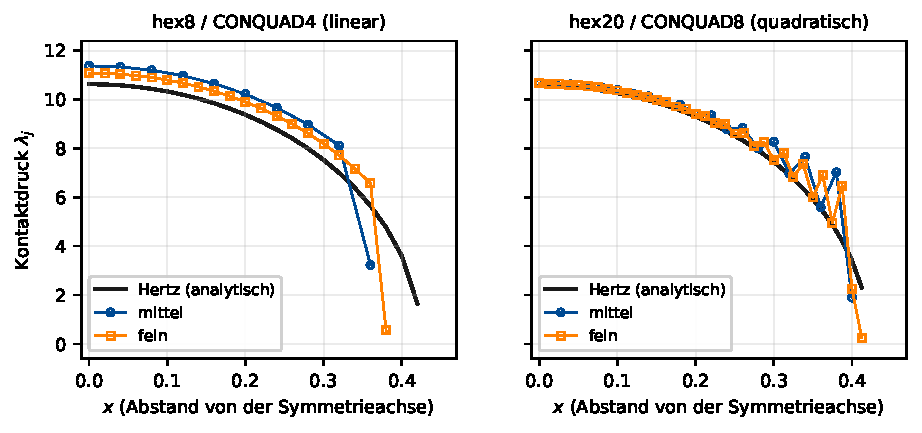
\includegraphics[width=\linewidth]{hertz_druckprofil.pdf}
\caption[Hertz-Kontakt: berechnetes Druckprofil gegen die analytische Lösung]{Kontaktdruck
$\lambda_j$ an den Slave-Knoten gegen die Hertz'sche Halbellipse \eqref{eq:hertz}, je Elementtyp
für zwei Netzfeinheiten. \emph{Links:} lineare Elemente liefern ein \emph{glattes} Profil, dessen
Maximum aber systematisch zu hoch liegt und mit Verfeinerung sinkt. \emph{Rechts:} quadratische
Elemente treffen das Maximum auf $\sim\!1\,\%$, zeigen dafür die Knoten-zu-Knoten-Oszillation
quadratischer Mortar-Kontaktdrücke, am stärksten am Rand der Kontaktzone. Die eingezeichnete
Hertz-Kurve gehört jeweils zur feinen Variante; $p_0$ hängt über $P'$ schwach vom Netz ab.
Erzeugt aus \file{Control\_Tests/08\_hertz/hertz\_profile\_*.csv}.}
\label{fig:hertz}
\end{figure}

\begin{center}
\small
\begin{tabular}{lccccc}
\toprule
Netz & $a_{\text{num}}$ / $a_{\text{Hertz}}$ & Fehler $a$ & $p_{0,\text{num}}$ / $p_{0,\text{Hertz}}$ & Fehler $p_0$ & Zickzack \\
\midrule
hex8, mittel  & $0{,}4094$ / $0{,}4270$ & $4{,}1\,\%$ & $11{,}379$ / $10{,}674$ & $6{,}6\,\%$ & $5{,}3\,\%$ \\
hex8, fein    & $0{,}4243$ / $0{,}4252$ & $0{,}2\,\%$ & $11{,}082$ / $10{,}629$ & $4{,}3\,\%$ & $3{,}0\,\%$ \\
hex20, mittel & $0{,}4434$ / $0{,}4227$ & $4{,}9\,\%$ & $10{,}675$ / $10{,}568$ & $1{,}0\,\%$ & $10{,}1\,\%$ \\
hex20, fein   & $0{,}4358$ / $0{,}4227$ & $3{,}1\,\%$ & $10{,}673$ / $10{,}567$ & $1{,}0\,\%$ & $7{,}8\,\%$ \\
\bottomrule
\end{tabular}
\end{center}

\noindent Die beiden Elementordnungen irren in \emph{verschiedene} Richtungen, und das ist der
eigentliche Befund dieses Tests:

\begin{itemize}\itemsep2pt
  \item \textbf{Linear (\code{hex8}/CONQUAD4).} Das Profil ist glatt, der Maximaldruck aber um
        $4$--$7\,\%$ zu hoch. Ursache ist die Geometrie: lineare Facetten bilden die gekrümmte
        Oberfläche als Polygonzug ab, die Kontaktzone wird zu schmal, und bei gleicher Gesamtkraft
        muss der Druck darin entsprechend zu hoch ausfallen. Der Fehler sinkt mit Verfeinerung
        ($6{,}6\to4{,}3\,\%$), also erwartungsgemäß.
  \item \textbf{Quadratisch (\code{hex20}/CONQUAD8).} Der Maximaldruck stimmt auf $1{,}0\,\%$ --
        die gekrümmte Facette wird über die Formfunktionsauswertung an den Gauß-Punkten
        tatsächlich erfasst (Abschnitt~\ref{sec:subcells}). Dafür oszilliert der Druck von Knoten
        zu Knoten um $8$--$10\,\%$. Das ist der Ecke/Mittelknoten-Effekt quadratischer
        Mortar-Kontaktdrücke: Eck- und Mittelknoten tragen unterschiedlich gewichtete
        Multiplikatoren (Abschnitt~\ref{sec:basistrafo}, die Gewichte $\tfrac{7}{18}$ und
        $\tfrac29$). Im Inneren der Kontaktzone dämpft die duale Basis ihn, am Rand bleibt er, und
        er sinkt nur langsam mit Verfeinerung ($10{,}1\to7{,}8\,\%$).
\end{itemize}

\noindent Dass die Oszillation kein \emph{Auswertungs}artefakt ist, wird eigens geprüft: der
Report berechnet sie zweimal, einmal aus $\lambda_j$ direkt und einmal aus der über den ganzen
Knotenträger verteilten Knotenkraft $p_{F,j}$ \eqref{eq:pforce}. Am Rand der Kontaktzone könnten
beide Lesarten auseinanderlaufen, weil $\lambda_j$ dort mit $\tilde D_{jj}^{-1}$ skaliert
(Abschnitt~\ref{sec:lambdadeutung}). Sie tun es nicht -- die Zickzack-Werte stimmen in beiden
Lesarten auf drei Stellen überein (Spalten \code{zickzk\%} und \code{zz\_F\%} des Reports). Die
Oszillation ist damit als Diskretisierungseigenschaft nachgewiesen und nicht als Artefakt der
Auswertung. Die \emph{übertragene Gesamtkraft} ist bei beiden Elementordnungen korrekt; abweichend
ist ausschließlich die punktweise Verteilung.

\medskip
\noindent \textbf{Bewertung.} Der Hertz-Test bestätigt die Formulierung, aber er ist -- anders als
die Zwei-Block-Reihe -- \emph{kein} Genauigkeitsnachweis in Maschinengenauigkeit, und er kann es
nicht sein: Hertz ist eine Halbraum-Näherung, das Modell ist endlich und uniform vernetzt (rund
$11$ bis $22$ Elemente über die halbe Kontaktbreite), und die Kontaktzone endet zwischen zwei
Knoten, sodass ihre Halbbreite $a$ nur bis auf einen Knotenabstand bestimmt ist -- die
$3$--$5\,\%$ in der Spalte ``Fehler $a$'' sind im Wesentlichen genau das. Was der Test zeigt, ist
zweierlei: erstens, dass die Größenordnungen und die Form stimmen und sich mit Verfeinerung in die
richtige Richtung bewegen; zweitens, dass die verbleibenden Abweichungen \emph{benannte}
Diskretisierungseffekte sind -- Facettengeometrie bei linearen, Ecke/Mittelknoten bei
quadratischen Elementen -- und keine Anzeichen eines Fehlers in der Formulierung. Ein Restpunkt
bleibt offen: die Knoten-zu-Knoten-Oszillation quadratischer Kontaktdrücke am Kontaktrand ist mit
$\sim\!10\,\%$ nicht klein und konvergiert langsam. Sie ist ein Genauigkeits-, kein
Konvergenzproblem -- alle vier Hertz-Varianten konvergieren -- und betrifft die punktweise
Druckauswertung, nicht die übertragene Kraft.

% =====================================================================
\section{Testbeispiel: Ausziehversuch nach Dejori}
\label{sec:testbeispiel}

Als anwendungsnahes Testbeispiel wird der Ausziehversuch eines Kopfbolzendübels aus einem
Betonquader nachgerechnet (Versuchsreihe VA1, Einbindetiefe 6\,cm). Er ist das eigentliche
Zielproblem des Mortar-Kontakts in diesem Projekt: der Anker ist ein eigener Körper, der nur über
den Kontakt Kräfte in den Beton einleitet, und die Netze beider Körper sind an der Kontaktfläche
nichtkonform. Anders als die Patch- und Referenztests aus Abschnitt~\ref{sec:verif} ist dieses
Beispiel weder analytisch lösbar noch spannungshomogen -- es zeigt, wie sich die Formulierung
unter realen Bedingungen verhält, einschließlich ihrer Grenzen.

\subsection{Modell}
Der Beton ist mit gradientenerweiterter Schädigungsplastizität (\code{GCDP}) modelliert, Anker und
Auflager linear-elastisch ($E=210\,000$\,MPa). Das Modell ist ein 4\,mm dicker Scheibenschnitt; die
ausgewertete Kraft wird mit dem Faktor 20 auf die reale Probenbreite von 80\,mm hochgerechnet. Der
Anker wird verschiebungsgesteuert um bis zu 1{,}1\,mm nach oben gezogen. Der Kontakt zwischen Stahl
und Beton ist in \textbf{sechs} getrennte Mortar-Constraints zerlegt (links und rechts, je
Schaftflanke, Kopfunterseite und Kopfflanke); der Beton ist jeweils die Slave-Seite. Die Zerlegung
ist bewusst so gewählt: an der 90$^\circ$-Kante zwischen Schaft und Kopf wäre eine gemeinsame
Kontaktfläche mit mehrdeutiger, gemittelter Knotennormale behaftet
(Abschnitt~\ref{sec:normalen}); getrennte Constraints erhalten dort die flächeneigene Normale.

Gerechnet wird dasselbe Modell zweimal: einmal linear (\code{GC3D8} für den Beton, Kontaktelemente
\code{CONQUAD4}) und einmal quadratisch (\code{GC3D20R}, \code{CONQUAD8}). Die beiden Netze sind
\emph{geometrisch identisch} -- gleiche Elementzahl (9162 Betonelemente), gleiche sechs
Kontaktflächen mit gleicher Facettenzahl, und die Eckknoten stimmen auf Maschinengenauigkeit
überein; das quadratische Netz hat lediglich zusätzliche Kantenmittelknoten.

Die Auflager sind als elastische Bettung über \code{directionalspringpenalty} abgebildet. Da dieser
Constraint eine unabhängige Einzelfeder der Steifigkeit \code{penalty} auf jeden Knoten des
Knotensets setzt, ist die Gesamtsteifigkeit einer Auflagerfläche knotenzahl- und damit
elementordnungsabhängig. Beide Rechnungen verwenden dieselbe Gesamtbettung von $9200$\,N/mm je
Auflager, umgerechnet über die Knotenzahl: \code{penalty}${}=920$ bei $10$ Knoten (hex8) und
\code{penalty}${}=400$ bei $23$ Knoten (hex20).

\subsection{Ergebnis}
Abbildung~\ref{fig:pot} stellt beide Rechnungen den drei Laborversuchen gegenüber.

\begin{figure}[htbp]
\centering
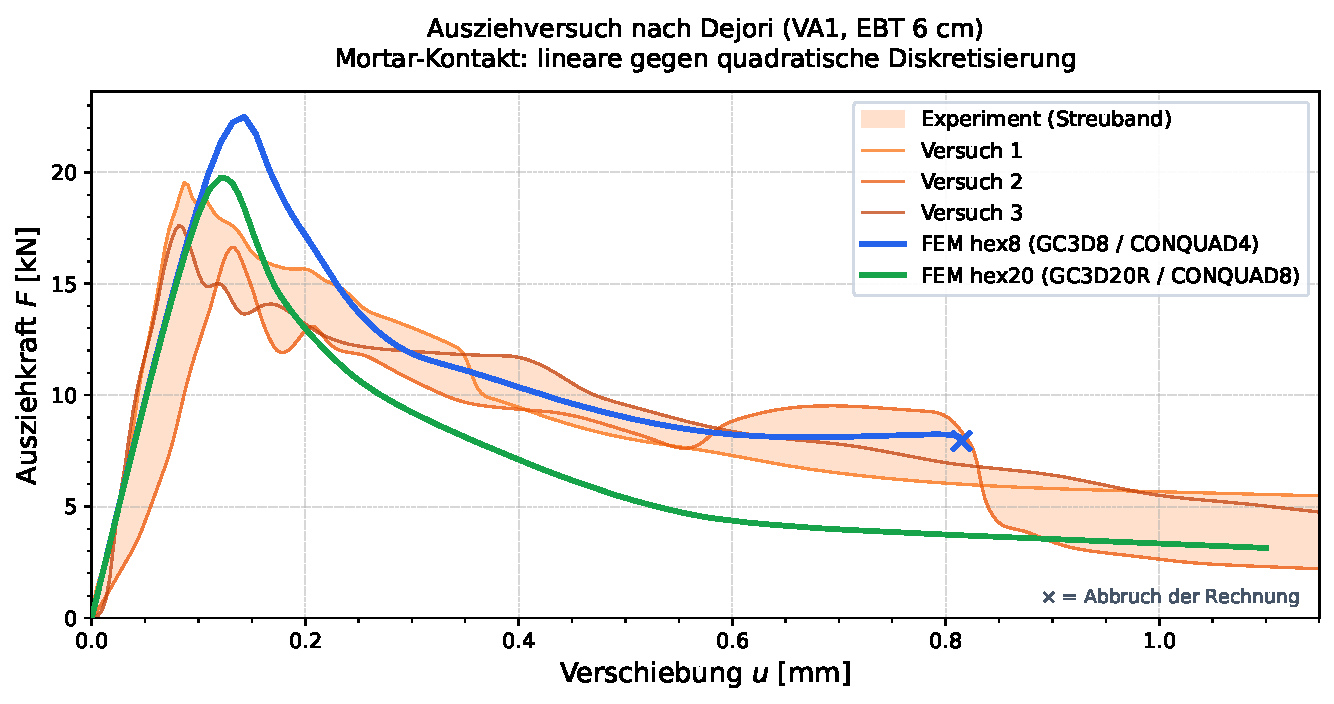
\includegraphics[width=0.95\linewidth]{force_disp_hex8_vs_hex20.pdf}
\caption[Ausziehversuch nach Dejori: Kraft-Weg-Kurven]{Ausziehversuch nach Dejori:
Kraft-Weg-Kurven der linearen (hex8) und der quadratischen
(hex20) Diskretisierung gegen das Streuband der drei Laborversuche. Beide Rechnungen verwenden
dieselbe Gesamt-Auflagerbettung. Das Kreuz markiert jeweils das
Ende der Rechnung. Erzeugt mit \file{POT\_Dejori/plot\_comparison.py}.}
\label{fig:pot}
\end{figure}

\begin{center}
\small
\begin{tabular}{lccc}
\toprule
 & Sekantensteifigkeit ($u\le0{,}03$\,mm) & $F_{\max}$ & $u$ bei $F_{\max}$ \\
\midrule
hex8 (\code{GC3D8}/\code{CONQUAD4})    & $199{,}1$\,kN/mm & $22{,}50$\,kN & $0{,}143$\,mm \\
hex20 (\code{GC3D20R}/\code{CONQUAD8}) & $197{,}7$\,kN/mm & $19{,}85$\,kN & $0{,}121$\,mm \\
\midrule
Versuch 1 & --- & $19{,}53$\,kN & $0{,}087$\,mm \\
Versuch 2 & --- & $16{,}63$\,kN & $0{,}133$\,mm \\
Versuch 3 & --- & $17{,}63$\,kN & $0{,}082$\,mm \\
\bottomrule
\end{tabular}
\end{center}

\paragraph{Anfangssteifigkeit: elementordnungsunabhängig.}
Die Sekantensteifigkeiten stimmen auf $0{,}7\,\%$ überein. Das ist das erwartete Ergebnis: im
nahezu elastischen Bereich, vor Einsetzen nennenswerter Schädigung, darf die Elementordnung die
Systemsteifigkeit kaum beeinflussen, und der Mortar-Kontakt überträgt in beiden Fällen dieselbe
Last. Es bestätigt zugleich die Referenztests aus \file{Control\_Tests}, in denen hex8, hex20 und
hex20R exakt dieselbe Steifigkeit liefern. Für den verbleibenden Unterschied gilt: das
quadratische, reduziert integrierte Modell ist geringfügig \emph{weicher} -- die theoretisch
richtige Richtung, da der trilineare Ansatzraum im 20-Knoten-Serendipity-Raum enthalten ist und
reduzierte Integration die Steifigkeit zusätzlich senkt.

\paragraph{Traglast: Einfluss der Diskretisierung.}
Am Peak trennen sich die Kurven. Die quadratische Rechnung trifft mit $19{,}85$\,kN die Oberkante
des Versuchsstreubands ($16{,}6\ldots19{,}5$\,kN), die lineare überschätzt mit $22{,}50$\,kN alle
drei Versuche um $15$ bis $35\,\%$ und erreicht den Peak zudem später ($0{,}143$ statt
$0{,}121$\,mm). Das ist ein echter Diskretisierungseffekt: der Ausziehversuch ist am Bolzenkopf
lokalisierungsdominiert, und lineare Elemente verschmieren den dortigen Dehnungsgradienten über die
Elementlänge. Die lokale Spannungsspitze wird dadurch unterschätzt, die Schädigung setzt verspätet
ein, und die Kurve läuft auf einen höheren, späteren Peak. Im entfestigenden Ast liegt die lineare
Rechnung durchgehend über der quadratischen und näher am Versuchsband -- bei einem
lokalisierenden Material ist das kein Qualitätsmerkmal, sondern Ausdruck der gröberen Auflösung der
Schädigungszone.

\subsection{Abbruchverhalten und Rechenaufwand}
Die beiden Rechnungen enden aus \emph{unterschiedlichen} Gründen; das ist für die Bewertung der
Kurven wesentlich.

\paragraph{hex8: Materialversagen.}
Die lineare Rechnung läuft bis $u=0{,}795$\,mm, also weit über den Peak hinaus, und bricht dort im
entfestigenden Ast ab: die Kurve endet mit \emph{senkrechter Tangente}
($\mathrm dF/\mathrm du\to-\infty$; über die letzten Inkremente $-452$\,kN/mm, während $u$ praktisch
stehenbleibt). Der Beton kann der aufgezwungenen Verschiebung nicht mehr folgen -- das Material
versagt. Der Löser meldet entsprechend, dass die Schrittweite nicht weiter reduziert werden kann.
Die Kurve ist damit inhaltlich vollständig: Anstieg, Traglast und ein großer Teil des
Nachbruchbereichs sind erfasst. Aufwand: $184$ Inkremente, $13$ Cutbacks, rund $1200$
Newton-Iterationen, etwa $25$ Minuten Rechenzeit.

\paragraph{hex20: händischer Abbruch.}
Die quadratische Rechnung versagt nicht, sie kommt nicht mehr voran. Nach $5902$ Inkrementen,
$302$ Cutbacks und rund $34\,000$ Newton-Iterationen war sie erst bei $u=0{,}838$\,mm, also
$76\,\%$ der vorgegebenen $1{,}1$\,mm -- bei einer Laufzeit von $49{,}5$ Stunden
(gut zwei Tagen). Die Schrittweite war zu diesem Zeitpunkt auf etwa $10^{-4}$\,mm je Inkrement
gefallen, bei nahezu waagrechter Kurve ($\mathrm dF/\mathrm du\approx-2$\,kN/mm). Hochgerechnet
hätte allein der verbleibende Weg nochmals mehr als einen Tag benötigt, ohne dass ein qualitativ
neues Ergebnis zu erwarten gewesen wäre. Die Rechnung wurde deshalb händisch abgebrochen; das
Kreuz in Abbildung~\ref{fig:pot} markiert diesen Punkt, nicht ein Versagen.

\paragraph{Einordnung.}
Der Aufwandsunterschied -- rund $29$-mal so viele Newton-Iterationen bei $3{,}5$-mal so vielen
Knoten -- ist nicht allein Netzgröße. Er ist auch die praktische Auswirkung der fehlenden
konsistenten Linearisierung (Abschnitt~\ref{sec:frozen}): ohne die geometrischen Ableitungen ist
der Konvergenzradius kleiner, das Verfahren greift häufiger zu Cutbacks, und die Schrittweite
erholt sich im entfestigenden Bereich nicht mehr. Genau hier läge der Gewinn einer konsistenten
Linearisierung (Abschnitt~\ref{sec:ausblick:lin}) -- nicht in der Genauigkeit der Kurve, sondern darin,
sie überhaupt in vertretbarer Zeit zu Ende rechnen zu können.

% =====================================================================
\section{Zusammenfassung}
\label{sec:zusammenfassung}

Der auf Branch \code{0\_mortarcontact} implementierte reibungsfreie Mortar-Kontakt überträgt Kräfte
zwischen nichtkonformen Netzen über eine schwach (im integralen Mittel) durchgesetzte
Nichtdurchdringungsbedingung. Die tragenden Bausteine sind:
\begin{itemize}\itemsep2pt
  \item eine \textbf{segmentbasierte Integration} mit BVH-Nachbarsuche, Hilfsebenen-Projektion,
        Sutherland--Hodgman-Clipping und Grad-5-Quadratur (7-Punkt-Dreiecksregel nach \citealt{dunavant1985}),
        wobei der erhöhte Grad die nichtlineare Projektion auffängt (\citealp{farah2015});
  \item \textbf{duale Lagrange-Multiplikatoren} (\citealp{wohlmuth2000}), die $\bm D$ diagonalisieren und die
        Koppelmatrizen $\bm D,\bm M$ samt gewichtetem Spalt $\tilde g_j$ liefern, mit garantierter
        Zeilensummen-Identität (Impulserhaltung);
  \item eine \textbf{Basistransformation} für quadratische Elemente (\citealp{popp2012}; im Code der
        Farah-Wert $\alpha=\tfrac13$) zur Sicherung positiver dualer Gewichte, plus lineare
        \textbf{Sub-Cells} fürs Clipping (\citealp{puso2008});
  \item die \textbf{semiglatte NCP-Formulierung} der Signorini-Bedingung (\citealp[Gl.~(55)]{gitterle})
        gelöst per \textbf{PDASS}/semismooth Newton (\citealp{hueber2005}).
\end{itemize}
Die Formulierung besteht die Kontakt-Patch-Tests in 2D und 3D (linear und quadratisch, konform und
nichtkonform) bei geraden Facettenkanten in Maschinengenauigkeit; bei gekrümmten Kanten gilt der
Patch-Test im dokumentierten Näherungsrahmen (Abschnitt~\ref{sec:verif}). Coulomb-Reibung und
statische Kondensation sind nicht umgesetzt; ihre Bausteine und die dafür erforderlichen
Erweiterungen sind in den Abschnitten~\ref{sec:ausblick:reibung}
und~\ref{sec:ausblick:kondensation} benannt.

\medskip
\noindent Die bewusst in Kauf genommenen Einschränkungen sind an ihren jeweiligen Stellen benannt:
die fehlende geometrische Linearisierung und der Staffelungsfehler der eingefrorenen Geometrie
(Abschnitt~\ref{sec:frozen}), die nur näherungsweise Integration über gekrümmte Facetten
(Abschnitt~\ref{sec:subcells}), die möglichen negativen Knotengewichte des CONQUAD9 bei
Teilüberdeckung (Abschnitt~\ref{sec:basistrafo}) sowie die impliziten Annahmen und Rückfallpfade
der Implementierung (Abschnitt~\ref{sec:implnotes}).

% =====================================================================
\section{Ausblick}
\label{sec:ausblick}

\subsection{Konsistente Linearisierung}
\label{sec:ausblick:lin}

Der nächste substanzielle Entwicklungsschritt ist die \emph{konsistente Linearisierung} des
Kontaktbeitrags. Wie in Abschnitt~\ref{sec:frozen} gezeigt, ist die assemblierte Tangente exakt
für das Residuum bei eingefrorener Geometrie, enthält aber die Ableitungen der Geometrie selbst
nicht -- $\partial\bm D/\partial\bm x$, $\partial\bm M/\partial\bm x$ und
$\partial\bm n_j/\partial\bm x$ --, und diese Terme sind mit $0{,}27\ldots2{,}0$ von
$\max|\bm K|$ nicht klein.

Sie zu ergänzen ist kein Zusatzterm, sondern erfordert Ableitungen entlang der \emph{gesamten}
Segmentierungskette. Der Reihe nach sind das:
\begin{enumerate}\itemsep2pt
  \item die Knotennormale $\bm n_j$ nach \eqref{eq:facetnormal} -- die Ableitung einer normierten
        Summe von Kreuzprodukten;
  \item die Hilfsebene: Stützpunkt $\bm p_0$, Normale und Tangentenbasis $\bm t_1,\bm t_2$, die
        alle von den Koordinaten der Slave-Sub-Zelle abhängen;
  \item die Projektion beider Facetten in diese Ebene;
  \item die Eckpunkte des geclippten Polygons: durchgereichte Ecken hängen unmittelbar von den
        Facettenkoordinaten ab, Schnittpunkte über die Geradenschnittformel von je vier
        Eckpositionen;
  \item die Zell-Jacobi-Determinante der Integrationsdreiecke und die Lage der Gauß-Punkte;
  \item die Newton-Rückabbildung $\bm\xi(\bm x_{\text{gp}})$ in beide Naturkoordinaten, deren
        Ableitung über den Satz über implizite Funktionen aus der Element-Jacobi-Matrix folgt;
  \item die \emph{dualen} Formfunktionen selbst: $\bm A_e$ wird aus der Segmentquadratur gebildet
        (Abschnitt~\ref{sec:dual}) und hängt damit ebenfalls von den Koordinaten ab;
  \item daraus schließlich $\partial N/\partial\bm x$, $\partial\Phi/\partial\bm x$ und damit
        $\partial\bm D/\partial\bm x$ und $\partial\bm M/\partial\bm x$.
\end{enumerate}
Diese Gliederung ist keine eigene: \citet[Anh.~A]{popp2010} führen für dieselbe Formulierung
genau sechs zu linearisierende Größen auf -- Normalen- und Tangentenvektoren, die Integrale der
Mortar-Matrizen, die gewichteten Spalte, die Gauß-Punkt-Koordinaten, die Eckpunkte der
Integrationszellen und die dualen Formfunktionen -- und geben die zugehörigen Richtungsableitungen
in den Abschnitten A.1 bis A.6 an. \citet[Kap.~4]{farah} führt dieselbe Kette aus. Zum Aufwand
äußern sich \citet[Anh.~A]{popp2010} unmissverständlich: ``the computation of directional
derivatives accounts for a significant portion of the implementation effort associated with our
method''.

\paragraph{Zwei Eigenschaften, die dabei zu bedenken sind.}
Erstens ist Schritt~4 nur \emph{stückweise} glatt: wandert ein Eckpunkt über eine Clip-Kante, so
ändert sich die Anzahl der Polygonecken, und die Ableitung springt. Auch eine vollständige
Linearisierung ist an diesen Übergängen unstetig.

Zweitens ist die \emph{Symmetrie} keine Selbstverständlichkeit. \citet{hiermeier2018} halten fest,
dass die meisten Mortar-Formulierungen für reibungsfreien Kontakt in ihrer konsistent
linearisierten Form auf eine unsymmetrische Jacobi-Matrix führen, obwohl sie von einem skalaren
Potential ausgehen:
\begin{quote}
\small ``it is not immediately obvious why most mortar-type contact formulations for frictionless
contact lead to a non-symmetric Jacobian matrix in their consistently linearized form \ldots\ Only
a deeper insight reveals the neglected terms and certain assumptions in the published
formulations.'' \hfill \citep[S.~3 des Manuskripts]{hiermeier2018}
\end{quote}
Sie zeigen zugleich, dass dies \emph{kein} notwendiger Preis der Konsistenz ist: eine strenge
Variation des zugrunde liegenden Potentials führt sehr wohl auf ein symmetrisches System,
allerdings um den Preis erheblich teurerer Terme zweiter Ordnung. Sie entwickeln daher beide
Varianten nebeneinander -- die strenge, symmetrische und eine vereinfachte, unsymmetrische, die
die Impulserhaltung dennoch wahrt. Für eine Umsetzung hier heißt das: die heute symmetrische
Sattelpunktstruktur (Abschnitt~\ref{sec:loesung}) bliebe nur auf dem strengen Weg erhalten, und
die Wahl zwischen beiden schlägt auf Löser und Vorkonditionierer durch.

Günstig ist dagegen die Schnittstellenseite: die Linearisierungsterme sind \emph{additive}
Beiträge zu $\bm K$ und damit genau das, was ein Constraint beisteuern kann. Anders als die
statische Kondensation (Abschnitt~\ref{sec:ausblick:kondensation}) erfordert die Linearisierung
\textbf{keine} Erweiterung des Rahmenwerks.

\paragraph{Ein möglicher Weg in vier Stufen.}
Der Übergang muss nicht in einem Schritt erfolgen. Jede der folgenden Stufen ist für sich lauffähig
und -- das ist der eigentliche Punkt -- für sich \emph{messbar}: Test~09 beziffert die verbleibende
Lücke zwischen $\bm K$ und dem Differenzenquotienten bei voller Geometrie, Test~12 den
Staffelungsfehler. Nach jeder Stufe steht damit fest, wie viel sie gebracht hat.

\begin{enumerate}\itemsep3pt
  \item[\textbf{(I)}] \textbf{Geometrie nachführen, ohne zu linearisieren.} $\bm n_j,\bm D,\bm M$
        werden in jeder Newton-Iteration neu ausgewertet statt einmal je Increment. Der
        Staffelungsfehler (Abschnitt~\ref{sec:staffelordnung}) entfällt damit vollständig, die
        konvergierte Lösung ist geometrisch exakt. Der Preis: $\bm K$ ist dann nicht einmal mehr
        die Jacobi-Matrix des eingefrorenen Residuums, die Konvergenz also möglicherweise
        schlechter. Ob es netto hilft, ist eine reine Messfrage -- und diese Stufe ist zugleich
        diejenige, die den geringsten Eingriff erfordert. \emph{Zur Einordnung:} MOOSE erzeugt das
        Mortar-Segment-Netz bei verschobenem Netz je Residuumsauswertung neu, \code{Abaqus/Standard}
        stellt den Kontaktzustand dagegen je Increment fest und behandelt Statuswechsel als
        \emph{severe discontinuity iteration}. Beide Vorgehensweisen sind in Gebrauch; Stufe~(I)
        wechselt von der zweiten zur ersten.
  \item[\textbf{(II)}] \textbf{$\partial\bm n_j/\partial\bm x$.} Der in sich geschlossenste Term
        und der einzige, der ohne die Segmentierungskette auskommt. Er lässt sich isoliert
        prüfen, indem man $\bm D$ und $\bm M$ im Differenzenquotienten festhält und nur die
        Normalen mitführt.
  \item[\textbf{(III)}] \textbf{$\partial\bm D/\partial\bm x$ und $\partial\bm M/\partial\bm x$
        über die Rückabbildung} (Schritte 6 und 7 oben), bei zunächst als fest behandelter
        Clip-Geometrie. Damit ist der überwiegende Teil der Formfunktionsabhängigkeit erfasst.
  \item[\textbf{(IV)}] \textbf{Die Segmentierungsgeometrie} (Schritte 2 bis 5): Hilfsebene,
        Projektion, Clip-Eckpunkte, Zell-Jacobi. Der aufwendigste und heikelste Teil, und der
        einzige, der die stückweise Glattheit aus dem vorigen Absatz berührt.
\end{enumerate}

\noindent Als Abnahmekriterium eignet sich unmittelbar Test~09: Teil~2 dieses Tests differenziert
das Residuum mit bei jeder Störung \emph{neu berechneter} Geometrie und weist die Abweichung
gegenüber $\bm K$ aus. Sie beträgt heute $0{,}27\ldots2{,}0$ und müsste nach Stufe~(IV) auf das
Niveau von Teil~1 fallen, also auf etwa $10^{-8}$. Solange sie das nicht tut, fehlt ein Term --
ein Kriterium, das kein Ermessen zulässt.

\paragraph{Abgrenzung: was die Linearisierung nicht leistet.}
Sie verbessert weder die Genauigkeit über das Verschwinden des Staffelungsfehlers hinaus (der
liegt bereits bei $10^{-4}\ldots10^{-3}$ und wird über die Schrittweite kontrolliert) noch die in
Abschnitt~\ref{sec:scalelimit} beschriebene Skalengrenze des Multiplikator-Residuums noch das
Verhalten des CONQUAD9 bei Teilüberdeckung. Und sie ist nicht das einzige Mittel gegen kleine
Konvergenzradien: Produktionscodes fangen genäherte Tangenten mit einer
\emph{Globalisierung} auf -- Line-Search oder gedämpftes Newton-Verfahren
(\citealp{deuflhard2004}; \citealp{deluca1996}) --, die hier ebenfalls nicht umgesetzt ist und
ungleich weniger Aufwand erfordert. Welcher der beiden Hebel im konkreten Fall der wirksamere
ist, lässt sich vorab nicht entscheiden; Stufe~(I) liefert die Zahlen, an denen es sich
beurteilen lässt.

\subsection{Selbstkontakt}
\label{sec:ausblick:selbst}

Die Formulierung ist auf ein festes, disjunktes Flächenpaar aufgebaut und deckt damit den
Selbstkontakt -- die Berührung einer Oberfläche mit sich selbst unter großer Verformung -- nicht ab.
Die Paarung von Slave- und Masterfläche erfolgt einmalig bei der Instanziierung, womit auch die
Zahl der Multiplikatoren feststeht; die Vorzeichenkonvention des Spalts setzt zwei getrennte Körper
voraus; eine Ausschlussregel für die eigene und die angrenzenden Facetten einer Slave-Facette
existiert nicht, und für einen Knoten, der beiden Flächen angehörte, wäre die flächengewichtete
Knotennormale nach \eqref{eq:facetnormal} nicht eindeutig definiert.

Die bindende Einschränkung ist dabei algebraischer Natur. Für deckungsgleiche Facetten gilt
$\bm M=\bm D$ exakt, sodass der gewichtete Spalt
\begin{equation*}
\tilde g_j = -\sum_k D_{jk}\,(\bm x_k\!\cdot\!\bm n_j) + \sum_l M_{jl}\,(\bm x_l\!\cdot\!\bm n_j)
\end{equation*}
für jede Konfiguration identisch verschwindet. Die zugehörige $\lambda$-Zeile von $\bm K$ hebt sich
auf, sobald ein solcher Knoten aktiv wird, und das Gesamtsystem ist singulär. Der Konstruktor prüft
daher auf gemeinsame Knoten beider Flächen und weist solche Konfigurationen zurück
(Abschnitt~\ref{sec:implnotes}; Regressionstest in \file{07\_patch\_test\_2d}).

Von den Bausteinen, die eine Selbstkontaktbehandlung erfordert, ist einer bereits vorhanden: die
binäre Bounding-Volume-Hierarchie über die Kontaktfläche (\code{build\_bvh},
Abschnitt~\ref{sec:geometrie}) entspricht der Suchstruktur, die \citet{yang2008} für denselben
Zweck verwenden. Sie ist für sich genommen jedoch nicht hinreichend
\citep[S.~764]{yang2008}:

\begin{quote}
\small ``[\ldots] it might be as inefficient as $\mathcal{O}(n^2)$ for a contact surface with $n$
elements since the bounding volumes of adjacent subsurfaces always intersect with each other.''
\end{quote}

\noindent Die Hüllkörper benachbarter Facetten schneiden sich stets, sodass eine reine
Näherungssuche gerade jene Paare zurückliefert, die auszuschließen sind. \citet{yang2008} ergänzen
sie um ein Krümmungskriterium als hinreichende Bedingung für die Abwesenheit von Selbstkontakt,
das sie \citet{volino2000} entnehmen \citep[S.~764]{yang2008}. Im Original lautet es
\citep[Abschn.~3.2.2, S.~134]{volino2000} (dort als Aufzählung gesetzt):

\begin{quote}
\small ``Let $S$ be a continuous surface in Euclidean space, delimited by one contour $C$. If
there exists a vector $V$ for which $N\cdot V>0$ at (almost) every point of $S$ ($N$ being the
normal vector of the surface at the considered point), and the projection of $C$ on a plane
orthogonal to $V$ along the direction of $V$ has no self-intersections, then there are no
self-collisions on the surface $S$.''
\end{quote}

\noindent \citet{yang2008} geben es sinngemäß wieder; die Einschränkung ``at (almost) every
point'' entfällt dort.

\noindent In Verbindung mit einem $\mathcal{O}(1)$-Adjazenztest lassen sich damit benachbarte
Teilflächen ausschließen, ohne sie geometrisch zu schneiden. Hinzu kommt ein Facet-Sorting, das die
Mortar-Integrale auf zusammenhängenden Element-Patches definiert hält. Beide Bestandteile sind
nicht implementiert; ihre Ergänzung wäre ein eigenständiger Entwicklungsschritt.

\subsection{Coulomb-Reibung}
\label{sec:ausblick:reibung}

Die Formulierung überträgt ausschließlich Normalkräfte. Die Erweiterung auf Coulomb-Reibung ist in
der Mortar-Literatur vollständig ausgearbeitet und fügt sich in dieselbe semiglatte Struktur ein;
ihre Bausteine lassen sich daher genau benennen.

Kontinuierlich treten zu den Normalbedingungen \eqref{eq:kkt} die Reibbedingungen
\begin{equation}
\Psi := \|\bm t_\tau\| - \mathcal F\,p_n \le 0,
\qquad
\bm v_{\tau,\text{rel}} + \beta\,\bm t_\tau = \bm 0,
\qquad
\beta \ge 0,
\qquad
\beta\,\Psi = 0
\label{eq:coulomb}
\end{equation}
-- ohne Betragsstriche, weil $p_n\ge0$ die Achse des Coulomb-Kegels ist
(Abschnitt~\ref{sec:vorzeichenkonvention}) -- mit dem Reibbeiwert $\mathcal F$ und der relativen Tangentialgeschwindigkeit
$\bm v_{\tau,\text{rel}}$ \citep[Gl.~(10)--(13), S.~546--547]{gitterle}. Sie zerfallen in zwei
Zustände: \emph{Haften} ($\Psi<0$, erzwingt $\bm v_{\tau,\text{rel}}=\bm 0$) und \emph{Gleiten}
($\Psi=0$, die Tangentialspannung stellt sich der Relativbewegung entgegen).

Diskret werden auch diese Bedingungen in \emph{eine} nichtglatte Funktion gefasst -- genau wie die
Normalbedingung in \eqref{eq:ncp}. Ausgangspunkt ist die Tresca-Form mit konstanter Reibschranke
$b_j$ \citep[Gl.~(58)]{gitterle}; ersetzt man $b_j$ durch die lastabhängige Coulomb-Schranke
$b_j=\mathcal F\max(0,\lambda_j-c_n\tilde g_j)$ \citep[Gl.~(60)]{gitterle} und löst die
geschachtelten Maxima auf, so ergibt sich
\begin{equation}
C_{\tau,j} = \max\!\big(\mathcal F(\lambda_j-c_n\tilde g_{j}),\;
\|\bm\lambda_{\tau,j}+c_t\,\tilde{\bm u}_{\tau,\text{rel},j}\|\big)\,\bm\lambda_{\tau,j}
- \mathcal F\max\!\big(0,\lambda_j-c_n\tilde g_{j}\big)
\big(\bm\lambda_{\tau,j}+c_t\,\tilde{\bm u}_{\tau,\text{rel},j}\big) = \bm 0
\label{eq:ncptau}
\end{equation}
mit $c_n,c_t>0$ (\citealp[Gl.~(61)/(62)]{gitterle}; in der hier notierten allgemeinen Form
\citealp[Gl.~(3.60)/(3.61)]{farah}). Wie $c_n$ beeinflussen beide Parameter allein das
Konvergenzverhalten, nicht die Lösung.

Für die vorliegende Implementierung folgen daraus vier konkrete Änderungen:

\begin{itemize}\itemsep2pt
  \item \textbf{Multiplikator wird vektoriell.} Statt eines skalaren Normalmultiplikators je
        Slave-Knoten (Abschnitt~\ref{sec:koppelmatrizen}) sind $\dim$ Freiheitsgrade zu
        instanziieren; die Kontaktkraft ist dann nicht mehr auf $\bm n_j$ beschränkt. Die
        Koppelmatrizen $\bm D,\bm M$ selbst bleiben unverändert -- sie sind bereits als
        $D_{jk}\bm I$ definiert \eqref{eq:DM}.
  \item \textbf{Eine neue kinematische Größe.} Der gewichtete relative Schlupfzuwachs
        $\tilde{\bm u}_{\tau,\text{rel},j}$ tritt neben den gewichteten Spalt. Er ist
        \emph{pfadabhängig} und muss über die Increments akkumuliert werden, und er ist als
        Ratengröße nur dann brauchbar, wenn seine Auswertung bezugsystemunabhängig erfolgt
        -- ein Punkt, den \citet{gitterle} eigens behandeln. Der Spalt allein ist
        konfigurationsabhängig, der Schlupf dagegen geschichtsbehaftet; die eingefrorene
        Geometrie (Abschnitt~\ref{sec:frozen}) berührt damit hier mehr als beim Normalkontakt.
  \item \textbf{Dreiwertiges Active Set.} An die Stelle der Aufteilung aktiv/inaktiv tritt
        inaktiv/haftend/gleitend. Da die Reibschranke in \eqref{eq:ncptau} den Normaldruck
        enthält, sind Normal- und Tangentialzweig gekoppelt und nicht getrennt lösbar.
  \item \textbf{Zweiter algorithmischer Parameter.} $c_t$ balanciert $\bm\lambda_\tau$ gegen
        $\tilde{\bm u}_{\tau,\text{rel}}$ und ist damit last- und verformungsabhängig;
        \citet[Abschn.~3.5.2]{farah} empfiehlt, ihn zunächst in der Größenordnung von $c_n$ zu
        wählen und über das Verhältnis beider Größen aus dem abgeschlossenen Vorschritt
        nachzuführen.
\end{itemize}

\noindent Das Vorzeichenverhalten bei negativem Knotengewicht (Abschnitt~\ref{sec:sgnd}) wäre
dabei erneut zu prüfen: \eqref{eq:ncptau} enthält denselben Ausdruck
$\lambda_j-c_n\tilde g_j$ wie der Normalindikator und erbt dessen Vorzeichenempfindlichkeit.

\medskip
\noindent\textbf{Was dabei bereits vorbereitet ist.} Alle hier zitierten Reibformeln sind in der
Literaturkonvention $\lambda_{j}\ge0$ notiert -- derselben, der der Code folgt
(Abschnitt~\ref{sec:vorzeichenkonvention}). Das ist mehr als Kosmetik: in \eqref{eq:ncptau} steht
$\lambda_{j}-c_n\tilde g_j$ \emph{innerhalb} geschachtelter $\max$-Funktionen, wo sein Vorzeichen
über den Zweig entscheidet und nicht über eine Skalierung. Die Formeln lassen sich daher
unverändert übernehmen.

\subsection{Statische Kondensation der Multiplikatoren}
\label{sec:ausblick:kondensation}

Die Multiplikatoren sind hier explizite Unbekannte, das System also vom Sattelpunkttyp
(Abschnitt~\ref{sec:loesung}). Die duale Basis ist gerade darauf angelegt, diese Unbekannten wieder
zu eliminieren: weil $\tilde{\bm D}$ diagonal ist (Abschnitt~\ref{sec:dual}), lässt sich die
Multiplikatorzeile knotenweise nach $\Delta\bm\lambda$ auflösen und in die übrigen Zeilen einsetzen.
\citet[Gl.~(3.62)--(3.65)]{farah} führt das aus; das Ergebnis ist ein System \emph{konstanter}
Größe in den Verschiebungen allein, aus dem die Multiplikatoren nachträglich in einem
Rückrechnungsschritt gewonnen werden. Der praktische Gewinn liegt weniger in der Systemgröße als in
der Struktur: die Sattelpunktform mit ihrem Nullblock entfällt, und damit auch die Einschränkungen
bei der Wahl von Löser und Vorkonditionierer.

Entscheidend für eine Umsetzung ist, \emph{welche} Zeile eliminiert wird. Die Auflösung lautet
\begin{equation}
\Delta\bm\lambda = -\tilde{\bm D}^{-T}\big(\bm K_{SN}\Delta\bm d_N + \tilde{\bm K}_{SM}\Delta\bm d_M
+ \tilde{\bm K}_{SS}\Delta\bm d_S + \bm r_S\big)
\label{eq:kondensation}
\end{equation}
\citep[Gl.~(3.63)]{farah}, wobei $(\cdot)_N,(\cdot)_S,(\cdot)_M$ die inneren, die Slave- und die
Master-Knoten bezeichnen. Auf der rechten Seite steht die \emph{assemblierte Slave-Verschiebungs\-zeile}
des Gesamtsystems -- sie enthält die Steifigkeit des umgebenden Materials, nicht nur die Beiträge
des Kontakts. Die Kondensation ist damit ein Schur-Komplement des bereits assemblierten Systems und
keine Umformung, die der Constraint für sich allein vornehmen könnte.

Genau darin liegt das Hindernis: die Constraint-Schnittstelle des Rahmenwerks erlaubt es, additiv
zu $\bm K$ und $\bm P_{\text{ext}}$ beizutragen, nicht aber, Zeilen zu \emph{ersetzen}. Eine
Kondensation erforderte daher eine Erweiterung dieser Schnittstelle, nicht bloß eine andere Formel
im Constraint.

Nicht mit \eqref{eq:kondensation} zu verwechseln ist die naheliegende Abkürzung, $\lambda_j$ direkt
aus dem aktuellen Spalt zu bestimmen, etwa als $\lambda_j=-\tilde g_j/\tilde D_{jj}$, und die
resultierende Kraft wie eine Penaltykraft aufzubringen. Das ist keine Elimination, sondern eine
Penalty-Formulierung mit der Ersatzsteifigkeit $1/\tilde D_{jj}$ -- einer Größe, die aus der
Facettengeometrie stammt und mit der Steifigkeit der beteiligten Körper nichts zu tun hat. Der
Kontakt überträgt dann systematisch zu wenig Kraft, und zwar umso mehr, je steifer das Material
ist. Ein Einzelzustandstest, der lediglich prüft, ob ein \emph{vorgegebenes} $\lambda_j$ die
passenden Knotenkräfte erzeugt, deckt das nicht auf, weil er die Iteration auf den richtigen Wert
gar nicht durchläuft.

% =====================================================================
\appendix
\section{Anwendungsanleitung: Kontaktspezifikation in der Input-Datei}
\label{sec:inputfile}

\subsection{Syntax-Struktur des Mortar-Constraint-Blocks}

Der Kontakt wird im Modell-Header unter \code{*constraint} definiert. Auf Branch
\code{0\_mortarcontact} kennt der Constraint vier Argumente (\code{module.addRequiredArg} / \code{module.addOptionalArg} am Modulkopf): die
beiden Pflicht-Oberflächen, das Feld und den NCP-Parameter \code{cn}:

\begin{lstlisting}[language=bash,caption={Mortar-Kontakt-Block (reibungsfrei) in der EdelweissFE Input-Datei}]
*constraint, type=mortarcontact, name=mein_kontakt_name
nonMortarSurface=slave_surface_name
mortarSurface=master_surface_name
field=displacement
cn=30000.0
\end{lstlisting}

Der Wert von \code{cn} sollte in der Größenordnung des Elastizitätsmoduls des weicheren
Kontaktpartners liegen (hier beispielhaft $\approx3\cdot10^4$ für Beton in MPa); die genaue
Bedeutung und Begründung stehen in Abschnitt~\ref{sec:ncp}.

\subsection{Schlüsselwörter}

\begin{table}[h]
\centering
\begin{tabularx}{\linewidth}{lX}
\toprule
\textbf{Schlüsselwort} & \textbf{Beschreibung} \\
\midrule
\code{type=mortarcontact} & Pflichtangabe. Aktiviert den segmentbasierten Mortar-Kontakt-Constraint (2D und 3D). \\
\code{name=\path{<string>}} & Eindeutiger Name des Kontaktpaars. \\
\code{nonMortarSurface=\path{<string>}} & Pflicht. Name der \textbf{Non-Mortar-Fläche (Slave)}. Trägt die Kontaktknoten, Normalen $\bm n_j$ und dualen Formfunktionen $\bm\Phi$. \\
\code{mortarSurface=\path{<string>}} & Pflicht. Name der \textbf{Mortar-Fläche (Master)}, auf die der Spalt gemessen wird. \\
\code{field=displacement} & Optional (Standard \code{displacement}). Verschiebungs-Vektorfeld, auf das der Kontakt wirkt. \\
\code{cn=\path{<float>}} & Optional. Komplementaritätsparameter $c_n$ der Normal-NCP (Abschnitt~\ref{sec:ncp}); die Formulierung verlangt $c_n>0$. \textbf{Ohne Angabe} wird $c_n$ aus dem kleinsten Anfangs-Elastizitätsmodul der an die Kontaktflächen angrenzenden Materialien abgeleitet, und der verwendete Wert wird zur Laufzeit gemeldet. Eine explizite Angabe hat Vorrang und sollte in der Größenordnung $\mathcal O(E)$ des weicheren Kontaktpartners liegen. \\
\bottomrule
\end{tabularx}
\caption{Parameter des \code{mortarcontact}-Constraints auf Branch \code{0\_mortarcontact}.}
\end{table}

\subsection{Vorbereitung der Oberflächen und Kontaktelemente}

Der Mortar-Kontakt basiert auf expliziten Overlay-Kontaktelementen (\code{CONLINE2/3} in 2D bzw.\
\code{CONQUAD4/8/9}, \code{CONTRI3/6} in 3D). Beim Erzeugen aus Abaqus/Cubit-Netzen mit
\code{prepare\_mortar\_mesh.py} gilt:
\begin{itemize}
    \item \textbf{Normalenorientierung:} Elementnormalen müssen aus dem Kontinuumskörper nach außen
          weisen (\code{prepare\_mortar\_mesh.py} stellt dies automatisch sicher). Der Constraint
          prüft zusätzlich zur Laufzeit, ob die Facetten einer Fläche einheitlich umlaufen und ob
          die Slave-Normalen überhaupt zur Masterfläche zeigen
          (Abschnitt~\ref{sec:implnotes}).
    \item \textbf{Slave/Master-Wahl:} Als Slave-Seite (\code{nonMortarSurface}) das feinere Netz
          bzw.\ das weichere Material wählen (Standardempfehlung der dualen Mortar-Methode).
    \item \textbf{Elementtyp:} \code{CONLINE2/3} und \code{CONQUAD4/8} sind bis zum
          Löser-Patch-Test verifiziert, \code{CONQUAD9}, \code{CONTRI3} und \code{CONTRI6} nur auf
          Bausteinebene (Abschnitt~\ref{sec:architektur}).
\end{itemize}

% =====================================================================
\clearpage
\begin{thebibliography}{Hintermüller et al.(2002)}

\bibitem[Cichosz \& Bischoff(2011)]{cichosz} T.~Cichosz, M.~Bischoff: \emph{Consistent treatment of boundaries with mortar contact formulations using dual Lagrange multipliers}, Computer Methods in Applied Mechanics and Engineering 200 (2011), 1317--1332. (Lokale Kopie: \path{meetings/literature/CichoszBischoff_2011_ConsistentTreatmentOfBoundariesWithMortarContactFormulationsUsingDualLagrangeMultipliers.pdf})

\bibitem[De Luca et al.(1996)]{deluca1996} T.~De~Luca, F.~Facchinei, C.~Kanzow: \emph{A semismooth equation approach to the solution of nonlinear complementarity problems}, Mathematical Programming 75 (1996), 407--439, \path{doi:10.1007/BF02592192}. (Lokale Kopie: \path{meetings/literature/DeLucaFacchineiKanzow_1996_ASemismoothEquationApproachToTheSolutionOfNonlinearComplementarityProblems.pdf})

\bibitem[Deuflhard(2004)]{deuflhard2004} P.~Deuflhard: \emph{Newton Methods for Nonlinear Problems -- Affine Invariance and Adaptive Algorithms}, Springer Series in Computational Mathematics~35, Springer, Berlin, 2004, ISBN 978-3-540-21099-7. (Lokale Kopie: \path{meetings/literature/Deuflhard_2004_NewtonMethodsForNonlinearProblemsAffineInvarianceAndAdaptiveAlgorithms.pdf} -- erster Softcover-Druck 2011 des Werks von 2004.)

\bibitem[Dunavant(1985)]{dunavant1985} D.~A.~Dunavant: \emph{High degree efficient symmetrical Gaussian quadrature rules for the triangle}, International Journal for Numerical Methods in Engineering 21 (1985), 1129--1148. (Lokale Kopie: \path{meetings/literature/Dunavant_1985_HighDegreeEfficientSymmetricalGaussianQuadratureRulesForTheTriangle.pdf})

\bibitem[Ericson(2004)]{ericson2004} C.~Ericson: \emph{Real-Time Collision Detection}, Morgan Kaufmann, 2004. (Lokale Kopie: \path{meetings/literature/Ericson_2004_RealTimeCollisionDetection.pdf})

\bibitem[Farah(2018)]{farah} P.~W.~Farah: \emph{Mortar Methods for Computational Contact Mechanics Including Wear and General Volume Coupled Problems}, Dissertation, TU M\"unchen, 2018. (Lokale Kopie: \path{meetings/literature/Farah_2018_MortarMethodsForComputationalContactMechanicsIncludingWearAndGeneralVolumeCoupledProblems.pdf})

\bibitem[Farah et al.(2015)]{farah2015} P.~Farah, A.~Popp, W.~A.~Wall: \emph{Segment-based vs.\ element-based integration for mortar methods in computational contact mechanics}, Computational Mechanics 55 (2015), 209--228. (Lokale Kopie: \path{meetings/literature/FarahPoppWall_2015_SegmentBasedVSElementBasedIntegrationForMortarMethodsInComputationalContactMechanics.pdf})

\bibitem[Gitterle et al.(2010)]{gitterle} M.~Gitterle, A.~Popp, M.~W.~Gee, W.~A.~Wall: \emph{Finite deformation frictional mortar contact using a semi-smooth Newton method with consistent linearization}, International Journal for Numerical Methods in Engineering 84 (2010), 543--571. (Lokale Kopie: \path{meetings/literature/GitterlePoppGeeWall_2010_FiniteDeformationFrictionalMortarContactUsingASemiSmoothNewtonMethodWithConsistentLinearization.pdf})

\bibitem[Hiermeier et al.(2018)]{hiermeier2018} M.~Hiermeier, W.~A.~Wall, A.~Popp: \emph{A truly variationally consistent and symmetric mortar-based contact formulation for finite deformation solid mechanics}, Computer Methods in Applied Mechanics and Engineering 342 (2018), \path{doi:10.1016/j.cma.2018.07.020}. (Lokale Kopie: \path{meetings/literature/HiermeierWallPopp_2018_ATrulyVariationallyConsistentAndSymmetricMortarBasedContactFormulationForFiniteDeformationSolidMechanics.pdf} -- angenommenes Manuskript, daher ohne endgueltige Seitenzahlen; Seitenangaben beziehen sich auf dieses.)

\bibitem[Hintermüller et al.(2002)]{hik2002} M.~Hintermüller, K.~Ito, K.~Kunisch: \emph{The primal-dual active set strategy as a semismooth Newton method}, SIAM Journal on Optimization 13 (2002), 865--888. (Lokale Kopie: \path{meetings/literature/HintermuellerItoKunisch_2002_ThePrimalDualActiveSetStrategyAsASemismoothNewtonMethod.pdf})

\bibitem[Hüeber \& Wohlmuth(2005)]{hueber2005} S.~H\"ueber, B.~I.~Wohlmuth: \emph{A primal--dual active set strategy for non-linear multibody contact problems}, Computer Methods in Applied Mechanics and Engineering 194 (2005), 3147--3166. (Lokale Kopie: \path{meetings/literature/HüeberWohlmuth_2005_APrimalDualActiveSetStrategyForNonLinearContactProblems.pdf})

\bibitem[Lamichhane et al.(2005)]{lamichhane2005} B.~P.~Lamichhane, R.~P.~Stevenson, B.~I.~Wohlmuth: \emph{Higher order mortar finite element methods in 3D with dual Lagrange multiplier bases}, Numerische Mathematik 102 (2005), 93--121. (Lokale Kopie: \path{meetings/literature/LamichhaneStevensonWohlmuth_2005_HigherOrderMortarFiniteElementMethodsIn3DWithDualLagrangeMultiplierBases.pdf})

\bibitem[Popp et al.(2009)]{poppgeewall2009} A.~Popp, M.~W.~Gee, W.~A.~Wall: \emph{A finite deformation mortar contact formulation using a primal--dual active set strategy}, International Journal for Numerical Methods in Engineering 79 (2009), 1354--1391. (Lokale Kopie: \path{meetings/literature/PoppGeeWall_2009_AFiniteDeformationMortarContactFormulationUsingAPrimalDualActiveSetStrategy.pdf})

\bibitem[Popp et al.(2010)]{popp2010} A.~Popp, M.~Gitterle, M.~W.~Gee, W.~A.~Wall: \emph{A dual mortar approach for 3D finite deformation contact with consistent linearization}, International Journal for Numerical Methods in Engineering 83 (2010), Heft~11, 1428--1465, \path{doi:10.1002/nme.2866}. (Lokale Kopie: \path{meetings/literature/PoppGitterleGeeWall_2010_ADualMortarApproachFor3DFiniteDeformationContactWithConsistentLinearization.pdf})

\bibitem[Popp et al.(2012)]{popp2012} A.~Popp, B.~I.~Wohlmuth, M.~W.~Gee, W.~A.~Wall: \emph{Dual quadratic mortar finite element methods for 3D finite deformation contact}, SIAM Journal on Scientific Computing 34 (2012), B421--B446. (Lokale Kopie: \path{meetings/literature/PoppWohlmuthGeeWall_2012_DualQuadraticMortarFiniteElementMethodsFor3DFiniteDeformationContact.pdf})

\bibitem[Puso \& Laursen(2004)]{puso2004} M.~A.~Puso, T.~A.~Laursen: \emph{A mortar segment-to-segment contact method for large deformation solid mechanics}, Computer Methods in Applied Mechanics and Engineering 193 (2004), 601--629. (Lokale Kopie: \path{meetings/literature/PusoLaursen_2004_AMortarSegmentToSegmentContactMethodForLargeDeformationSolidMechanics.pdf})

\bibitem[Puso et al.(2008)]{puso2008} M.~A.~Puso, T.~A.~Laursen, J.~Solberg: \emph{A segment-to-segment mortar contact method for quadratic elements and large deformations}, Computer Methods in Applied Mechanics and Engineering 197 (2008), 555--566. (Lokale Kopie: \path{meetings/literature/PusoLaursenSolberg_2008_ASegmentToSegmentMortarContactMethodForQuadraticElementsAndLargeDeformations.pdf})

\bibitem[Sutherland \& Hodgman(1974)]{sutherland1974} I.~E.~Sutherland, G.~W.~Hodgman: \emph{Reentrant polygon clipping}, Communications of the ACM 17 (1974), 32--42. (Lokale Kopie: \path{meetings/literature/SutherlandHodgam_1974_ReentrantPolygonClipping.pdf})

\bibitem[Volino \& Magnenat-Thalmann(2000)]{volino2000} P.~Volino, N.~Magnenat-Thalmann: \emph{Virtual Clothing: Theory and Practice}, Springer, Berlin/Heidelberg, 2000, \path{doi:10.1007/978-3-642-57278-4}. (Quelle des Krümmungskriteriums, Abschn.~3.2.2, S.~134. Lokale Kopie: \path{meetings/literature/VolinoMagnenatThalmann_2000_VirtualClothingTheoryAndPractice.pdf})

\bibitem[Wohlmuth(2000)]{wohlmuth2000} B.~I.~Wohlmuth: \emph{A mortar finite element method using dual spaces for the Lagrange multiplier}, SIAM Journal on Numerical Analysis 38 (2000), 989--1012. (Lokale Kopie: \path{meetings/literature/Wohlmuth_2000_AMortarFiniteElementMethodUsingDualSpacesForTheLagrangeMutliplier.pdf})

\bibitem[Wriggers(2006)]{wriggers} P.~Wriggers: \emph{Computational Contact Mechanics}, 2.~Aufl., Springer, 2006. (Lokale Kopie: \path{meetings/literature/Wriggers_2006_ComputationalContactMechanics.pdf})

\bibitem[Yang \& Laursen(2008)]{yang2008} B.~Yang, T.~A.~Laursen: \emph{A large deformation mortar formulation of self contact with finite sliding}, Computer Methods in Applied Mechanics and Engineering 197 (2008), 756--772. (Lokale Kopie: \path{meetings/literature/YangLaursen_2008_ALargeDeformationMortarFormulationOfSelfContactWithFiniteSliding.pdf})

\end{thebibliography}

\end{document}
